% ***************************************************************************************************
%
%	Szablon pracy magisterskiej dla Politechniki Wrocławskiej w wersji dwustronnej.
%	Autor:	Tomasz Strzałka
%
% ***************************************************************************************************

% Styl dwustronny z domyślną wielkością czcionki 10pt oraz oddzieloną stroną tytułową (titlepage).
% Domyślnie rodziały rozpoczynają się na stronie prawej (openright).
\documentclass{book}

% ***************************************************************************************************
% Ustawienia języka
% ***************************************************************************************************

% Podstawowe ustawienia języka, według którego formatowany będzie dokument
% \usepackage[polish]{babel}
\usepackage[english]{babel}

% Pakiet babel dla polskiego języka powoduje konflikt z pakietem amssymb.
% Polecenie '\lll' definiują oba pakiety - porządana jest druga definicja.
\let\lll\undefined

% W przypadku wielojęzykowości ustawia główny język dokumentu
\selectlanguage{english}

% Kodowanie dokumentu
\usepackage[utf8]{inputenc}

% Dowolny rozmiar czcionek, kodowanie znaków
\usepackage{lmodern}

% Polskie wcięcia akapitów
\usepackage{indentfirst}

% Polskie łamanie wyrazów
%\usepackage[plmath]{polski}

% Przecinek w wyrażeniach matematycznych zamiast kropki
%\usepackage{icomma}

% Polskie formatowanie typograficzne
%\frenchspacing

% Zapewnia liczne usprawnienia wyświetlania i organizacji matematycznych formuł. 
\usepackage{amsmath}

% Wprowadza rozszerzony zestaw symboli m.in. \leadsto
\usepackage{amssymb}

% Dodatkowa, ,,kręcona'' czcionka matematyczna
\usepackage{mathrsfs}

% Dodatkowe wsparcie dla środowiska mathbb, które nie wspiera domyślnie cyfr (\mathbb{})
\usepackage{bbold}

% Fixes/improves amsmath
\usepackage{mathtools}

% Umieszczanie zewnętrznych pdf-ów
\usepackage{pdfpages}

% Biblioteka do generowania układów kwantowych
\usepackage{qcircuit}

% Biblioteka do rysowania strzałek między tabelami (lub układami kwantowymi)
\usepackage{tikz}

% Biblioteka do regulowania szerokości komórek w tabeli
\usepackage{array}
\newcolumntype{L}[1]{>{\raggedright\let\newline\\\arraybackslash\hspace{0pt}}m{#1}}
\newcolumntype{C}[1]{>{\centering\let\newline\\\arraybackslash\hspace{0pt}}m{#1}}
\newcolumntype{R}[1]{>{\raggedleft\let\newline\\\arraybackslash\hspace{0pt}}m{#1}}

% Biblioteka do umieszczania pełnego kodu programów
\usepackage{listings}

% Biblioteka do obracania orientacji strony
\usepackage{lscape}



% ***************************************************************************************************
% Kolory  
% ***************************************************************************************************

% Umożliwia kolorowanie poszczególnych komórek tabeli
% \usepackage[table]{xcolor}% http://ctan.org/pkg/

% Umożliwia łatwą zmianę koloru linii w tabeli
\usepackage{tabu}

% Umożliwia rozszerzoną kontrolę nad kolorami.
\usepackage{xcolor}

% Definicje kolorów
\definecolor{lgray}{HTML}{9F9F9F}
\definecolor{dgray}{HTML}{5F5F5F}
% lgray				-	nazwa nowo zdefiniowanego koloru
% HTML				-	model kolorów
% CCCCCC			-	wartość koloru zgodna z modelem

% ***************************************************************************************************
% Algorytmy 
% ***************************************************************************************************

% Udostępnia środowisko do konstruowania pseudokodów
\usepackage[ruled,vlined,linesnumbered,longend,algochapter]{algorithm2e}
% ruled	- poziome kreski na początku i końcu algorytmu, podpis na górze oddzielony również kreską poziomą
% vlined - pionowe kreski łączące początek polecenia z jego końcem
% linesnumbered	- numerowanie kolejnych wierszy algorytmu
% longend - długie końcówki np. ifend, forend itd.
% algochapter - numeracja z rozdziałami

% Zamiana nazwy środowiska z domyślnej "Algorithm X" na "Pseudokod X"
\newenvironment{pseudokod}[1][htb]{
	\renewcommand{\algorithmcfname}{Algorithm}
	\begin{algorithm}[#1]%
	}{
\end{algorithm}
}

% Zmiana rozmiaru komentarzy
\newcommand\algcomment[1]{
	\footnotesize{#1}
}

% Ustawienie zadanego stylu dla komentarzy
\SetCommentSty{algcomment}

% Wyśrodkowana tylda
\usepackage{textcomp}%
\newcommand{\textapprox}{\raisebox{0.5ex}{\texttildelow}}

% Listowanie kodów źródłowych
\usepackage{listings} 
\renewcommand{\lstlistingname}{Kod źródłowy} % Polska nazwa listingu

% Definicje pecjalnych znaków, które nie są obsługiwane w środowisku listing
\lstset{literate=
	{ż}{{\.{z}}}1	{ź}{{\'{z}}}1
	{ć}{{\'{c}}}1	{ń}{{\'{n}}}1
	{ą}{{\c a}}1	{ś}{{\'{s}}}1
	{ł}{{\l}}1		{ę}{{\c{e}}}1
	{ó}{{\'{o}}}1	{á}{{\'a}}1
	{é}{{\'e}}1		{í}{{\'i}}1
	{ó}{{\'o}}1		{ú}{{\'u}}1
	{ù}{{\`u}}1		{Á}{{\'A}}1
	{É}{{\'E}}1		{Í}{{\'I}}1
	{Ó}{{\'O}}1		{Ú}{{\'U}}1
	{à}{{\`a}}1		{è}{{\'e}}1
	{ì}{{\`i}}1		{ò}{{\`o}}1
	{ò}{{\`o}}1		{À}{{\`A}}1
	{È}{{\'E}}1		{Ì}{{\`I}}1
	{Ò}{{\`O}}1		{Ò}{{\`O}}1
	{ä}{{\"a}}1		{ë}{{\"e}}1
	{ï}{{\"i}}1		{ö}{{\"o}}1
	{ü}{{\"u}}1		{Ä}{{\"A}}1
	{Ë}{{\"E}}1		{Ï}{{\"I}}1
	{Ö}{{\"O}}1		{Ü}{{\"U}}1
	{â}{{\^a}}1		{ê}{{\^e}}1
	{î}{{\^i}}1		{ô}{{\^o}}1
	{û}{{\^u}}1		{Â}{{\^A}}1
	{Ê}{{\^E}}1		{Î}{{\^I}}1
	{Ô}{{\^O}}1		{Û}{{\^U}}1
	{œ}{{\oe}}1		{Œ}{{\OE}}1
	{æ}{{\ae}}1		{Æ}{{\AE}}1
	{ß}{{\ss}}1		{ç}{{\c c}}1
	{Ç}{{\c C}}1	{ø}{{\o}}1
	{å}{{\r a}}1	{Å}{{\r A}}1
	{€}{{\EUR}}1	{£}{{\pounds}}1
}

% ***************************************************************************************************
% Marginesy 
% ***************************************************************************************************

% Ustawienia rozmiarów stron i ich marginesów
\usepackage[headheight=18pt, top=25mm, bottom=25mm, left=25mm, right=25mm]{geometry}
% headheight		-	wysokość tytułów
% top				-	margines górny
% bottom			-	margines dolny
% left				-	margines lewy
% right				-	margines prawy

% Usunięcie górnego marginesu dla środowisk
\makeatletter
\setlength\@fptop{0\p@}	
\makeatother

% ***************************************************************************************************
% Styl 
% ***************************************************************************************************

% Definiuje środowisko 'titlingpage', które zapewnia pełną kontrolę nad układem strony tytułowej.
\usepackage{titling}


% Umożliwia modyfikowanie stylu spisu treści
\usepackage{tocloft}	

\tocloftpagestyle{tableOfContentStyle}

% Definiowanie własnych stylów nagłówków i/lub stopek
\usepackage{fancyhdr}

% Domyślny styl dla pracy 
\fancypagestyle{custom}{
	\fancyhf{}									% wyczyść stopki i nagłówki
	\fancyhead[RO]{								% Prawy, nieparzysty nagłówek
		\hrulefill \hspace{16pt} \large Chapter \thechapter
		\put(-472.1, 12.1){%
			\makebox(0,0)[l]{%
				
\includegraphics[width=0.05\textwidth]{pwr-logo}
			}
		}
		\put(-443,5.5){%
			\makebox(0,0)[l]{%
				\small Wrocław University of Science and Technology
			}
		}
	}
	\fancyhead[LE]{								% Lewy, parzysty nagłówek
		\large Chapter \thechapter \hspace{16pt} \hrulefill 
		\put(-22, 12.1){%
			\makebox(0,0)[l]{%
				
\includegraphics[width=0.05\textwidth]{ffpt-logo}
			}
		}
		\put(-225,5.5){%
			\makebox(0,0)[l]{%
				\small Faculty of Fundamental Problems of Technology
			}
		}
	}
	\fancyfoot[LE,RO]{							% Stopki
		\thepage
	}
	\renewcommand{\headrulewidth}{0pt}			% Grubość linii w nagłówku
	\renewcommand{\footrulewidth}{0.2pt}		% Grubość linii w stopce
}


% Domyślny styl dla bibliografii
\fancypagestyle{bibliographyStyle}{
	\fancyhf{}									% wyczyść stopki i nagłówki
	\fancyhead[RO]{								% Prawy, nieparzysty nagłówek
		\hrulefill \hspace{16pt} \large Bibliography \thechapter
		\put(-472.1, 12.1){%
			\makebox(0,0)[l]{%
				
\includegraphics[width=0.05\textwidth]{pwr-logo}
			}
		}
		\put(-443,5.5){%
			\makebox(0,0)[l]{%
				\small Wrocław University of Science and Technology
			}
		}
	}
	\fancyhead[LE]{								% Lewy, parzysty nagłówek
		\large Bibliography \hspace{16pt} \hrulefill 
		\put(-22, 12.1){%
			\makebox(0,0)[l]{%
				
\includegraphics[width=0.05\textwidth]{ffpt-logo}
			}
		}
		\put(-225,5.5){%
			\makebox(0,0)[l]{%
				\small Faculty of Fundamental Problems of Technology
			}
		}
	}
	\fancyfoot[LE,RO]{							% Stopki
		\thepage
	}
	\renewcommand{\headrulewidth}{0pt}			% Grubość linii w nagłówku
	\renewcommand{\footrulewidth}{0.2pt}		% Grubość linii w stopce
}

% Domyślny styl dla dodatków
\fancypagestyle{appendixStyle}{
	\fancyhf{}									% wyczyść stopki i nagłówki
	\fancyhead[RO]{								% Prawy, nieparzysty nagłówek
		\hrulefill \hspace{16pt} \large Appendix \thechapter
		\put(-472.1, 12.1){%
			\makebox(0,0)[l]{%
				
\includegraphics[width=0.05\textwidth]{pwr-logo}
			}
		}
		\put(-443,5.5){%
			\makebox(0,0)[l]{%
				\small Wrocław University of Science and Technology
			}
		}
	}
	\fancyhead[LE]{								% Lewy, parzysty nagłówek
		\large Appendix \thechapter \hspace{16pt} \hrulefill 
		\put(-22, 12.1){%
			\makebox(0,0)[l]{%
				
\includegraphics[width=0.05\textwidth]{ffpt-logo}
			}
		}
		\put(-225,5.5){%
			\makebox(0,0)[l]{%
				\small Faculty of Fundamental Problems of Technology
			}
		}
	}
	\fancyfoot[LE,RO]{							% Stopki
		\thepage
	}
	\renewcommand{\headrulewidth}{0pt}			% Grubość linii w nagłówku
	\renewcommand{\footrulewidth}{0.2pt}		% Grubość linii w stopce
}

% Osobny styl dla stron zaczynających rozdział/spis treści itd. (domyślnie formatowane jako "plain")
\fancypagestyle{chapterBeginStyle}{
	\fancyhf{}%
	\fancyfoot[LE,RO]{
		\thepage
	}
	\renewcommand{\headrulewidth}{0pt}
	\renewcommand{\footrulewidth}{0.2pt}
}

% Styl dla pozostałych stron spisu treści
\fancypagestyle{tableOfContentStyle}{
	\fancyhf{}%
	\fancyfoot[LE,RO]{
		\thepage
	}
	\renewcommand{\headrulewidth}{0pt}
	\renewcommand{\footrulewidth}{0.2pt}
}

% Formatowanie tytułów rozdziałów i/lub sekcji
\usepackage{titlesec}

% Formatowanie tytułów rozdziałów
\titleformat{\chapter}[hang]					% kształt
{
	\vspace{-10ex}
	\Huge
	\bfseries
}												% formatowanie tekstu modyfikowanego elementu
{}												% etykieta występująca przed tekstem modyfikowanego elementu, niewidoczna w spisie treści
{
	10pt
}												% odstęp formatowanego tytułu od lewego marginesu/etykiety
{
	\Huge
	\bfseries
}												% formatowanie elementów przed modyfikowanym tytułem
[
\vspace{2ex}
%\rule{\textwidth}{0.4pt}
%\vspace{-4ex}
]												% dodatkowe formatowanie stosowane poniżej modyfikowanego tytułu


% Formatowanie tytułów sekcji
\titleformat{\section}[hang]					% kształt
{
	\vspace{2ex}
%	\titlerule\vspace{1ex}
	\Large\bfseries
}												% formatowanie tekstu modyfikowanego elementu
{
	\thesection									% etykieta występująca przed tekstem modyfikowanego elementu, niewidoczna w spisie treści
}
{
	0pt
}												% odstęp formatowanego tytułu od lewego marginesu/etykiety
{
	\Large
	\bfseries
}												% formatowanie elementów przed modyfikowanym tytułem

% ***************************************************************************************************
% Linki
% ***************************************************************************************************

% Umożliwia wstawianie hiperłączy do dokumentu
\usepackage{hyperref}							% Aktywuje linki

\hypersetup{
	colorlinks	=	true,					% Koloruje tekst zamiast tworzyć ramki.
	linkcolor		=	blue,					% Kolory: referencji,
        citecolor		=	blue,					% cytowań,
	urlcolor		=	blue					% hiperlinków.
}

% Do stworzenia hiperłączy zostanie użyta ta sama (same) czcionka co dla reszty dokumentu
\urlstyle{same}




% ***************************************************************************************************
% Linki
% ***************************************************************************************************

% Umożliwia zdefiniowanie własnego stylu wyliczeniowego
\usepackage{enumitem}

% Lista z liczbami na początku wyliczenia
\newlist{legal}{enumerate}{10}
\setlist[legal]{label*=\arabic*.}

% Nowa lista numerowana z trzema poziomami
\newlist{myitemize}{itemize}{3}

% Definicja wyglądu znacznika pierwszego poziomu
\setlist[myitemize,1]{
	label		=	\textbullet,
	leftmargin	=	4mm}

% Definicja wyglądu znacznika drugiego poziomu
\setlist[myitemize,2]{
	label		=	$\diamond$,
	leftmargin	=	8mm}

% Definicja wyglądu znacznika trzeciego poziomu
\setlist[myitemize,3]{
	label		=	$\diamond$,
	leftmargin	=	12mm
}

% ***************************************************************************************************
% Inne pakiety
% ***************************************************************************************************

% Dołączanie rysunków
\usepackage{graphicx}

% Figury i przypisy
\usepackage{caption}
\usepackage{subcaption}

% Umożliwia tworzenie przypisów wewnątrz środowisk
\usepackage{footnote}

% Umożliwia tworzenie struktur katalogów
\usepackage{dirtree}

% Rozciąganie komórek tabeli na wiele wierszy
\usepackage{multirow}

% Precyzyjne obliczenia szerokości/wysokości dowolnego fragmentu wygenerowanego przez LaTeX
\usepackage{calc}

% ***************************************************************************************************
% Matematyczne skróty
% ***************************************************************************************************

% Skrócony symbol liczb rzeczywistych
\newcommand{\RR}{\mathbb{R}}

% Skrócony symbol liczb naturalnych
\newcommand{\NN}{\mathbb{N}}

% Skrócony symbol liczb wymiernych
\newcommand{\QQ}{\mathbb{Q}}

% Skrócony symbol liczb całkowitych
\newcommand{\ZZ}{\mathbb{Z}}

% Skrócony symbol logicznej implikacji
\newcommand{\IMP}{\rightarrow}

% Skrócony symbol  logicznej równoważności
\newcommand{\IFF}{\leftrightarrow}

% Symbol normy
\newcommand{\norm}[1]{\left\lVert#1\right\rVert}

% ***************************************************************************************************
% Środowiska
% ***************************************************************************************************

% Środowisko do twierdzeń
\newtheorem{theorem}{Theorem}[chapter]

% Środowisko do lematów
\newtheorem{lemma}{Lemma}[chapter]

% Środowisko do przykładów
\newtheorem{example}{Example}[chapter]

% Środowisko do wniosków
\newtheorem{corollary}{Corollary}[chapter]

% Środowisko do definicji
\newtheorem{definition}{Definition}[chapter]

% Środowisko do postulatów
\newtheorem{postulate}{Postulate}

% Środowisko do dowodów
\newenvironment{proof}{
	\par\noindent \textbf{Proof.}
}{
\begin{flushright}
	\vspace*{-6mm}\mbox{$\blacklozenge$}
\end{flushright}
}

% Środowisko do uwag
\newenvironment{remark}{
% 	\bigskip \par\noindent \small \textbf{Remark.}
	\bigskip \par\noindent \textbf{Remark.}
}{
\begin{small}
	\vspace*{4mm}
\end{small}
}

% ***************************************************************************************************
% Słownik
% ***************************************************************************************************

% Prawidłowe dzielenie wyrazów
\hyphenation{wszy-stkich ko-lu-mnę każ-da od-leg-łość
	dzie-dzi-ny dzie-dzi-na rów-nych rów-ny
	pole-ga zmie-nna pa-ra-met-rów wzo-rem po-cho-dzi
	o-trzy-ma wte-dy wa-run-ko-wych lo-gicz-nie
	skreś-la-na skreś-la-ną cał-ko-wi-tych wzo-rów po-rzą-dek po-rząd-kiem
	przy-kład pod-zbio-rów po-mię-dzy re-pre-zen-to-wa-ne
	rów-no-waż-ne bi-blio-te-kach wy-pro-wa-dza ma-te-ria-łów
	prze-ka-za-nym skoń-czo-nym moż-esz na-tu-ral-na cią-gu tab-li-cy
	prze-ka-za-nej od-po-wied-nio}

% ***************************************************************************************************
% Dokument
% ***************************************************************************************************

\frontmatter

\begin{document}

	\begin{titlingpage}
		\vspace*{\fill}
		\begin{center}
			\begin{picture}(300,510)
				\put(11,520){\makebox(0,0)[l]{\large \textsc{Faculty of Fundamental Problems of Technology}}}
				\put(11,500){\makebox(0,0)[l]{\large \textsc{Wrocław University of Science and Technology}}}
% Tytuł pracy
				\put(-40,320){\Huge \textsc{Implementation of algorithms}}
				\put(0,280){\Huge \textsc{on a quantum computer}}
% Autor pracy
				\put(90,200){\makebox(0,0)[l]{\large \textsc{Bartosz Rzepkowski}}}
				\put(90,180){\makebox(0,0)[l]{\large \textsc{Index number: 208732}}}

				\put(200,100){\makebox(0,0)[l]{\large Master's Thesis written}}
				\put(200,80){\makebox(0,0)[l]{\large under guidance of}}
% dane promotora
				\put(200,60){\makebox(0,0)[l]{\large PhD. Eng. Paweł Potasz}}
				
				\put(115,-70){
\includegraphics[width=0.15\textwidth]{pwr}}
				\put(106,-80){\makebox(0,0)[bl]{\large \textsc{Wrocław 2018}}}
			\end{picture}
		\end{center}	
		\vspace*{\fill}
	\end{titlingpage}
	
        \cleardoublepage
		
	\pagenumbering{Roman}
	\pagestyle{tableOfContentStyle}
	\tableofcontents
	\cleardoublepage
		
	% ***************************************************************************************************
	% Wstęp
	% ***************************************************************************************************
	
	\chapter{Abstract}
\thispagestyle{chapterBeginStyle}

Thanks to experiments carried out from 17th up to 20th century and the conclusions coming from them, it was possible to create new branch of physics - quantum physics. It is based upon the concept called wave-particle duality. 

This theory says, that when we are considering extremely small physical systems (using atomic scale), we cannot fully describe their behavior only in terms of particles, nor waves. We have to combine these two approaches to obtain model, which perfectly matches the empirical results. Einstein's words perfectly describe this phenomenon:

\begin{quote}
It seems as though we must use sometimes the one theory and sometimes the other, while at 
times we may use either. We are faced with a new kind of difficulty. We have two 
contradictory pictures of reality; separately neither of them fully explains the phenomena of 
light, but together they do.
\end{quote}

The most common and widely accepted (despite many controversies) way of explaining wave-particle duality is called the Copenhagen interpretation (introduced and promoted by Niels Bohr).

In 1982 Richard Feynman suggested, that we should use this contradictory with our intuition property of the Universe, to create a new device enabling simulation of physical systems. He said:

\begin{quote}
Trying to find a computer simulation of physics seems to me to be an 
excellent program to follow out [...] The real use of it would be with quantum 
mechanics [...] Nature isn’t classical [...] and if you want to make a simulation of Nature, you’d better make it quantum mechanical, and by golly it’s a wonderful problem, because it doesn’t look so easy.
\end{quote}

Nowadays we know, that such $quantum\ computer$ can be used not only for the purposes, for which Feynman proposed it, but also to solve any problem, that can be solved with a classical computer. Despite common opinion, that such machine would exceed any classical data processing device in solving every possible task, our current knowledge lets us think, that they would provide speedup only for a very specific scope of problems.

This work is structured as follows. In the first section of the "Introduction" chapter we will demonstrate fundamental theorems of functional analysis. In the next section, we will present elementary postulates of quantum mechanics and apply knowledge from the first section, to derive mathematical model describing the behavior of quantic entities. The first chapter will end with section, where we will introduce reader to the basics of classical computational complexity theory and basing on this knowledge, we will demonstrate computational complexity classes using quantum physics. In the second chapter we will demonstrate model used in the description of quantum computations. Third chapter will present three main areas of application of quantum computer – accordingly, quantum search, algorithms based on quantum Fourier transform and finally simulation of physical systems. In the fourth chapter we will summarize all results obtained in this work.

All algorithms created as part of this work were implemented on the IBM's quantum processors (IBM Quantum Experience) with the use of \textit{qiskit} python API. 



	\cleardoublepage
	
	\pagestyle{custom}
	\mainmatter
	
	% ***************************************************************************************************
	% Rodziały
	% ***************************************************************************************************

	\chapter{Introduction}
\thispagestyle{chapterBeginStyle}
\label{chapter1}

This chapter presents elementary definitions and theorems of functional analysis (basing on \cite{musielak}), such as \textit{inner product}, \textit{operator} and \textit{Hilbert space}, knowledge of which is necessary to understand fundamental postulates of quantum mechanics (which are introduced in the further part of this chapter). In the third section we will familiarize reader with a classical computational complexity theory and later, develop this topic by introducing a quantum computation model. We will show, how quantum complexity classes fit in the classical model and tell about possibilities and limitations of \textit{quantum computers}.

\section{Functional analysis}

\subsection{Functions as vectors}

Let us consider vector in euclidean plane:

\begin{figure}[ht]
\centering
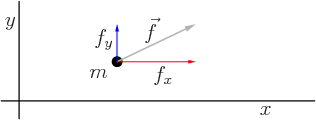
\includegraphics{function_as_vector1}
\caption{Vector $\vec{f}$ as sum of component vectors $\vec{f_x}$ and $\vec{f_y}$.}
\end{figure}

This vector $\vec{f}$ can be expressed as sum of its projection onto axes x and y (respectively $\vec{f_x}$ and $\vec{f_y}$. These two component vectors can be represented in a different way, called \textit{spike diagram}:

\begin{figure}[ht]
\centering
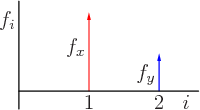
\includegraphics{function_as_vector2}
\caption{Component vectors presented in spike diagram.}
\end{figure}

We can notice, that with each new dimension added to the space, in which the vector is considered, we just add one new spike in the spike diagram representation. Below is given an example of vector in 3D space and another one in space with much larger number of dimensions:

\begin{figure}[ht]
\centering
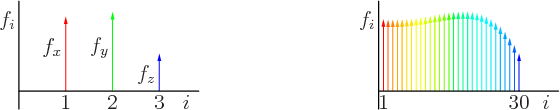
\includegraphics[scale=0.75]{function_as_vector3}
\caption{Left: vector in 3D space. Right: vector in many-dimensional space.}
\end{figure}

If we follow this reasoning, we can consider a vector with an infinite number of dimensions as a spike diagram with infinitely many spikes. This can be in turn represented on a continuous coordinate (e.g. \textit{x}):

\begin{figure}[ht]
\centering
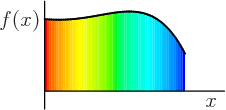
\includegraphics{function_as_vector4}
\caption{Vector with infinite number of dimensions.}
\end{figure}

We can see, that top boundary of the area made of spikes is some function $f(x)$. We have received a direct transition between the concept of a vector and a function - a function can be seen as a vector with infinitely many dimensions. It is worth noticing, that each function can be understood as a vector, but not the other way.

In this work, even when discussing functions, we will represent them in the form of vectors. We will give examples in 2D and 3D spaces, whose aim is to develop intuition about the discussed concept and which can be expanded to a larger number of dimensions.

\subsection{Complex and Hermitian conjugates}

\begin{example}
For a given vector $z$ in a complex space we can create a \textbf{complex conjugate} of such a vector (noted as $\overline{z}$ or $z^*$) in the following way:

\begin{figure}[ht]
\centering

\includegraphics[scale=0.5]{complex_conjugate}
\caption{A vector \textit{z} and its complex conjugate.}
\end{figure}

We can write this in a matrix form as:

\[ z_1 = \begin{pmatrix} 10 \\ i \end{pmatrix}, \ z_{1}^* = \begin{pmatrix} 10 \\ -i \end{pmatrix}  \]

\[ z_2 = \begin{pmatrix} e^{i} \\ i \end{pmatrix}, \ z_{2}^* = \begin{pmatrix} e^{-i} \\ -i \end{pmatrix}  \]
\end{example}

\begin{example}
In a similar way, for a vector \textit{z} we can introduce its \textbf{Hermitian conjugate} as

\[ z = \begin{pmatrix} e^{i} \\ i \end{pmatrix}, \ z^{\dagger} = \begin{pmatrix} e^{-i} & -i \end{pmatrix}, \]

which is equivalent to apply a complex conjugate and a transposition
\[  z^\dagger = (z^*)^T. \]
\end{example}

\begin{example}
The same procedure can be applied to matrices:
\[ M = \begin{pmatrix} 1 & i \\ e^i & 2 \end{pmatrix}, \ M^* = \begin{pmatrix} 1 & -i \\ e^{-i} & 2 \end{pmatrix} \]
\[ M^\dagger = \begin{pmatrix} 1 & e^{-i} \\ -i & 2 \end{pmatrix} \]
\end{example}

\subsection{A vector space and a function space}

\begin{definition}
Let $(\mathbb{F}, +, \cdot)$ be a field (reader can think of this as real or complex numbers). Let X be any nonempty set. Elements of $\mathbb{F}$ and X will be called respectively scalars and vectors. Let's introduce two two-argument operations:
\begin{enumerate}
    \item addition of vectors: $X \times X \rightarrow X$ noted as $x + y$ for $x, y \in X$,
    \item multiplication by scalar: $\mathbb{F} \times X \rightarrow X$, noted as $a \cdot x$ for $a \in \mathbb{F}$ and $x \in X$.
\end{enumerate}
Set X with operations $+$ and $\cdot$ is called a \textbf{vector space} (or \textbf{linear space}) if for any $a,b \in \mathbb{F}$ and $x,y,z \in X$ it fulfills following conditions:
\begin{legal}
    \item $x + y = y + x$ (commutative property),
    \item $x + (y + z) = (x + y) + z$ (associative property of addition),
    \item there exists element $0 \in X$, such that for any $x \in X$, $x + 0 = x$,
    \item for any $x \in X$ exists an opposite element $-x \in X$, such that $x + (-x) = 0$,
    \item $a(x + y) = ax + ay$ (left-distributive property),
    \item $(a + b)x = ax + bx$ (right-distributive property),
    \item $a(bx) = (ab)x$ (associative property of multiplication),
    \item there exists a scalar $1 \in \mathbb{F}$, such that for any $x \in X$, $1 \cdot x = x$.
\end{legal}
Such a vector space is going to be noted as $\langle X, +, \cdot \rangle$.
\end{definition}

\begin{remark}
When we consider fields of real or complex numbers it will be noted respectively $\mathbb{F} = \mathbb{R}$ and $\mathbb{F} = \mathbb{C}$.
\end{remark}

\begin{definition}
Let V be a vector space over the field $\mathbb{F}$ and let X be some set. A set of functions $\{f: X \rightarrow V\}$ with two operations:
\begin{legal}
    \item addition of functions: \\ 
    For any two functions $f, g: X \rightarrow V$, for any $x \in X$, there is a function $h: X \rightarrow V$, such that $h(x) = f(x) + g(x)$,
    \item multiplication of a function by a scalar: \\
    For any function $f: X \rightarrow V$ and scalar $a \in \mathbb{F}$ there is a function $h: X \rightarrow V$ such that $h(x) = a \cdot f(x)$,
\end{legal}
is called a \textbf{function space}.
\end{definition}

\begin{remark}
Function space can be understood as a vector space, whose points are functions.
\end{remark}

It is important to notice, that a term \textit{vector} from the definition of a \textit{vector space} has to be understood differently from the common concept of a vector (arrow with given length, attachment point and direction). In our understanding \textit{vector} is any object, that meets the requirements of vector space, so it can be e.g. a square matrix $n \times n$, a function or a point.

Another noteworthy issue is the \textit{geometric interpretation of vector}. It is very convenient way to visualize a vector as an arrow in e.g. an euclidean 3D space, but this method does not hold for all vector spaces. First of all, it is hard to visualize a vector in more than three dimensions. Secondly, the \textit{direction} property of a vector diminishes, when we are considering unordered fields. Such a field is for example a field of complex numbers $\mathbb{C}$. Let's say, that we can introduce order in the $\mathbb{C}$ field. We have to notice, that $\mathbb{R}$ is a subset of $\mathbb{C}$, so the order imposed on $\mathbb{C}$ should be also correct for $\mathbb{R}$. Unfortunately, this is not possible. Such an order should harmonize with operations of addition and multiplication in these fields. But it is obvious, that for $\mathbb{R}$ we have, that $\forall x \in \mathbb{R}\  x^2 \geq 0$, which does not hold for $\mathbb{C}$ (e.g. $i^2 < 0$). As a result, when we cannot compare two numbers in $\mathbb{C}$ it is incorrect to talk about vector's direction.

\begin{definition}
For a given vector space X over the field $\mathbb{F}$ we define \textbf{basis} as a subset $B \subseteq X$ such that:
\begin{legal}
    \item B is linearly independent,
    \item any $x \in X$ can be written as a linear combination of elements $b \in B$.
\end{legal}
\end{definition}

\subsection{Operators and functionals}

\begin{definition}
Let X and Y be two vector spaces over the field $\mathbb{F}$. A projection $\hat{T}: X \rightarrow Y$ is called a \textbf{linear operator} if for any $x,y \in X$ and $a \in \mathbb{F}$
\begin{legal}
    \item $\hat{T}(x + y) = \hat{T}(x) + \hat{T}(y)$ (additivity),
    \item $\hat{T}(ax) = a\hat{T}(x)$ (homogeneity).
\end{legal}
If $Y = \mathbb{F}$ and T takes the form $\hat{T}: X \rightarrow \mathbb{F}$ it is called a \textbf{functional}.
\end{definition}

\begin{remark}
A functional can be understood as a special case of operator, which instead of returning vector returns scalar (or one-dimensional vector).
\end{remark}

\begin{example}
A simple example of an operator is a \textit{differential operator}, which takes as an input one function and returns the other one:
\[ \frac{d}{dx} f(x) = g(x). \]
\end{example}

\begin{example}
An \textit{integral} is a great example of a functional (it takes some function \textit{f} as an input and returns a number).
\end{example}

From the above definition we know, that an operator takes a vector as its input and outputs some other vector. This operation can be expressed in the form of a matrix.

\begin{example}
Let's say we have an operator $\hat{T}$ and vectors $a = \begin{pmatrix} 1 \\ 2 \end{pmatrix}$ and $b = \begin{pmatrix} 5 \\ 11 \end{pmatrix}$. We have, that
\[ \hat{T}(a) = b, \]
which can be expressed in the matrix form
\[ \hat{T}\begin{pmatrix} 1 \\ 2 \end{pmatrix}  = \begin{pmatrix} 5 \\ 11 \end{pmatrix}.\]
We can see, that $\hat{T}$ can be expressed as a matrix $\begin{pmatrix} 1 & 2 \\ 3 & 4 \end{pmatrix}$:
\[ \begin{pmatrix} 1 & 2 \\ 3 & 4 \end{pmatrix} \begin{pmatrix} 1 \\ 2 \end{pmatrix} = \begin{pmatrix} 5 \\ 11 \end{pmatrix}. \]
\end{example}

Action of an operator can be understood in two ways:
\begin{legal}
    \item it rotates the vector around the basis:
    \begin{figure}[ht]
        \centering
        \begin{minipage}{.5\textwidth}
          \centering
          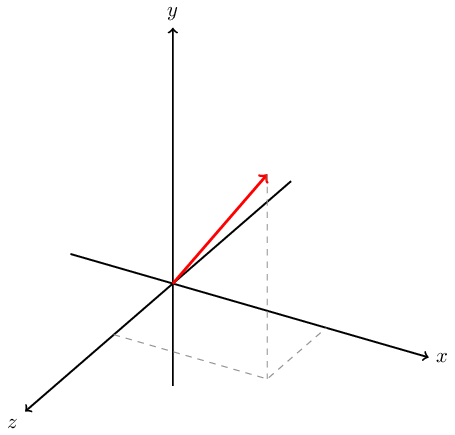
\includegraphics[width=.6\linewidth]{original_vector}
          \captionof{figure}{Original vector.}
        \end{minipage}%
        \begin{minipage}{.5\textwidth}
          \centering
          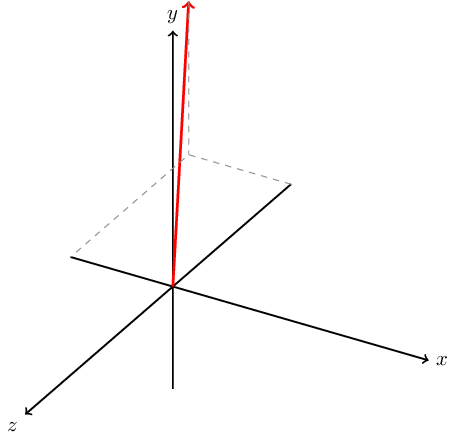
\includegraphics[width=.6\linewidth]{rotated_vector}
          \captionof{figure}{Rotated vector.}
        \end{minipage}
    \end{figure}
    \item it rotates the basis and leaves the vector unchanged:
    \begin{figure}[ht]
        \centering
        \begin{minipage}{.5\textwidth}
          \centering
          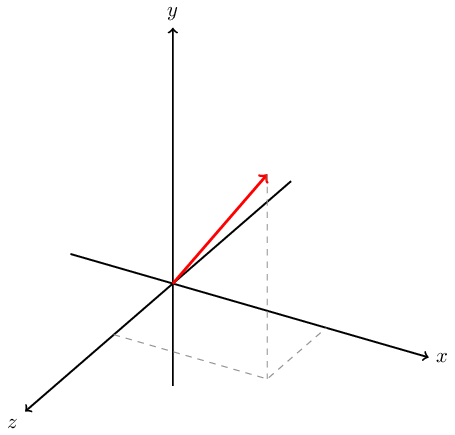
\includegraphics[width=.6\linewidth]{original_vector}
          \captionof{figure}{Original vector.}
        \end{minipage}%
        \begin{minipage}{.5\textwidth}
          \centering
          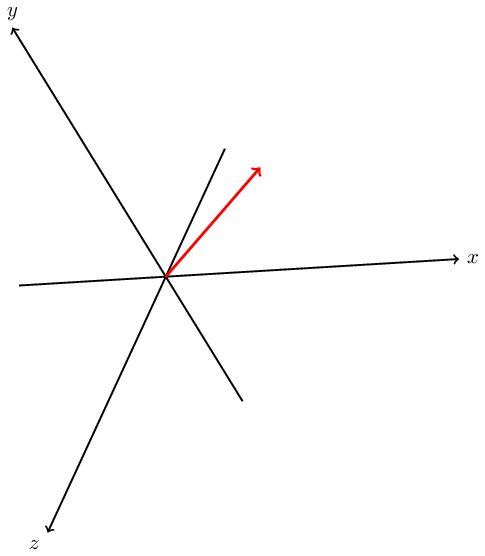
\includegraphics[width=.6\linewidth]{rotated_basis}
          \captionof{figure}{Rotated basis.}
        \end{minipage}
    \end{figure}
\end{legal}

\subsection{From a vector space to a Hilbert space}

In this subsection we will gradually expand definition of a vector space with new features and finally we will introduce an inner product space, which will be essential in next chapters (however the concept of topological space will not be discussed in this work). Relationships between different kinds of spaces are given in the picture below.

\begin{figure}[ht]
\centering
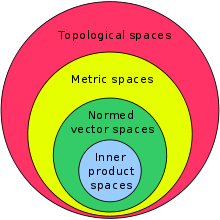
\includegraphics{spaces}
\caption{Relationships between spaces.}
\end{figure}

\begin{definition} \label{metric_space}
Let X be a nonempty set and d be a functional, $d: X \times X \rightarrow \mathbb{F}_{0}$ (where $\mathbb{F}_0$ are non-negative elements of field $\mathbb{F}$), called a \textbf{metric} (or a distance), if it meets the following requirements (for any $x,y,z \in X$):
\begin{legal}
    \item $d(x, y) = 0$ if and only if $x = y$,
    \item $d(x, y) = d(y, x)$,
    \item $d(x, y) \leq d(x, z) + d(z, y)$.
\end{legal}

A set X with a metric d is called a \textbf{metric space} and is noted as $\langle X, d \rangle $.
\end{definition}

\begin{definition}
For a set X let us consider sequence $(x_i)$, where $x_i \in X$. Such sequence is called \textbf{Cauchy sequence}, if
\[ \forall_{\epsilon > 0} \ \exists_{N \in \mathbb{N}} \ \forall_{m,n > N} \ d(x_m, x_n) < \epsilon. \]
\end{definition}

\begin{definition}
A metric space $\langle X, d \rangle$ is called \textbf{complete}, if every Cauchy sequence converges to an element of X.
\end{definition}

\begin{definition}
Let X be a vector space over the field $\mathbb{F}$. We define a functional performing $ x \rightarrow \norm{x}$, where $ x \in X$ and $\norm{x}$ is a non-negative element of X. It is called a \textbf{norm}, if for any $x,y \in X$ and $a \in \mathbb{F}$ it has the following properties:
\begin{legal}
	\item $\norm{x}$ = 0 implies $x = 0$,
	\item $ \norm{x + y} \leq \norm{x} + \norm{y}$ (triangle inequality),
	\item $\norm{ax} = |a| \cdot \norm{x}$ (norm is homogeneous).
\end{legal}
\end{definition}

\begin{definition}
A pair $\langle X, \norm{\cdot} \rangle$, where X is a vector space and $\norm{}$ is a norm in it, is called a \textbf{normed space}.
\end{definition}

\begin{definition}
Let X be a vector space over the field $\mathbb{F}$ with a functional $f: X \times X \rightarrow \mathbb{F}$ noted as $\langle x | y \rangle$ for $x,y \in X$. If f meets the following requirements:
\begin{legal}
    \item $\langle x + y | z\rangle = \langle x | z \rangle + \langle y | z \rangle$,
    \item $\langle ax | y \rangle = a\langle x | y \rangle$,
    \item $\langle y | x\rangle = \langle x | y \rangle^\dagger$,
    \item $\langle x | x \rangle > 0$ for $x \neq 0$,
\end{legal}
it is called an \textbf{inner product} (or a \textbf{dot product}) and the pair $\langle X, \langle\cdot | \cdot\rangle \rangle$ is called an \textbf{inner product space}. When $\langle X, \langle\cdot | \cdot\rangle \rangle$ is over the field $\mathbb{C}$, the name \textbf{unitary space} is used, when referring to it.
\end{definition}

\begin{remark}
An inner product can be understood in terms of vectors projection. Below is given an example in Euclidean space:


\begin{figure}[ht]
\centering
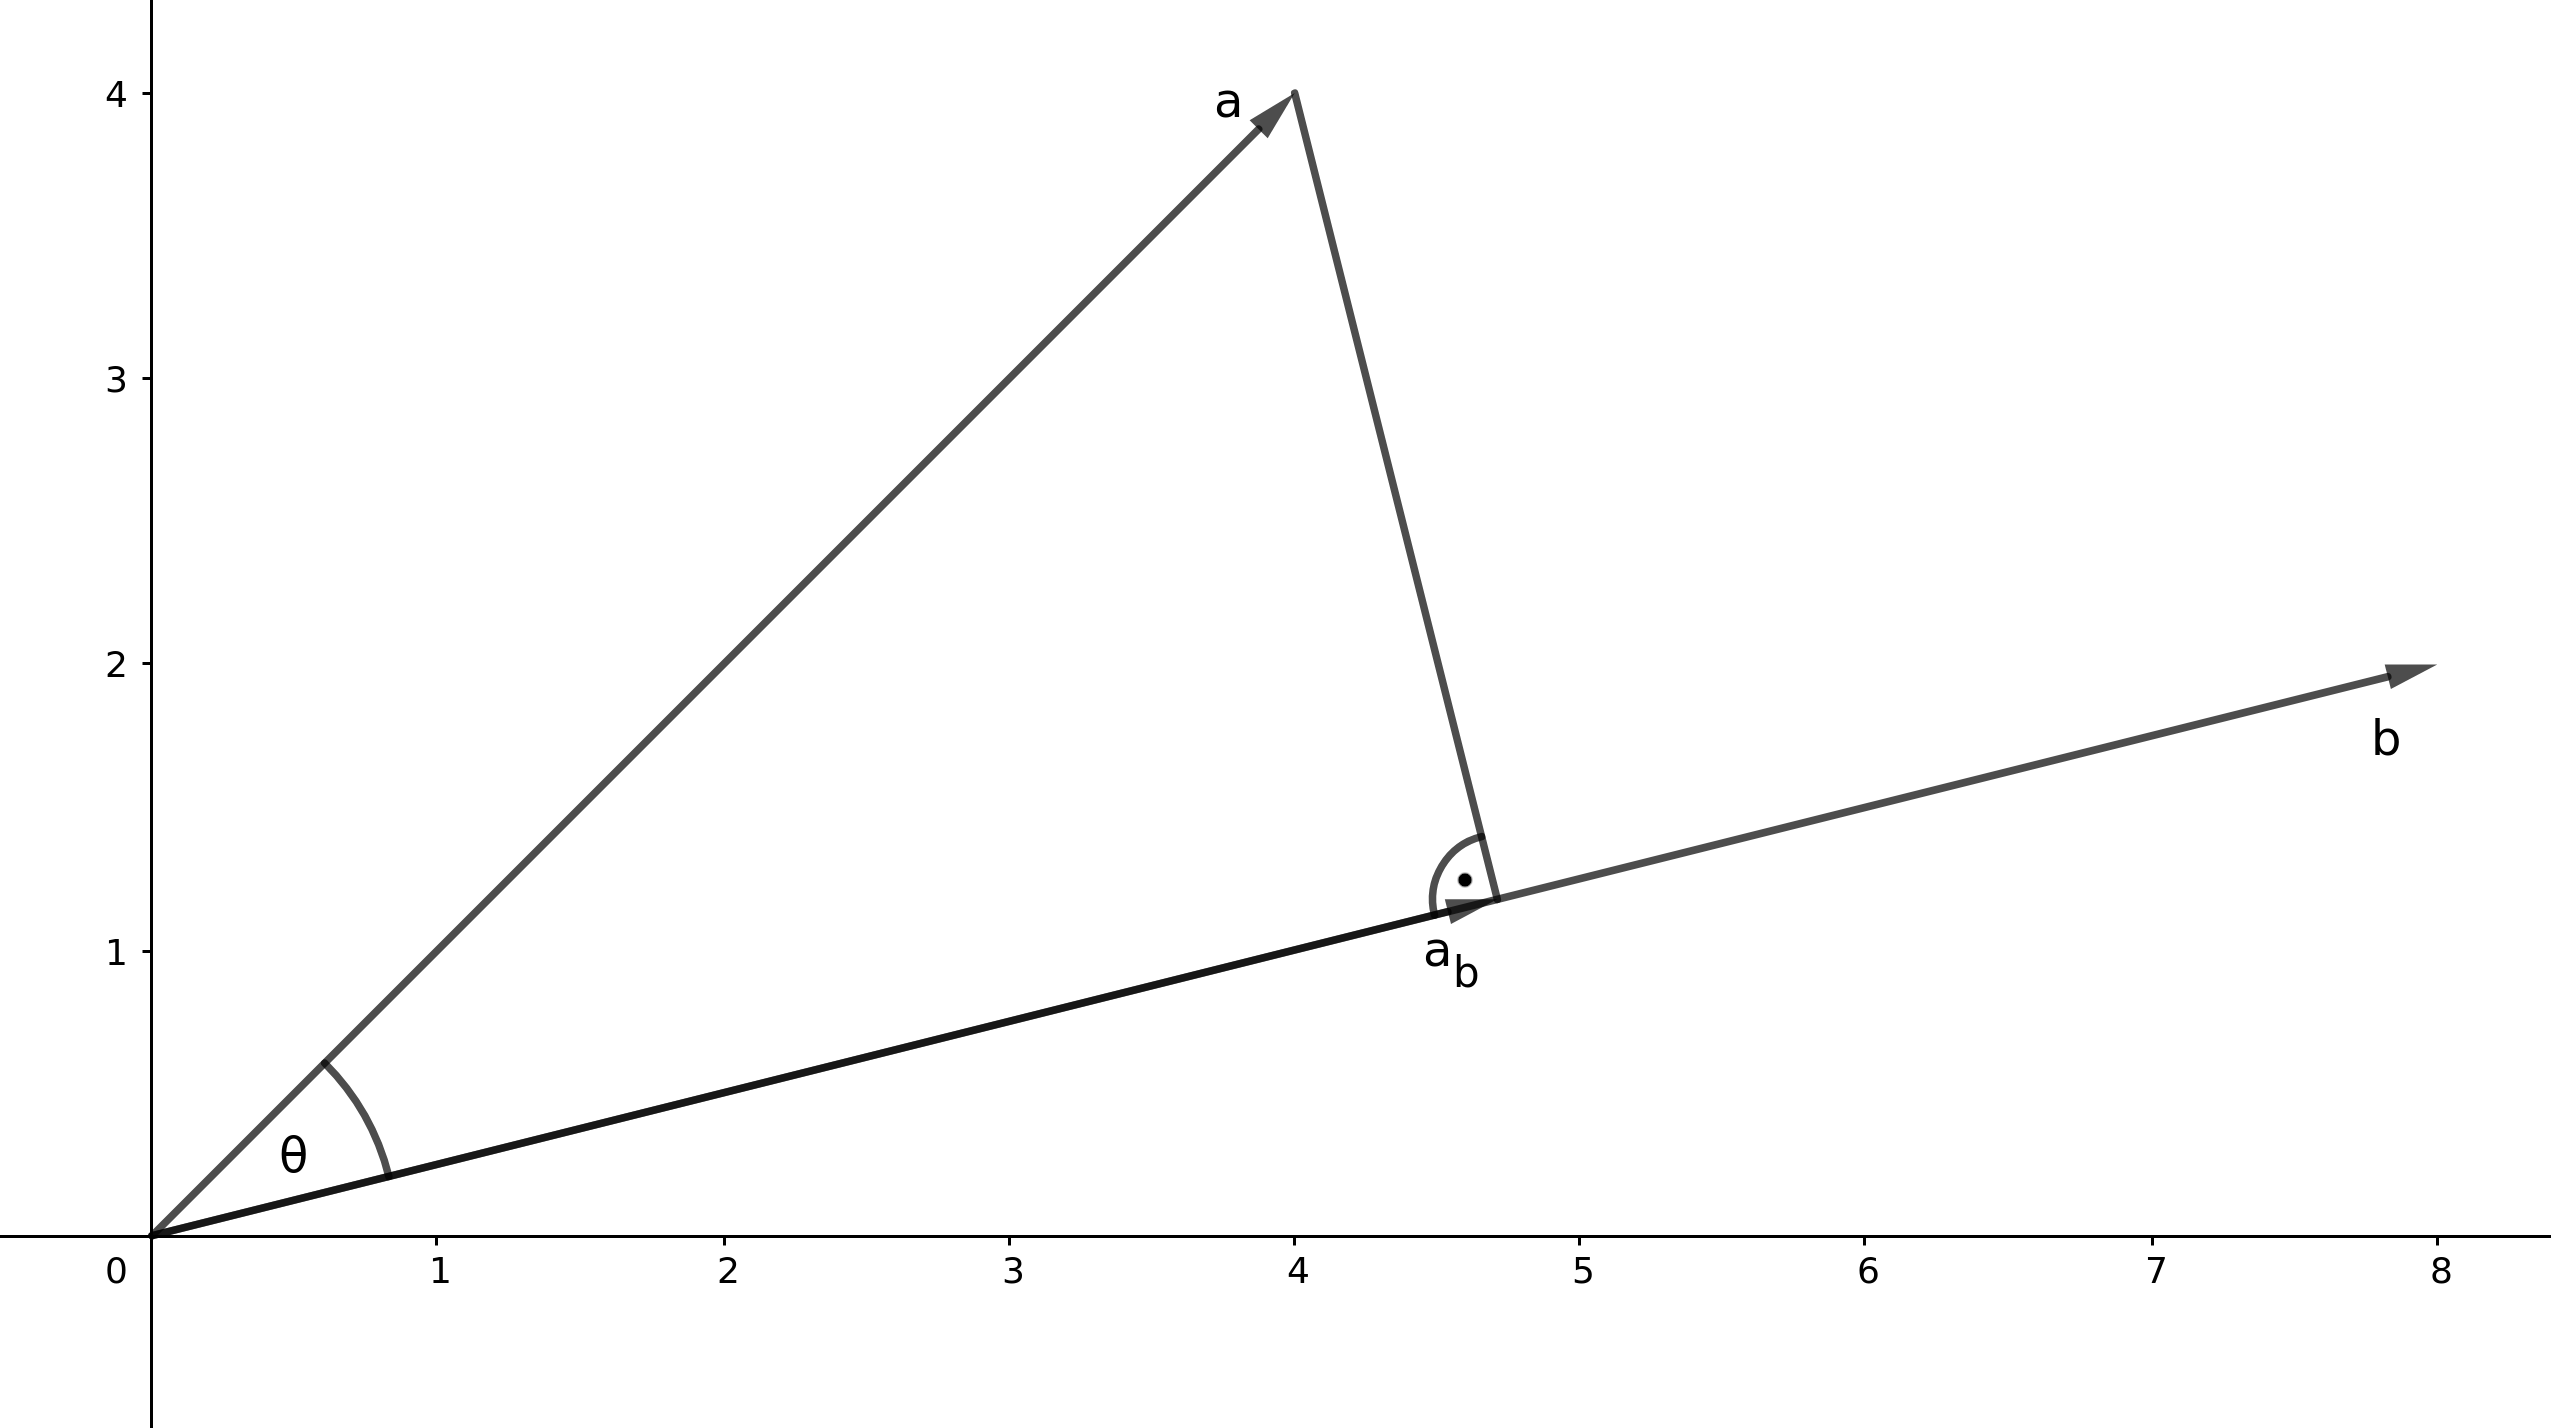
\includegraphics[scale=0.15]{vectors_projection}
\caption{A geometrical interpretation of inner product.}
\end{figure}

In such a case, we define an inner product as
\[ \boxed{\langle a | b\rangle = \norm{a} \norm{b} cos(\theta)}.\]

We can see, that 
\[\norm{a_b} = cos(\theta) \norm{a}, \] 
so 
\[ \boxed{\langle a | b\rangle = \norm{a} \norm{b} cos(\theta) = \norm{a_b} \norm{b}}. \]

We have shown, that an inner product can be understood as a multiplication of the norm of projection of the vector a onto b and the norm of the vector b.

Let's consider an inner product $\langle a | a \rangle$. As shown above, it can be understood as a projection of the vector a onto itself. Due to this, a result of such an operation equals

\[ \langle a | a \rangle = \norm{a_a} \norm{a} = \norm{a} \norm{a} = \norm{a}^2.  \]

This implies, that a norm in an inner product space is defined as

\[ \boxed{\norm{a} = \sqrt{\langle a | a \rangle}}.  \]
\end{remark}

\begin{definition}
If an inner product space X is complete due to the metric induced by the inner product (through the norm) it is called a \textbf{Hilbert space}.
\end{definition}

\begin{remark}
We have previously shown the dependence between a norm and an inner product
\[ \norm{x} = \sqrt{\langle x | x \rangle}. \]
It is important to notice, that a \textbf{norm is a real-valued functional}. When we say, that a metric is induced by a norm, it can be written as
\[  d(x, y) = \norm{x - y} = \sqrt{\langle x-y | x-y \rangle}. \]
\end{remark}

\begin{remark}
An inner product in a Hilbert space is defined as follows
\[ \langle x | y \rangle = x^\dagger y.\]
An inner product defined in such a way always returns real-valued numbers (even when a Hilbert space is over the field $\mathbb{C}$).
\end{remark}

\subsection{Normalization, ortogonality and orthonormality of vectors}

\begin{definition}
Let $\langle X, \langle \cdot | \cdot \rangle \rangle$ be an inner product space over the field $\mathbb{F}$ and $x,y \in X$. We say, that x and y are \textbf{orthogonal}, if $\langle x | y\rangle = 0$. We denote this as $x \perp y$.
\end{definition}

\begin{definition}
Let $\langle X , \norm{\cdot} \rangle$ be a normed space. An \textbf{unitary vector} v (also called a \textbf{versor}) is a vector, for which $\norm{v} = 1$.
\end{definition}

\begin{remark}
For any vector v (from a normed space) we can define a procedure called a \textbf{normalization}, thanks to which it can be changed to unitary vector $v^0$:
\[ v^0 = \frac{v}{\norm{v}} = \frac{v}{\sqrt{\langle v | v \rangle}} \]
\end{remark}

\begin{remark}
When all of the vectors $\{v_i\}_{i=1}^n$ spanning a vector space (base vectors) have a length equal to 1 ($\norm{v_i} = 1$), we call such a base a \textbf{normalized base}.
\end{remark}

\begin{definition}
Let $\langle X, \norm{\cdot} \rangle$ be a normed space and $x,y \in X$. We say, that x and y are \textbf{orthonormal}, when
\[ \langle x | y \rangle = 
\begin{cases} 
    1, & if \  x = y \\
    0, & if \  x \neq y
\end{cases}
\]
An orthonormality is just an extension of an ortogonality (two vectors are ortogonal and have a length equal to 1).
\end{definition}

\begin{remark}
A normalized base is a base made of orthonormal vectors.
\end{remark}

\subsection{Unitary and Hermitian operators}

\begin{definition}
We say, that for vector spaces X and Y, an operator $\hat{T}: X \rightarrow Y$ is \textbf{unitary}, if the following occurs
\[ \hat{T}\hat{T}^\dagger = I, \]
where I is the identity operator. I may be understood as the identity matrix
\[ I = \begin{pmatrix} 1 & 0 \\ 0 & 1 \end{pmatrix}.  \]
\end{definition}

\begin{remark} \label{unitary_operators_no_length_change}
This remark is extremely important because of the correct understanding of the further part of the work. \textbf{Unitary operators applied to vectors do not change their length} (vectors are only \textbf{rotated}).
\end{remark}

\begin{definition}
For vector spaces X and Y, an operator $\hat{T}: X \rightarrow Y$ is called \textbf{Hermitian} (or \textbf{self-adjoint}), if
\[ \hat{T} = \hat{T}^\dagger. \]
\end{definition}

\subsection{Eigenvector, eigenfunction and eigenvalue of an operator}

\begin{definition}
For any operator $\hat{T}$ we can write the following linear equation:
\[ \hat{T} x = \lambda x, \]
where x is called an \textbf{eigenvector} and $\lambda$ is called an \textbf{eigenvalue}.
When we are considering a function space instead of a vector space, the above equation takes the following form:
\[  \hat{T} f = \lambda f, \]
and f is called an \textbf{eigenfunction}.
\end{definition}

\newpage
\section{Basics of quantum mechanics}

We will begin this section by introducing some notation. Later, we will present six postulates of quantum mechanics, after which we will provide an example illustrating a counter-intuitive behavior of quantum entities. Finally, we will explain the use of a tensor product in the description of more complicated physical systems and give a short introduction to the concept of entaglement.

\subsection{Bra-ket notation, Kronecker and Dirac deltas}

\begin{definition}
Every vector $\vec{x}$ can be written in the form
\[ | x \rangle \equiv \begin{pmatrix} x_1 \\ x_2 \\ \cdot \\ \cdot \\ \cdot \\ x_n \end{pmatrix}, \]
which is called the \textbf{ket} notation.
\end{definition}

\begin{definition}
Any Hermitian conjugate of a vector $\vec{x}$ can be written as
\[ \langle x | \equiv \begin{pmatrix} x_1^* & x_2^* & \cdot \cdot \cdot & x_n^* \end{pmatrix}, \]
which is called the \textbf{bra} notation.
\end{definition}

\begin{remark}
We have previously stated, that an inner product in Hilbert spaces is defined as
\[ \langle x | y \rangle = x^\dagger y.\]
Note, that it can be also written in the bra-ket notation in the following way
\[ \langle x | y \rangle = \begin{pmatrix} x_1^* & x_2^* & \cdot \cdot \cdot & x_n^* \end{pmatrix} \begin{pmatrix} y_1 \\ y_2 \\ \cdot \\ \cdot \\ \cdot \\ y_n \end{pmatrix} = x^\dagger y,\]
which is consistent with the notation, which we used earlier to denote the inner product.
\end{remark}


\begin{definition}
We define a symbol called \textbf{Kronecker delta} (noted as $\delta_{ij}$) in the following way
\[ \delta_{ij} = \begin{cases}
    0,\ if\ i \neq j \\
    1,\ if\ i = j
\end{cases} \]
\end{definition}

\begin{definition}
We define a \textbf{Dirac delta function} as
\[ \delta(x) = \begin{cases}
    +\infty, \ if \ x = 0 \\
    0, \ \ \ \ \ if \ x \neq 0
\end{cases}\]
with an additional constraint
\[ \int_{-\infty}^{+\infty} \delta(x)dx = 1. \]
\end{definition}

\subsection{Postulates of quantum mechanics}

When describing a mathematical model simulating quantum physics we use Hilbert spaces over the field $\mathbb{C}$ (that is why we needed to introduce all the definitions in the previous section). At the beginning it is important to notice, that although we are operating in a space with complex numbers, a result of an inner product is always real-valued. This property of the Hilbert space is indispensable, while creating model with a practical application, because results of measurements of physical systems are always real-valued.

Below we introduce six postulates, which for quantum physics are what axioms for mathematics are.

\begin{postulate}
State of a physical system can be represented by a \textbf{state function} $|\psi \rangle$, also called a \textbf{wave function}. It has to be continuous and differentiable. It contains all possible information about the system.
\end{postulate}

\begin{definition}
Every measurable physical property T is called an \textbf{observable}. It can be understood as e.g. an energy, a momentum, a mass or an angular momentum.
\end{definition}

\begin{postulate}
Every observable T is described by an operator $\hat{T}$. 
\end{postulate}

\begin{postulate}
Every measurement of an observable T can only give one of the eigenvalues $\lambda$ of the operator $\hat{T}$ (associated with this physical property), that is
\[ \hat{T} |\psi\rangle = \lambda |\psi \rangle,  \]
where $|\psi \rangle$ is an eigenfunction of the operator $\hat{T}$.
\end{postulate}

\begin{postulate}
The probability, that measurement will return an eigenvalue $\lambda$ is equal to $| \langle \psi_\lambda | \psi \rangle |^2$, where $\langle \psi_\lambda | \psi \rangle = c_\lambda$ is called a \textbf{probability amplitude}.
\end{postulate}

\begin{remark}
We say, that a system before measurement is in a \textbf{superposition} of all eigenfunctions (that is, it is a sum of all its eignefunctions). It can be written, as
\[ | \psi \rangle = \sum_n \langle \psi_n | \psi \rangle |\psi_n \rangle = \sum_n c_n | \psi_n \rangle. \]
Usually eigenstates are normalized, so
\[ \langle \psi_i | \psi_j \rangle = \delta_{ij}. \]
When we are considering a case with a continuous set of egienstates, we have to use the Dirac's $\delta$-function
\[ \langle \psi_i | \psi_j \rangle = \delta(\psi_i - \psi_j). \]
If eigenfunctions are normalized, we can write (for a discrete case of measurements' results)
\[ \sum_n c_n = 1. \]
While considering a probability of finding a result of a measurement of an observable T in an interval [T, T + dT] equal to P(T)dT, we obtain
\[ \int_{-\infty}^{+\infty} P(T)dT = 1. \]
A set of normalized eigenfunctions is said to create a basis of the wave function $| \psi \rangle$.
\end{remark}

\begin{definition}
We designate the \textbf{expected value} of an observable T as $\langle T \rangle$. If measurements of T return discrete values $T_i$ (with the same probability), it can be written as
\[  \langle \hat{T} \rangle = \frac{1}{N} \sum_{i = 1}^N T_i,\]
where N is a number of all possible outcomes. It can be also expressed in terms of probability $P(T_i)$
\[ \langle \hat{T} \rangle = \sum_{i=1}^N T_i P(T_i). \]
If results of a measurement of T create a continuous set, we denote this as
\[ \langle \hat{T} \rangle = \int_{-\infty}^{+\infty} T P(T) dT, \]
where P(T) is a probability density function. Concluding from the above we can say, that P(T)dT is a probability of obtaining T in the interval [T, T + dT]. 
\end{definition}

\begin{remark}
We write the expected value of an observable T (for a discrete case) as
\[ \langle \hat{T} \rangle = \langle \psi | \hat{T} | \psi \rangle = \sum_{i} \sum_{j} c_i^*c_j \langle \psi_i | \hat{T}|\psi_j\rangle = \sum_{i} \sum_{j} c_i^* c_j \langle \psi_i | \psi_j \rangle \lambda_j = \sum_{i} |c_i|^2 \lambda_i \]
Now, we are going to use the equation for calculating the eigenfunction of $\hat{T}$
\[ \hat{T} |\psi_n \rangle = \lambda_n |\psi_n \rangle, \]
where $|\psi_n \rangle$ is the n-th eigenfunction of the operator $\hat{T}$. We obtain
\[ \sum_n \psi_n^* \hat{T} \psi_n = \sum_n \psi_n^* \lambda_n \psi_n = \sum_n \lambda_n \psi_n^* \psi_n = 
\sum_n \lambda_n | \langle \psi_n | \psi_n\rangle |^2 = \sum_n \lambda_n | c_n |^2 .\]
Summarizing we can write, that in a discrete case, the expected value of an observable T equals to
\[ \boxed{\langle \hat{T} \rangle = \sum_n \lambda_n | c_n |^2} \]
This reasoning can be extended to the case with a continuous set of measurements' results
\[ \langle \hat{T} \rangle = \int_{-\infty}^{+\infty} T P(T) dT. \]
\end{remark}

\begin{postulate}
A measurement of an observable of a physical system (associated with an operator $\hat{T}$), returning a value $\lambda$, leaves this system in a state $|\psi_\lambda \rangle$, where
\[ \hat{T} |\psi_\lambda\rangle = \lambda \ |\psi_\lambda\rangle \]
($|\psi_\lambda \rangle$ is the eigenfunction of the operator $\hat{T}$, corresponding to the eigenvalue $\lambda$). This is often referred as to a \textbf{collapse} of the system.
\end{postulate}

\begin{postulate}
A wave function of a physical system depends on a time according to the \textbf{time dependent Schr\"odinger equation}
\[ i\hbar \frac{\partial}{\partial t}\psi(\vec{r}, t) = \hat{H}\psi(\vec{r}, t), \]
where $\psi(r, t)$ is a wave function dependent from a position $\vec{r}$ and a time t and $\hat{H}$ is an energy operator called \textbf{hamiltonian}.
\end{postulate}

\newpage
\subsection{Illustrative example - Stern-Gerlach experiment}

This experiment measures the magnetic moment caused by the spin of an elementary particle, called \textbf{spin magnetic moment}. To better understand this property, reader can visualize it as a spinning electron (although this analogy is not completely correct). Particles can only have quantized (discrete) values of a spin. Electrons are said to have a spin $+\frac{1}{2}$ or $-\frac{1}{2}$, which is denoted as $| + \rangle$ and $|-\rangle$ respectively. Because of this, a state of an electron's spin before a measurement can be written as
\[ | \psi \rangle = \frac{1}{\sqrt{2}}(|+\rangle + |-\rangle ), \]
which is equal to
\[ |\psi \rangle = \begin{pmatrix} \frac{1}{\sqrt{2}} \\  \frac{1}{\sqrt{2}} \end{pmatrix}. \]
Values next to the possible outcomes $|+\rangle$ and $|-\rangle$ are equal to $\frac{1}{\sqrt{2}}$, because a measurement returns each of these options with probability $|\frac{1}{\sqrt{2}}|^2$, so an electron have a 50\% probability of having a spin $|+\rangle$ and 50\% of having a spin $|-\rangle$.
\begin{remark}
As mentioned in the previous subsection, an electron before a measurement is in a \textbf{superposition} of states having spins $|+\rangle$ and $|-\rangle$. During the experiment it collapses to only one of the possible outcomes.
\end{remark}

When an electron moves in a presence of a magnetic field, because of its spin it will deflect in some direction. We can introduce a device, which uses this phenomenon to measure an electron's spin along a given axis. We can create such a field, that an electron in its presence will deflect upwards, if it has a $|+\rangle$ spin along z axis, and downwards, if it has a $|-\rangle$ spin. It will be presented as a black-box

\begin{figure}[ht]
\centering
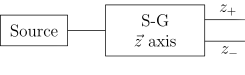
\includegraphics{stern_gerlach_device}
\caption{A Stern-Gerlach device recognizing the electron's spin along z axis.}
\end{figure}

A notation $z_+$ means, that an electron has the spin $|+\rangle$ along z axis and $z_-$, that it has the $|-\rangle$ spin along z axis. For the purpose of this thought experiment Let's assume, that an electron is in a state $|\psi \rangle$ mentioned above ($| \psi \rangle = \frac{1}{\sqrt{2}}(|+\rangle + |-\rangle )$). In such a case, an electron has 50\% chances of deflecting upwards, and 50\% of deflecting downwards. \newline

When an electron's spin collapses after the experiment in one of the possible outcomes, next experiments (measuring the same property) will return the same result

\begin{figure}[ht]
\centering

\includegraphics[scale=0.7]{stern_gerlach_consecutive_z_axis.png}
\caption{Two consecutive measurements of the electron's spin along z axis.}
\end{figure}

In the above experiment, after the first measurement the electron's spin collapsed to the state $|+\rangle$ (along z axis) and because of this, the second measurement of this property returned the same result.\newline

Another important phenomenon, is that a measurement of a spin along one axis does not affect the result of a measurement along other axes.

\begin{figure}[ht]
\centering

\includegraphics[scale=0.7]{stern_gerlach_different_axes}
\caption{Two consecutive measurements of the electron's spin along different axes.}
\end{figure}

In the experiment above the electron had the $|+\rangle$ spin along z axis, but it did not influence the measurement of the spin along x axis (it still had 50\% chances of having the $|+\rangle$ spin and 50\% of having the $|-\rangle$ spin).\newline

Finally, a measurement of a spin along one axis erases all information gathered about this property along other axes. It is presented at the picture below

\begin{figure}[ht]
\centering

\includegraphics[scale=0.7]{stern_gerlach_deletion_of_information}
\caption{The deletion of information about the electron's spin along z axis.}
\end{figure}

In the first measurement the electron had the $|+\rangle$ spin along z axis. Later, the spin along x axis was measured, which made, that the electron again had 50\% chances of having the $|+\rangle$ spin and 50\% of having the $|-\rangle$ spin along z axis.

\subsection{Description of compound systems - tensor product and entanglement}

Let's say, we want do describe the behavior of a physical system made up of many simpler systems e.g. an interaction between two elementary particles. We will call all of the possible states, in which the first particle can be, as a set \textit{A}, and all possible states of the second particle as a set \textit{B}. If states of these two quantum entities are independent from each other, the whole system (two particles) can be described as a \textbf{tensor product} of the set A with the set B. On the other hand, if states of these two particles are not independent, we say that they are \textbf{entangled}.

\begin{definition}
The \textbf{tensor product} (or the \textbf{Kronecker's product}) of two matrices A and B, where $A \in M_{m\times n}$ and $B \in M_{k \times l}$ is a block matrix $C \in M_{mk \times nl}$ of the form
\[ C = A \otimes B  = \begin{pmatrix} a_{11} & a_{12} & \cdots & a_{1n} \\
a_{21} & a_{22} & \cdots & a_{2n} \\ \vdots & \vdots & \ddots & \vdots \\ a_{m1} & a_{m2} & \cdots & a_{mn}\end{pmatrix} \otimes \begin{pmatrix} b_{11} & b_{12} & \cdots & b_{1l} \\
b_{21} & b_{22} & \cdots & b_{2l} \\ \vdots & \vdots & \ddots & \vdots \\ b_{k1} & b_{k2} & \cdots & b_{kl}\end{pmatrix} = \]


\[\begin{pmatrix}
a_{11}b_{11} & a_{11}b_{12} & \cdots & a_{12}b_{11} & a_{12}b_{12} & \cdots \\
a_{11}b_{21} & a_{11}b_{22} &  & a_{12}b_{21} & a_{12}b_{22} &  \\
\vdots \\
a_{11}b_{k1} & a_{11}b_{k2} & \cdots & a_{12}b_{k1} & a_{12}b_{k2} \\
\vdots & & & & & \ddots \\
& & & & & & a_{mn}b_{11} & a_{mn}b_{12} & \cdots \\
& & & & & & a_{mn}b_{21} & a_{mn}b_{22} & \cdots \\
& & & & & & \vdots
\end{pmatrix}
\]

\end{definition}

\begin{example}
Let's consider two matrices - $H = \frac{1}{\sqrt{2}}\begin{pmatrix} 1 & 1 \\ 1 & -1 \end{pmatrix}$ and the identity matrix $I = \begin{pmatrix} 1 & 0 \\ 0 & 1 \end{pmatrix}$. Tensor product of these two matrices is equal to 
\[ H \otimes I = \frac{1}{\sqrt{2}}\begin{pmatrix} 1 & 1 \\ 1 & -1 \end{pmatrix} \otimes \begin{pmatrix} 1 & 0 \\ 0 & 1 \end{pmatrix} = \frac{1}{\sqrt{2}} \begin{pmatrix} 1 \cdot 1 & 1 \cdot 0 & 1 \cdot 1 & 1 \cdot 0 \\
1 \cdot 0 & 1 \cdot 1 & 1 \cdot 0 & 1 \cdot 1 \\ 1 \cdot 1 & 1 \cdot 0 & -1 \cdot 1 & -1 \cdot 0 \\ 1 \cdot 0 & 1 \cdot 1 & -1 \cdot 0 & -1 \cdot 1 \end{pmatrix} = \frac{1}{\sqrt{2}}\begin{pmatrix} 1 & 0 & 1 & 0 \\ 0 & 1 & 0 & 1 \\ 1 & 0 & -1 & 0 \\ 0 & 1 & 0 & -1 \end{pmatrix}\]
\end{example}

\begin{example}\label{example_0_1_states}
Let's call vectors $\begin{pmatrix} 1 \\ 0 \end{pmatrix}$ and $\begin{pmatrix} 0 \\ 1 \end{pmatrix}$ as $|0\rangle$ and $|1\rangle$ respectively. Tensor product of these two vectors is equal to
\[ |0\rangle \otimes |1\rangle = \begin{pmatrix} 1 \\ 0 \end{pmatrix} \otimes \begin{pmatrix} 0 \\ 1 \end{pmatrix} = \begin{pmatrix} 1 \cdot 0 \\ 1 \cdot 1 \\ 0 \cdot 0 \\ 0 \cdot 1 \end{pmatrix} = \begin{pmatrix} 0 \\ 1 \\ 0 \\ 0 \end{pmatrix}\]
\end{example}

The above example describes the behavior of two independent particles - first in the state $|0\rangle$ and second in the state $|1\rangle$, considered as one, bigger system. However, it is not always possible to use the tensor product to write a vector characterizing such compound structure. As mentioned before, such a system is called entangled. We can visualize two entangled particles being in a superposition of having a $|+\rangle$ and  a $|-\rangle$ spin along some axis. A measurement of a spin of only one of these particles collapses the whole system. Moreover, it does so in an anti-symmetrical way - when one particle has a $|+\rangle$ spin, the other one has a $|-\rangle$ spin.

The topic of entanglement will be expanded in the second chapter of this work.

\begin{remark}
Sometimes we will denote the tensor product of two states in the following way

\[ |\psi \rangle \otimes |\phi \rangle \equiv |\psi , \phi \rangle. \]
\end{remark}


\newpage
\section{Classical and quantum computational complexity theory}

Computational complexity theory is a branch of the theoretical computer science, that classifies computational problems in classes, depending on the amount of resources that are necessary to solve them. There are two main kinds of resources needed in the computation process - time and memory. An algorithm solving some problem is considered as fast, if it does not exceed the \textit{polynomial} amount of resources (relative to the size of the input data), and the considered problem is thought of as \textit{easy}. On the other hand, problems which need \textit{exponential} amount of resources, are called \textit{hard} problems. 

It is important to notice, that when we are referring to the word "exponential" we allow ourselves for a little misuse of this word. When we name some function in this way, we just mean a function greater than the polynomial one. So, despite the fact that, for example, the function $n^{logn}$ is not exponential (strictly speaking), we will call it in this way when classifying problems.

Reader can argue, why we are naming algorithms using a polynomial amount of resources during the execution, as fast. In fact, adoption of such an approach enables us to create a consistent and elegant way of classifying problems, which would not be possible, if we would choose some other criteria.

We will now present basic computational complexity classes and later, we will try to use them while describing possibilities and limitations of quantum computers.

\begin{definition}
We define the class \textbf{P} (or \textbf{polynomial time}), as a set of problems, that can be solved by a sequential machine in a polynomial time.
\end{definition}

\begin{definition}
Let's say, we have an oracle, that gives solution to a given problem (it does not have to be a correct solution). We say, that a problem is in the \textbf{NP} class (or \textbf{non-deterministic polynomial time}), if there exists a sequential machine, that can verify in a polynomial time, if the solution given by the oracle is correct.
\end{definition}

\begin{definition}
As the \textbf{PSPACE} class, we understand a set of problems, for which exists a sequential machine, returning solution using polynomial amount of memory (but it does not have to run in a polynomial time).
\end{definition}

\begin{definition}\label{BPP}
The \textbf{BPP} class (or \textbf{bounded-error probabilistic polynomial time}) is a set of problems, for which exists a sequential machine, running in a polynomial time, and returning a correct solution with probability greater than or equal to $\frac{2}{3}$.
\end{definition}

\begin{remark}
Let's say, we have a sequential machine for a given problem from the BPP class. As given in the definition above, this machine will return a correct answer to this problem with a probability greater than or equal to $\frac{2}{3}$ and can be wrong with a probability less than or equal to $\frac{1}{3}$. We can notice, that if we run this machine \textit{k} times and compare obtained results, the probability of receiving correct answer is greater than or equal to $(1 - \frac{1}{3})^k$. If we could run these machines in parallel, we would receive a sequential machine running in the same time, as the original one, but returning correct answer to given problem with a probability greater than or equal to $(1 - \frac{1}{3})^k$.
\end{remark}

\begin{definition}
We define the \textbf{quantum circuit} as a computational model, which uses unitary operators on quantum states. It is a quantum mechanical equivalent of a classical circuit made of logical gates, operating on \textit{n} bits.
\end{definition}

\begin{remark}
At this point, reader can think of a quantum circuit as a sequential machine from the previous definitions, which additionally uses the phenomena occurring in quantum physics. This topic will be described in detail in the next chapter.
\end{remark}

\begin{definition}\label{BQP}
The \textbf{BQP} class (or \textbf{bounded-error quantum polynomial time}) is a set of problems, for which exists a quantum circuit, running in a polynomial time, and returning correct solution with a probability greater than or equal to $\frac{2}{3}$.
\end{definition}

\begin{remark}
BQP is a quantum mechanical equivalent of the classical BPP class. Let's say, we have a possibility of preparing a quantum state, being in a superposition of runs of \textit{k} machines from BPP class (before measurement, it is every possible run out of the \textit{k} possible runs). We can modify this state by acting on it with unitary operators (it is like acting on all of the original machines at the same time). Finally, during the measurement we are obtaining a solution, which has a large probability of being correct.
\end{remark}

\begin{remark}
So far it is known, that P is a subclass of BPP, and that BPP is a subclass of PSPACE. However, it wasn't proved, whether these classes are equal or not, which can be written as
\[ P \subseteq BPP \subseteq PSPACE. \]
Additionally it was shown, that quantum computers can solve problems from P efficiently, but cannot solve problems outside PSPACE in a fast way \cite{nielsen_chuang}. While comparing the definition \ref{BPP} with the definition \ref{BQP} it is obvious, that BPP is a subclass of BQP (but it is not known, if they are equal). Above statements led us to write following relations
\[ BPP \subseteq BQP \subseteq PSPACE.\]
If we could prove, that $BPP \neq BQP$ we would automatically obtain, that $BPP \neq PSPACE$. It would be an outstanding result, because the analysis of how quantum computational complexity classes fit in the classical model of computation would provide us with answers about the relationships between the classical classes!
\end{remark}

The suspected relationship between the BQP and classical computational complexity classes is given at the picture below.

\begin{figure}[ht]
\centering
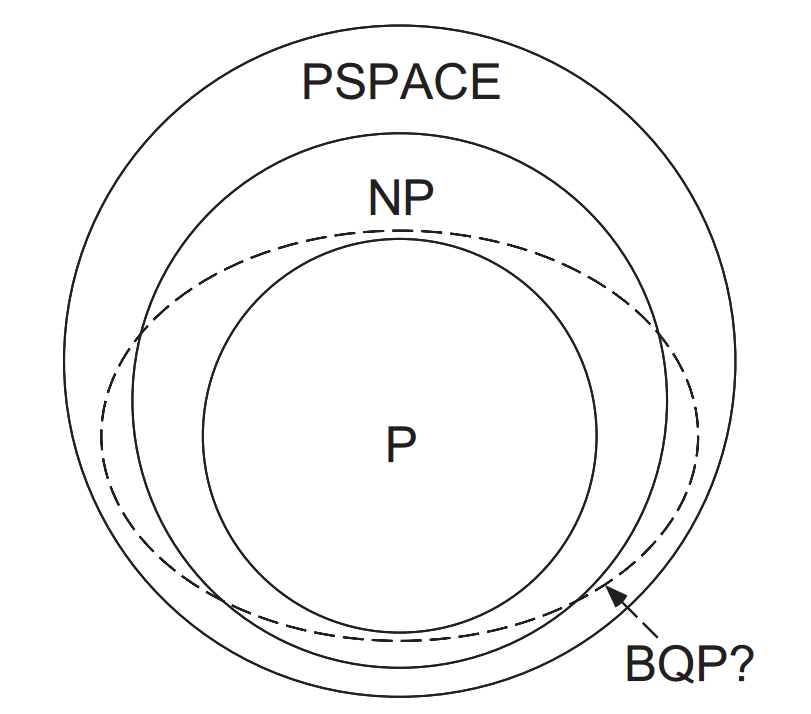
\includegraphics[scale=0.4]{classical_and_quantum_classes_relations}
\caption{The suspected relationship between the BQP and classical computational complexity classes.}
\end{figure}

\begin{definition}
Let's say, we are given an oracle returning a solution to a given problem (as previously, it does not have to be a correct solution). The \textbf{QMA} class (for \textbf{quantum Merlin Arthur}) is a set of problems, for which a solution given by the oracle can be verified by a quantum circuit in a polynomial time. The circuit has a probability of being correct greater than $\frac{2}{3}$.
\end{definition}

\begin{remark}
Although the BQP class is closer to the classical BPP class, we can see that relation between BQP and QMA is similar to the relation between P and NP. Because of this, these two classes are sometimes called as quantum equivalents of P and NP (BQP and QMA respectively).
\end{remark}


Final property of quantum computers, which will be discussed in this work, is their ability to speed up the process of finding solutions for problems from NP. The idea is, that we can generate each possible solution to a given problem, and then check each of them, whether it is correct or not (it is referred to as \textbf{brute force} method). Although, the amount of possible solutions for problems from NP is exponential, we will show in section \ref{quantum_search_algorithm}, that quantum computing provides a quadratic speed up in such a process.



	\cleardoublepage

	\chapter{Quantum circuits}
\thispagestyle{chapterBeginStyle}
\label{chapter2}

In the previous chapter we introduced a new concept called \textbf{quantum circuit}. In this chapter, we will describe it in detail, which will enable us to create algorithms, which will be presented in the next chapter.

\section{Qubits}

In classical computers information is stored using \textbf{bits}. These entities can be in two states - 0 or 1. Thanks to this, we can encode any information as a string of bits in appropriate states.

In the example \ref{example_0_1_states} from the previous chapter we introduced two vectors (states) - $|0\rangle = \begin{pmatrix} 1 \\ 0 \end{pmatrix}$ and $|1\rangle = \begin{pmatrix} 0 \\ 1 \end{pmatrix}$. These two states can be quantum equivalents of classical states 0 and 1. They are orthonormal
\[ \langle 0 | 1 \rangle = \begin{pmatrix} 1 & 0\end{pmatrix} \begin{pmatrix} 0 \\ 1 \end{pmatrix} = 1 \cdot 0 + 0 \cdot 1 = 0,\]
so they can create a basis for a vector in Hilbert space. Hence, such a vector can be represented as a combination of these two states
\[ |\psi \rangle = \alpha |0\rangle + \beta |1\rangle. \]

The above vector is the basic information unit in quantum computer science - \textbf{qubit}. Comparing to classical bit, which can be only in 2 states, qubit can be in an infinite number of states (because it can be in any combination of states $|0\rangle$ and $|1\rangle$). Such a vector can be represented on the \textbf{Bloch sphere} (given below).

\begin{figure}[ht]
\centering

\includegraphics[scale=0.1]{bloch_sphere}
\caption{Representation of a qubit on the Bloch sphere.}
\end{figure}

The Bloch sphere gives a convenient way to show properties of a state vector. We have written, that a qubit can be expressed as a combination $|\psi\rangle = \alpha |0\rangle + \beta|1\rangle$. We also have a normalization constraint $|\alpha|^2 + |\beta|^2 = 1$. If squares of two probability amplitudes give 1, we can replace them with \textit{sin} and \textit{cos} functions of the same angle. Moreover, we cannot measure a global phase of a vector, but just a local one. Such local phase can be written as $e^{i \phi}$, where $\phi$ is some angle. When we combine all of the above we get

\[ |\psi\rangle = cos\bigg( \frac{\Theta}{2}\bigg)|0\rangle + sin\bigg( \frac{\Theta}{2}\bigg) e^{i \phi}|1\rangle.\]

Angles $\Theta$ and $\phi$ are shown in the picture above. Change in any of these angles can be easily seen on a sphere, which would not be as simple in a coordinate system, where states $|0\rangle$ and $|1\rangle$ are perpendicular.


\section{Reversible circuits}

A classical circuit can be considered as a \textbf{reversible} taking into account two criteria - \textit{physical} and \textit{logical} reversibility. In this work we will discuss only the second one.

A \textit{logically reversible circuit} is a circuit, in which action of each logical gate can be undone. In other words, we can restore the state of each bit, before the gate was applied.

A simple, classical, one bit logic gate - \textbf{NOT} gate is fully reversible. Let's say, we have a bit in the state 0 and apply the NOT gate to it. We receive a bit in the state 1. But during the whole procedure we didn't lose any information about the previous state of the considered bit. We can reverse this operation by applying another NOT gate and change bit's state from 1 to 0 (a NOT gate is it's own inverse gate).

Now, let's consider a two bit \textbf{OR} gate. It implements a simple logical operation

\begin{table}[ht]
    \centering
    \begin{tabular}{c|c|c}
         A & B & $A \vee B$ \\
         0 & 0 & 0 \\
         0 & 1 & 1 \\
         1 & 0 & 1 \\
         1 & 1 & 1
    \end{tabular}
    \caption{The action of the OR gate.}
    \label{tab:or_gate_action}
\end{table}

We can see, that if we apply this gate to two bits and receive 0, it is obvious, that these bits were in state 0. But if we receive 1 as an output it is impossible to determine, which one of them was in the state 1 (both of them could also be in this state). In the computing process we lost some information about the initial state of our two bits.

Quantum circuit is a version of a reversible circuit. In fact, each logic gate used in a quantum circuit can be considered as an unitary operator (or an unitary matrix). Thanks to this, an action of each quantum gate can be undone by applying the inverse gate.

\begin{remark}
A quantum gate can be its own inverse gate. If matrix \textit{U} is its own inverse ($U \equiv U^\dagger$) and $UU^\dagger = \mathbb{1}$, it is called \textit{unitary} and \textit{Hermitian}.  
\end{remark}

\section{Representation of a quantum circuit}

Quantum circuits will be presented in the further part of this work in the following way:

\begin{itemize}
    \item The time evolution of a circuit will be associated with the horizontal axis. Because of this, left side of each schema of a circuit will be the beginning of the computation,
    \item Each qubit will have assigned a horizontal line. It will demonstrate the time evolution of the qubits state,
    \item Quantum gates will be presented in the form of boxes.
\end{itemize}

An example quantum circuit is presented below:

\[  \scalebox{2.0}{\Qcircuit @C=1em @R=1em {
\lstick{|\psi\rangle} & \gate{H} & \targ & \meter  \\
\lstick{|\phi\rangle} & \qw & \ctrl{-1} & \meter \\
\lstick{|\theta\rangle} & {/^{n}} \qw & \gate{X} & \meter
}} \]

We will now discuss only two of the occurring in the above circuit symbols (rest of them will be explained in detail in next sections).

The symbol given below symbolizes a measurement of a qubit

\[ \scalebox{2.5}{\Qcircuit @C=1em @R=1em {
& \meter & \rstick{} \cw
}} \]

Sometimes we will replace many lines representing time evolution of many qubits' states using the following notation


\[ \scalebox{2.5}{\Qcircuit @C=1em @R=1em {
& {/^{n}} \qw & \qw
}} \]


\section{Single qubit quantum gates}

In contrast to the classical model of computation, we can create infinitely many single qubit quantum gates (in classic case we could only use the \textit{NOT} gate on one bit). It is possible, because we can associate each quantum gate with a rotation of the quantum state on the Bloch sphere. It is obvious, that we can make infinitely many different rotations, which proves our statement.

Below is given notation for chosen single qubit quantum gates, which will be used in this work.

\paragraph{Identity gate}

\[ I = \begin{pmatrix} 1 & 0 \\ 0 & 1 \end{pmatrix} \]

\paragraph{Pauli X gate (NOT gate)}

\[ X = \begin{pmatrix} 0 & 1 \\ 1 & 0 \end{pmatrix} \]

\paragraph{Pauli Z gate}

\[ Z = \begin{pmatrix} 1 & 0 \\ 0 & -1 \end{pmatrix} \]

\paragraph{Hadamard gate}

\[ H =  \frac{1}{\sqrt{2}} \begin{pmatrix} 1 & 1 \\ 1 & -1 \end{pmatrix} \]

\paragraph{Phase shift ($R_k$ gate)}

\[ R_k = \begin{pmatrix} 1 & 0 \\ 0 & e^{\frac{2 \pi i}{2^k}} \end{pmatrix} \]

\begin{remark}
In literature the gate $R_k$ is often replaced with the $R_\phi$ gate, which is equivalent to

\[ R_\phi = \begin{pmatrix} 1 & 0 \\ 0 & e^{i \phi} \end{pmatrix}. \]

Despite this fact, we will use only the $R_k$ gate.
\end{remark}

\begin{remark}
As stated in the first chapter, when we are considering a complex physical system (made for example from two qubits) we are using the tensor product of the two component subsystems. Let's see this at the quantum circuit given below.

\[  \scalebox{2.0}{\Qcircuit @C=1em @R=1em {
\lstick{|\psi\rangle} & \gate{H} & \rstick{|\psi'\rangle} \qw \\
\lstick{|\phi\rangle} & \gate{I} & \rstick{|\phi'\rangle} \qw \\
}} \]

If we would like to replace the gates \textit{H} and \textit{I} with just one gate (let's call it \textit{C}) we would have to conduct the following procedure

\[ C = H \otimes I = \frac{1}{\sqrt{2}} \begin{pmatrix} 1 & 1 \\ 1 & -1 \end{pmatrix} \otimes \begin{pmatrix} 1 & 0 \\ 0 & 1\end{pmatrix} = \frac{1}{\sqrt{2}} \begin{pmatrix} 1 & 0 & 1 & 0 \\ 0 & 1 & 0 & 1 \\ 1 & 0 & -1 & 0 \\ 0 & 1 & 0 & -1 \end{pmatrix}.\]

We can see, that we can replace the \textit{C} gate with just \textbf{one layer} of smaller quantum gates. But it is not always possible. We will give an example of such a case in the next section.
\end{remark}

\section{Multiple qubit quantum gates}

In the first chapter we stated, that not all compound systems can be expressed in the form of tensor product of its subsystems. We called this phenomenon \textit{entanglement}. This property of quantum entities is often used in quantum computing. Using entanglement we can create \textbf{controlled gates}. A simple example of a controlled gate is the \textbf{controlled-NOT} gate (sometimes denoted as \textbf{CNOT}). In the matrix form it is written as

\[ CNOT = \begin{pmatrix} 1 & 0 & 0 & 0 \\ 0 & 1 & 0 & 0 \\ 0 & 0 & 0 & 1 \\ 0 & 0 & 1 & 0 \end{pmatrix} \]

We can see, that we cannot receive such a matrix as a result of tensor product of smaller matrices.

The \textit{CNOT} gate is represented in quantum circuits by the symbol

\[  \scalebox{2.0}{\Qcircuit @C=1em @R=1em {
 & \ctrl{1} & \qw \\
 & \targ & \qw \\
}} \]

The upper qubit is called a \textbf{control} qubit, and the bottom qubit is referred as to \textbf{target} qubit. To better understand what this quantum gate does, let's consider the following circuit

\[  \scalebox{2.0}{\Qcircuit @C=1em @R=1em {
\lstick{|\psi\rangle} & \ctrl{1} & \rstick{|\psi\rangle} \qw \\
\lstick{|\phi\rangle} & \targ & \rstick{|\phi \oplus \psi \rangle} \qw \\
}} \]

The \textit{CNOT} gate performs some operation (we will describe this operation in a moment), when the control qubit is in state $|1\rangle$. Otherwise, the whole system is left without any change.

In fact, the \textit{CNOT} gate can be understood as follows - it leaves the control qubit in the same state, and the bottom qubit becomes the result of \textit{addition modulo two} of the two qubits' states. Let's say, we have qubits in states $|0\rangle$ and $|1\rangle$ (accordingly control and target qubits). The usage of \textit{CNOT} gate can be written as

\[ CNOT |0\rangle \otimes |1\rangle = CNOT \begin{pmatrix} 1 \\ 0 \end{pmatrix} \otimes \begin{pmatrix} 0 \\ 1 \end{pmatrix} = \begin{pmatrix} 1 & 0 & 0 & 0 \\ 0 & 1 & 0 & 0 \\ 0 & 0 & 0 & 1 \\ 0 & 0 & 1 & 0 \end{pmatrix} \begin{pmatrix} 0 \\ 1 \\ 0 \\ 0 \end{pmatrix} = \begin{pmatrix} 0 \\ 1 \\ 0 \\ 0\end{pmatrix} = |0\rangle \otimes |1\rangle.\]

Now, let's consider qubits in states $|1\rangle$ and $|1\rangle$. The result of the above circuit for qubits in such states is equal to

\[ CNOT |1\rangle \otimes |1\rangle = CNOT \begin{pmatrix} 0 \\ 1 \end{pmatrix} \otimes \begin{pmatrix} 0 \\ 1 \end{pmatrix} = \begin{pmatrix} 1 & 0 & 0 & 0 \\ 0 & 1 & 0 & 0 \\ 0 & 0 & 0 & 1 \\ 0 & 0 & 1 & 0 \end{pmatrix} \begin{pmatrix} 0 \\ 0 \\ 0 \\ 1 \end{pmatrix} = \begin{pmatrix} 0 \\ 0 \\ 1 \\ 0 \end{pmatrix} = |1\rangle \otimes |0\rangle.\]

It is obvious, that $0 + 1 \ (mod \ 2) \equiv 1$ and $1 + 1 \ (mod \ 2) \equiv 0$, so we have shown, that understanding of the \textit{CNOT} gate in terms of the modular addition is correct. All possible results of the \textit{CNOT} gate are given in the table below.

\begin{table}[ht]
    \centering
    \begin{tabular}{c|c|c}
         $|\psi\rangle$ & $|\phi\rangle$ & $CNOT \  |\psi \phi \rangle$ \\ \hline
         $|0\rangle$ & $|0\rangle$ & $|00\rangle$ \\
         $|0\rangle$ & $|1\rangle$ & $|01\rangle$ \\
         $|1\rangle$ & $|0\rangle$ & $|11\rangle$ \\
         $|1\rangle$ & $|1\rangle$ & $|10\rangle$ \\
    \end{tabular}
    \caption{Actions of the \textit{CNOT} gate.}
    \label{tab:my_label}
\end{table}

The \textit{CNOT} gate is a simple extension of the \textit{NOT} gate. We can see, that the bottom right block of the \textit{CNOT} matrix is just the \textit{X} matrix. We can extend this reasoning, to create a whole class of controlled gates. Let's say, we have some quantum gate \textit{M} in the form

\[ M = \begin{pmatrix} m_{11} & m_{12} \\ m_{21} & m_{22}\end{pmatrix}. \]

The controlled version of this gate would have a form

\[ cM = \begin{pmatrix} 1 & 0 & 0 & 0 \\ 0 & 1 & 0 & 0 \\ 0 & 0 & m_{11} & m_{12} \\ 0 & 0 & m_{21} & m_{22} \end{pmatrix}. \]

Of course we can extend the simple case with a $2 \times 2$ matrix to a matrix with many inputs (acting on many qubits). Such a case will be represented by symbol

\[  \scalebox{1.5}{\Qcircuit @C=1em @R=.5em {
& \ctrl{1} & \qw \\
& \multigate{3}{M} & \qw \\
& \ghost{M} & \qw \\
& \ghost{M} & \qw \\
& \ghost{M} & \qw
}} \]

or 

\[  \scalebox{2.0}{\Qcircuit @C=1em @R=.5em {
& \qw & \ctrl{1} & \qw \\
& {/^{n}} \qw & \gate{M} & \qw 
}} \]

\begin{remark}
As we can see from the below calculations

\[ \begin{pmatrix} 1 & 0 & 0 & 0 \\ 0 & 1 & 0 & 0 \\ 0 & 0 & 0 & 1 \\ 0 & 0 & 1 & 0 \end{pmatrix} \begin{pmatrix} 1 & 0 & 0 & 0 \\ 0 & 1 & 0 & 0 \\ 0 & 0 & 0 & 1 \\ 0 & 0 & 1 & 0 \end{pmatrix} = \begin{pmatrix} 1 & 0 & 0 & 0 \\ 0 & 1 & 0 & 0 \\ 0 & 0 & 1 & 0 \\ 0 & 0 & 0 & 1 \end{pmatrix} \]

the \textit{CNOT} gate is its own inverse gate.
\end{remark}

Out of three \textit{CNOT} gates we can create a \textit{SWAP} gate, which changes states between two qubits. It will be denoted as 

\[  \scalebox{2.5}{\Qcircuit @C=1em @R=1em {
& \qswap & \qw \\
& \qswap \qwx & \qw
}} \]

\[ \]

and can be implemented with the following circuit

\[  \scalebox{2.0}{\Qcircuit @C=1em @R=.5em {
& \lstick{|\psi\rangle} & \ctrl{1} & \targ & \ctrl{1} & \qw & \rstick{|\phi\rangle}\\
& \lstick{|\phi\rangle} & \targ & \ctrl{-1} & \targ & \qw & \rstick{|\psi\rangle}
}} \]

Consecutive steps of the above construction can be written as

\[ |\psi, \phi \rangle \rightarrow |\psi, \phi \oplus \psi\rangle \] 
\[ \rightarrow |\psi \oplus (\phi \oplus \psi), \phi \oplus \psi\rangle \equiv |\phi, \phi \oplus \psi \rangle \]
\[ \rightarrow |\phi, (\phi \oplus \psi) \oplus \phi \rangle \equiv |\phi, \psi \rangle, \]
where coma was added to increase the readability of the whole procedure.

\section{Bell states} \label{bell_states}

Let's consider the following circuit:

\[  \scalebox{2.0}{\Qcircuit @C=1em @R=.5em {
& \lstick{|x\rangle} & \gate{H} & \ctrl{1} & \qw \\
& \lstick{|y\rangle} & \qw & \targ & \qw 
}} \]

Assuming, that $|x\rangle$ was only in one of $|0\rangle$ and $|1\rangle$ states, usage of the first Hadamrd gate has two possible outcomes:

\[ |0\rangle \xrightarrow{H} \frac{|0\rangle + |1\rangle}{\sqrt{2}}\]
\[ |1\rangle \xrightarrow{H} \frac{|0\rangle - |1\rangle}{\sqrt{2}}\]

As mentioned before, the \textit{CNOT} gate is applied to the $|y\rangle$ qubit only, if the control qubit is in a state $|1\rangle$. So, if we have a control qubit being in a superposition, the target qubit will also be in a superposition of being toggled and unchanged. Let's denote by $|\beta_{xy}\rangle$ state of the whole system after going through the whole circuit. We present possible values of $|\beta_{xy}\rangle$ in the table below.

\begin{table}[ht]
    \centering
    \begin{tabular}{|c|c|c|}
        \hline
         \multicolumn{2}{|c|}{Input} & Output \\ \hline
         $|x\rangle$ & $|y\rangle$ & $|\beta_{xy}\rangle$ \\ \hline
         $|0\rangle$ & $|0\rangle$ & $(|00\rangle + |11\rangle)/\sqrt{2}$ \\ \hline
         $|0\rangle$ & $|1\rangle$ & $(|01\rangle + |10\rangle)/\sqrt{2}$ \\ \hline
         $|1\rangle$ & $|0\rangle$ & $(|00\rangle - |11\rangle)/\sqrt{2}$ \\ \hline
         $|1\rangle$ & $|1\rangle$ & $(|01\rangle - |10\rangle)/\sqrt{2}$ \\ \hline
    \end{tabular}
    \caption{Bell states.}
\end{table}

Received $|\beta_{xy}\rangle$ states are called \textbf{Bell states}.


\section{Quantum gates with multiple control qubits, ancilla qubits}

We can extend the controlled gate model by adding more control qubits. The simplest example of quantum gate with many control qubits is the \textbf{Toffoli} gate. It will be denoted as

\[  \scalebox{2.0}{\Qcircuit @C=1em @R=1em {
& \lstick{|\psi\rangle} & \ctrl{2} & \qw & \rstick{|\psi\rangle}  \\
& \lstick{|\phi\rangle} & \ctrl{1} & \qw & \rstick{|\phi\rangle}  \\
& \lstick{|\theta\rangle} & \targ & \qw & \rstick{|\theta \oplus \psi\phi\rangle} 
}} \]
\[\]
It's action is similar to the one of the \textit{CNOT} gate. It applies addition modulo two on the target qubit, if two control qubits are in the state $|1\rangle$. It's effect is presented in the table below.

\begin{table}[ht]
    \centering
    \begin{tabular}{c|c}
         Input & Output \\ \hline
         $|000\rangle$ & $|000\rangle$ \\
         $|001\rangle$ & $|001\rangle$ \\
         $|010\rangle$ & $|010\rangle$ \\
         $|011\rangle$ & $|011\rangle$ \\
         $|100\rangle$ & $|100\rangle$ \\
         $|101\rangle$ & $|101\rangle$ \\
         $|110\rangle$ & $|111\rangle$ \\
         $|111\rangle$ & $|110\rangle$ \\
    \end{tabular}
    \caption{Actions of the Toffoli gate.}
    \label{tab:my_label}
\end{table}

It can be written in the matrix form as

\[ \begin{pmatrix} 1 & 0 & 0 & 0 & 0 & 0 & 0 & 0 \\ 0 & 1 & 0 & 0 & 0 & 0 & 0 & 0 \\ 0 & 0 & 1 & 0 & 0 & 0 & 0 & 0 \\ 0 & 0 & 0 & 1 & 0 & 0 & 0 & 0 \\ 0 & 0 & 0 & 0 & 1 & 0 & 0 & 0 \\ 0 & 0 & 0 & 0 & 0 & 1 & 0 & 0 \\ 0 & 0 & 0 & 0 & 0 & 0 & 0 & 1 \\ 0 & 0 & 0 & 0 & 0 & 0 & 1 & 0 \end{pmatrix}. \]


\begin{remark}
At this point we will assume, that it is physically possible to implement \textit{CNOT} and Toffoli gates. Because of this assumption, we can try to break down more complicated gates into \textit{CNOT} and Toffoli gates. Toffoli gates are in fact universal gates, which will be explained in the next section.
\end{remark}

Of course we can add next control qubits and receive for example such gate:

\[  \scalebox{2.0}{\Qcircuit @C=1em @R=1em {
 & \ctrl{4} & \qw \\
 & \ctrl{3} & \qw \\
 & \ctrl{2} & \qw \\
 & \ctrl{1} & \qw \\
 & \gate{M} & \qw \\
}} \]

\begin{remark}
\textit{NOT} gates with more than two control qubits will be denoted as $C^n NOT$ gates (where \textit{n} is the number of control qubits).
\end{remark}

Unfortunately, it might be physically impossible to construct such a gate. But, as we mentioned in the above remark, we can break it down into \textit{CNOT} and Toffoli gates. To achieve this goal we will have to use \textbf{ancilla qubits}.

\subsection{Ancilla qubits}

Ancilla qubits are additional qubits, which expand our work space. They can be, for example, taken from some other part of a quantum circuit, where they are currently not used. Because of this, it is sometimes necessary to return them in unchanged state to the original location in the circuit.

We will now introduce four types of ancilla qubits. Although this notation is not officially used (it was taken from \cite{craig_gidney}), we will use it, because it perfectly captures the nature of each ancilla qubit type.

\begin{itemize}
    \item \textbf{Burnable qubits} - initially, those qubits are in state $|0\rangle$ and there are no requirements about the state, in which it is to be found at the end of the computation.
    \item \textbf{Zeroed qubits} - initially they are in state $|0\rangle$ and have to be in this state, when we are not going to use them any more.
    \item \textbf{Garbage qubits} - the initial state of these qubits is unknown and there are no restrictions concerning the final state.
    \item \textbf{Borrowed qubits} - at the beginning of the computation they can be in any state and have to be returned in the same state.
\end{itemize}

\begin{remark}
We will use the following notation to denote different types of ancilla qubits:
\begin{itemize}
    \item $|BU_i\rangle$ for burnable qubits,
    \item $|Z_i\rangle$ for zeroed qubits,
    \item $|G_i\rangle$ for garbage qubits,
    \item $|BO_i\rangle$ for borrowed qubits,
\end{itemize}
where \textit{i} will be the index for the following ancilla qubits.
\end{remark}

\subsection{Decomposition of the $C^n NOT$ gate into $C^{n/2}NOT$ gates}

Our first goal is to break down the below gate into more gates with fewer control qubits.

\[  \scalebox{1.5}{\Qcircuit @C=1em @R=1em {
& \lstick{|a\rangle} & \ctrl{4} & \qw & \rstick{|a\rangle}  \\
& \lstick{|b\rangle} & \ctrl{3} & \qw & \rstick{|b\rangle}  \\
& \lstick{|c\rangle} & \ctrl{2} & \qw & \rstick{|c\rangle}  \\
& \lstick{|d\rangle} & \ctrl{1} & \qw & \rstick{|d\rangle}  \\
& \lstick{|T\rangle} & \targ & \qw & \rstick{|T \oplus abcd\rangle} 
}} \]

\paragraph{Decomposition of the $C^n NOT$ gate with one burnable qubit \\}

If we have one additional burnable qubit to use, we can toggle it, if half of the control qubits are in state $|1\rangle$. As a result we obtain the following circuit:

\[  \scalebox{1.5}{\Qcircuit @C=1em @R=1em {
& \lstick{|a\rangle} & \ctrl{4} & \qw & \qw & \rstick{|a\rangle}  \\
& \lstick{|b\rangle} & \ctrl{3} & \qw & \qw & \rstick{|b\rangle}  \\
& \lstick{|c\rangle} & \qw & \ctrl{3} & \qw & \rstick{|c\rangle}  \\
& \lstick{|d\rangle} & \qw & \ctrl{2} & \qw & \rstick{|d\rangle}  \\
& \lstick{|BU_1\rangle} & \targ & \ctrl{1} & \qw & \rstick{|0 \oplus ab\rangle = |ab\rangle}  \\
& \lstick{|T\rangle} & \qw & \targ & \qw & \rstick{|T \oplus abcd\rangle} 
}} \]

\paragraph{Decomposition of the $C^n NOT$ gate with one zeroed qubit \\}

At the end of the previous section we have shown, that the \textit{CNOT} gate is its own inverse gate. In fact, any $C^nNOT$ gate is its own inverse gate. We will use this property, while using the \textit{zeroed} qubit. If we apply the $C^nNOT$ gate to this ancilla qubit for the first time, its state might change. But we can cancel the action of the first gate by using the $C^nNOT$ gate second time. This reasoning gives us the following quantum circuit:

\[  \scalebox{1.5}{\Qcircuit @C=1em @R=1em {
& \lstick{|a\rangle} & \ctrl{4} & \qw & \ctrl{4} & \qw & \rstick{|a\rangle}  \\
& \lstick{|b\rangle} & \ctrl{3} & \qw & \ctrl{3} & \qw & \rstick{|b\rangle}  \\
& \lstick{|c\rangle} & \qw & \ctrl{3} & \qw & \qw & \rstick{|c\rangle}  \\
& \lstick{|d\rangle} & \qw & \ctrl{2} & \qw & \qw & \rstick{|d\rangle}  \\
& \lstick{|Z_1\rangle} & \targ & \ctrl{1} &\targ & \qw & \rstick{|Z_1\rangle = |0\rangle}  \\
& \lstick{|T\rangle} & \qw & \targ & \qw & \qw & \rstick{|T \oplus abcd\rangle} 
}} \]

\paragraph{Decomposition of the $C^n NOT$ gate with one garbage qubit \\}

Because we do not know the initial state of the garbage qubit, the only way for us do detect any behavior is to check, whether it was toggled or not. The \textit{modular addition} (or \textit{XOR} operation) has such property, that if we use it two times with the same argument, these operations cancel out. This can be written as

\[ x \oplus y \oplus y \equiv x.  \]

This property gives us the following structure

\[  \scalebox{1.5}{\Qcircuit @C=1em @R=1em {
& \lstick{|a\rangle} & \qw & \ctrl{4} & \qw & \qw & \rstick{|a\rangle}  \\
& \lstick{|b\rangle} & \qw & \ctrl{3} & \qw & \qw & \rstick{|b\rangle}  \\
& \lstick{|c\rangle} & \ctrl{3} & \qw & \ctrl{3} & \qw & \rstick{|c\rangle}  \\
& \lstick{|d\rangle} & \ctrl{2} & \qw & \ctrl{2} & \qw & \rstick{|d\rangle}  \\
& \lstick{|G_1\rangle} & \ctrl{1} &\targ & \ctrl{1} & \qw & \rstick{|G_1 \oplus ab \rangle}  \\
& \lstick{|T\rangle} & \targ & \qw & \targ & \qw & \rstick{|T \oplus abcd\rangle} 
}} \]

We can see, that we are adding $|G_1\rangle$ to $|T\rangle$ two times, so these operations cancel out. The only possible leftover of this procedure is $|T \oplus ab\rangle$. Finally, the result of the whole above circuit can be written as

\[ |T \oplus G_1cd \oplus (G_1 \oplus ab)cd \rangle \equiv |T \oplus (G_1 \oplus G_1 \oplus ab)cd \rangle \equiv |T \oplus abcd \rangle\]

\paragraph{Decomposition of the $C^n NOT$ gate with one borrowed qubit \\}

The last case is very similar to the previous one (with garbage qubit). We only have to detect the possible toggling of the borrowed qubit and moreover, we have to undo the operation applied on it, to restore it to its initial state. It can be done using the below circuit

\[  \scalebox{1.5}{\Qcircuit @C=1em @R=1em {
& \lstick{|a\rangle} & \ctrl{4} & \qw & \ctrl{4} & \qw & \qw & \rstick{|a\rangle}  \\
& \lstick{|b\rangle} & \ctrl{3} & \qw & \ctrl{3} & \qw & \qw & \rstick{|b\rangle}  \\
& \lstick{|c\rangle} & \qw & \ctrl{3} & \qw & \ctrl{3} & \qw & \rstick{|c\rangle}  \\
& \lstick{|d\rangle} & \qw & \ctrl{2} & \qw & \ctrl{2} & \qw & \rstick{|d\rangle}  \\
& \lstick{|BO_1\rangle} & \targ & \ctrl{1} &\targ & \ctrl{1} & \qw & \rstick{|BO_1\rangle}  \\
& \lstick{|T\rangle} & \qw & \targ & \qw & \targ & \qw & \rstick{|T \oplus abcd\rangle} 
}} \]

\subsection{Decomposition of the $C^nNOT$ gate using \textit{n - 2} ancilla qubits}

We stated in the previous section, that it is possible to physically implement Toffoli gates. We will now try to break down $C^nNOT$ gate using different types of ancilla qubits and Toffoli gates.

In presented circuits we will interleave basic and ancilla qubits in order to increase the readability of diagrams. We will use constructions derived in the previous subsection and only show diagrams representing decomposed $C^nNOTs$.

\paragraph{Decomposition of the $C^nNOT$ gate using burnable qubits\\}

\[ \scalebox{1.3}{\Qcircuit @C=1em @R=1em {
& \lstick{|a\rangle} & \ctrl{2} & \qw & \qw & \qw & \qw & \rstick{|a\rangle} \\
& \lstick{|b\rangle} & \ctrl{1} & \qw & \qw & \qw & \qw & \rstick{|b\rangle} \\
& \lstick{|BU_1\rangle} & \targ & \ctrl{2} & \qw & \qw & \qw & \rstick{|ab\rangle} \\
& \lstick{|c\rangle} & \qw & \ctrl{1} & \qw & \qw & \qw & \rstick{|c\rangle} \\
& \lstick{|BU_2\rangle} & \qw & \targ & \ctrl{2} & \qw & \qw & \rstick{|abc\rangle} \\
& \lstick{|d\rangle} & \qw & \qw & \ctrl{1} & \qw & \qw & \rstick{|d\rangle} \\
& \lstick{|BU_3\rangle} & \qw & \qw & \targ & \ctrl{2} & \qw & \rstick{|abcd\rangle} \\
& \lstick{|e\rangle} & \qw & \qw & \qw & \ctrl{1} & \qw & \rstick{|e\rangle} \\
& \lstick{|T\rangle} & \qw & \qw & \qw & \targ & \qw & \rstick{|T \oplus abcde\rangle} 
}} \]

\paragraph{Decomposition of the $C^nNOT$ gate using zeroed qubits\\}

\[ \scalebox{1.3}{\Qcircuit @C=1em @R=1em {
&\lstick{|a\rangle} & \ctrl{2} & \qw & \qw & \qw & \qw & \qw & \ctrl{2} & \qw & \rstick{|a\rangle} \\
& \lstick{|b\rangle} & \ctrl{1} & \qw & \qw & \qw & \qw & \qw & \ctrl{1} & \qw & \rstick{|b\rangle} \\
& \lstick{|Z_1\rangle} & \targ & \ctrl{2} & \qw & \qw & \qw & \ctrl{2} & \targ & \qw &  \rstick{|Z_1\rangle = |0\rangle} \\
& \lstick{|c\rangle} & \qw & \ctrl{1} & \qw & \qw & \qw & \ctrl{1} & \qw & \qw & \rstick{|c\rangle} \\
& \lstick{|Z_2\rangle} & \qw & \targ & \ctrl{2} & \qw & \ctrl{2} & \targ & \qw& \qw &  \rstick{|Z_2\rangle = |0\rangle} \\
& \lstick{|d\rangle} & \qw & \qw & \ctrl{1} & \qw & \ctrl{1} & \qw & \qw & \qw & \rstick{|d\rangle} \\
& \lstick{|Z_3\rangle} & \qw & \qw & \targ & \ctrl{2} & \targ & \qw & \qw & \qw &  \rstick{|Z_3\rangle = |0\rangle} \\
& \lstick{|e\rangle} & \qw & \qw & \qw & \ctrl{1} & \qw & \qw & \qw & \qw & \rstick{|e\rangle} \\
& \lstick{|T\rangle} & \qw & \qw & \qw & \targ  & \qw & \qw & \qw & \qw & \rstick{|T \oplus abcde\rangle} 
}} \]

\paragraph{Decomposition of the $C^nNOT$ gate using garbage qubits\\}

\[ \scalebox{1.3}{\Qcircuit @C=1em @R=1em {
& \lstick{|a\rangle} & \qw & \qw & \qw & \qw & \ctrl{2} & \qw & \qw & \qw & \qw & \rstick{|a\rangle} \\
& \lstick{|b\rangle} & \qw & \qw & \qw & \qw & \ctrl{1} & \qw & \qw & \qw & \qw & \rstick{|b\rangle} \\
& \lstick{|G_1\rangle} & \qw & \qw & \qw & \ctrl{2} & \targ & \ctrl{2} & \qw & \qw & \qw & \rstick{|G_1 \oplus ab\rangle} \\
& \lstick{|c\rangle} & \qw & \qw & \qw & \ctrl{1} & \qw & \ctrl{1} & \qw & \qw & \qw & \rstick{|c\rangle} \\
& \lstick{|G_2\rangle} & \qw & \qw & \ctrl{2} & \targ & \qw & \targ & \ctrl{2} & \qw & \qw & \rstick{|G_2 \oplus abc\rangle} \\
& \lstick{|d\rangle} & \qw & \qw & \ctrl{1} & \qw & \qw & \qw & \ctrl{1} & \qw & \qw & \rstick{|d\rangle} \\
& \lstick{|G_3\rangle} & \qw & \ctrl{2} & \targ & \qw & \qw & \qw & \targ & \ctrl{2} & \qw & \rstick{|G_3 \oplus abcd\rangle} \\
& \lstick{|e\rangle} & \qw & \ctrl{1} & \qw & \qw & \qw & \qw & \qw & \ctrl{1} & \qw & \rstick{|e\rangle} \\
& \lstick{|T\rangle} & \qw & \targ & \qw & \qw & \qw & \qw & \qw & \targ & \qw & \rstick{|T \oplus abcde \rangle} \\
}} \]

\paragraph{Decomposition of the $C^nNOT$ gate using borrowed qubits\\}

\[ \scalebox{1.3}{\Qcircuit @C=1em @R=1em {
& \lstick{|a\rangle} & \qw & \qw & \qw & \qw & \ctrl{2} & \qw & \qw & \qw & \qw & \qw & \ctrl{2} & \qw & \qw & \qw & \rstick{|a\rangle} \\
& \lstick{|b\rangle} & \qw & \qw & \qw & \qw & \ctrl{1} & \qw & \qw & \qw & \qw & \qw & \ctrl{1} & \qw & \qw & \qw & \rstick{|b\rangle} \\
& \lstick{|BO_1\rangle} & \qw & \qw & \qw & \ctrl{2} & \targ & \ctrl{2} & \qw & \qw & \qw & \ctrl{2} & \targ & \ctrl{2} & \qw & \qw & \rstick{|BO_1\rangle} \\
& \lstick{|c\rangle} & \qw & \qw & \qw & \ctrl{1} & \qw & \ctrl{1} & \qw & \qw & \qw & \ctrl{1} & \qw & \ctrl{1} & \qw & \qw & \rstick{|c\rangle} \\
& \lstick{|BO_2\rangle} & \qw & \qw & \ctrl{2} & \targ & \qw & \targ & \ctrl{2} & \qw & \ctrl{2} & \targ & \qw & \targ & \ctrl{2} & \qw & \rstick{|BO_2\rangle} \\
& \lstick{|d\rangle} & \qw & \qw & \ctrl{1} & \qw & \qw & \qw & \ctrl{1} & \qw & \ctrl{1} & \qw & \qw & \qw & \ctrl{1} & \qw & \rstick{|d\rangle} \\
& \lstick{|BO_3\rangle} & \qw & \ctrl{2} & \targ & \qw & \qw & \qw & \targ & \ctrl{2} & \targ & \qw & \qw & \qw & \targ & \qw & \rstick{|BO_3\rangle} \\
& \lstick{|e\rangle} & \qw & \ctrl{1} & \qw & \qw & \qw & \qw & \qw & \ctrl{1} & \qw & \qw & \qw & \qw & \qw & \qw & \rstick{|e\rangle} \\
& \lstick{|T\rangle} & \qw & \targ & \qw & \qw & \qw & \qw & \qw & \targ & \qw & \qw & \qw & \qw & \qw & \qw & \rstick{|T \oplus abcde\rangle} \\
}} \]

\subsection{Decomposition of the $C^nNOT$ gate using \textit{O(n)} Toffoli gates and ancilla qubits}

Our final goal in this section is to decompose the $C^nNOT$ gate into Toffoli and \textit{NOT} gates. First of all let us explain, why it is sometimes impossible without using ancilla qubits (only, when we are considering reversible circuits, but not the quantum ones).

We can understand the action of a $C^nNOT$ gate as kind of permutation. Let's consider a four-qubit circuit. A $C^3NOT$ gate (given in the picture below) flips the state of the last qubit, if all of the previous ones are in the $|1\rangle$ state (it changes the $|111\psi\rangle$ state into $|111\bar{\psi}\rangle$, where $|\bar{\psi}\rangle$ is a negation of the $|\psi\rangle$ state). We can say, that this gate performs a swap operation only on one position (on the last index, which represents the last qubit). Because it does only one swap, it has an \textit{odd} parity (or the number of states, on which it performs a swap is equal to one, and therefore odd).

\[ \scalebox{1.5}{\Qcircuit @C=1em @R=1em {
& \lstick{|a\rangle} & \qw & \ctrl{3} & \qw & \rstick{|a\rangle} \\
& \lstick{|b\rangle} & \qw & \ctrl{2} & \qw & \rstick{|b\rangle} \\
& \lstick{|c\rangle} & \qw & \ctrl{1} & \qw & \rstick{|c\rangle} \\
& \lstick{|d\rangle} & \qw & \targ & \qw & \rstick{|d \oplus abc\rangle} \\
}} \]

Now let's consider the $C^2NOT$ (or the Toffoli gate) on the same circuit. 

\[ \scalebox{1.5}{\Qcircuit @C=1em @R=1em {
& \lstick{|a\rangle} & \qw & \ctrl{2} & \qw & \rstick{|a\rangle} \\
& \lstick{|b\rangle} & \qw & \ctrl{1} & \qw & \rstick{|b\rangle} \\
& \lstick{|c\rangle} & \qw & \targ & \qw & \rstick{|c \oplus ab\rangle} \\
& \lstick{|d\rangle} & \qw & \qw & \qw & \rstick{|d\rangle} \\
}} \]

\[\]

It does not affect the last qubit in any way during the computation. Because of this we can say, that it performs swap on the third qubit in two states: $|11\psi0\rangle$ and $|11\psi1\rangle$, so it has an \textit{even} parity.

If we would like to create larger gates out of chained layers of smaller ones, we would add parities of all layers to make sure, that their parity matches the parity of the target gate. This observation leads us to the conclusion, that it is impossible to create gates with odd parity out of gates with even parity. In such a case we are forced to use ancilla qubits.

\begin{remark}
As we mentioned before, the above conclusion applies only to reversible circuits, but not to quantum ones. It is possible to decompose multiply-controlled quantum gates into smaller ones without any ancilla qubits, but this topic will not be discussed in this work. The purpose of this section and given examples is to tame the reader with ancilla qubits (which will be used in algorithms presented in the next chapter) and the process of decomposition of gates.
\end{remark}

We will now present the decomposition of the $C^5NOT$ using Toffoli gates (we stated earlier, that these are universal gates). Regarding the above conclusion, we are forced to use ancilla qubits to achieve this goal.

We will begin with using only one borrowed qubit. Moreover, we will use initial qubits as ancilla qubits for the Toffoli gates (they will be also treated as borrowed qubits). Having all this in mind, we obtain the following circuit (note, that the position of ancilla and target qubit are flipped compared with the previous circuits):

\begin{table}[ht]
\centering
\begin{tikzpicture}
\node (a) at (-40,0){
\scalebox{1.5}{\Qcircuit @C=1em @R=1em {
& \lstick{|a\rangle} & \ctrl{5} & \qw  \\
& \lstick{|b\rangle} & \ctrl{4} & \qw  \\
& \lstick{|c\rangle} & \ctrl{3} & \qw  \\
& \lstick{|d\rangle} & \ctrl{2} & \qw  \\
& \lstick{|e\rangle} & \ctrl{1} & \qw  \\
& \lstick{|T\rangle} & \targ & \qw  \\
& \lstick{|BO_1\rangle} & \qw & \qw
}}
};
\node[xshift=3.5cm] (b) at (a.east) 
{
\scalebox{1.5}{\Qcircuit @C=1em @R=1em {
& \ctrl{6} & \qw & \ctrl{6} & \qw & \qw  \\
& \qw & \ctrl{4} & \qw & \ctrl{4} & \qw \\
& \ctrl{4} & \qw & \ctrl{4} & \qw & \qw \\
& \qw & \ctrl{2} & \qw & \ctrl{2} & \qw \\
& \ctrl{2} & \qw & \ctrl{2} & \qw & \qw \\
& \qw & \targ & \qw & \targ & \qw \\
& \targ & \ctrl{-1} & \targ & \ctrl{-1} & \qw
}}
};
\draw[->,ultra thick](a)--(b);
\node[xshift=1.5cm] (c) at (b.east) 
{};
\draw[->,ultra thick](b)--(c);
\end{tikzpicture}
\label{my-label}
\end{table}

\Qcircuit @C=1em @R=1em {
& \qw & \qw & \ctrl{3} & \qw & \qw & \qw & \ctrl{3} & \qw & \qw & \qw & \qw & \qw & \qw & \qw & \ctrl{3} & \qw & \qw & \qw & \ctrl{3} & \qw & \qw & \qw & \qw & \qw & \qw \\ 
& \qw & \qw & \qw & \qw & \qw & \qw & \qw & \qw & \qw & \ctrl{3} & \qw & \ctrl{3} & \qw & \qw & \qw & \qw & \qw & \qw & \qw & \qw & \qw & \ctrl{3} & \qw & \ctrl{3} & \qw \\ 
& \qw & \qw & \ctrl{1} & \qw & \qw & \qw & \ctrl{1} & \qw & \qw & \qw & \qw & \qw & \qw & \qw & \ctrl{1} & \qw & \qw & \qw & \ctrl{1} & \qw & \qw & \qw & \qw & \qw & \qw \\ 
& \qw & \ctrl{2} & \targ & \ctrl{2} & \qw & \ctrl{2} & \targ & \ctrl{2} & \qw & \ctrl{1} & \qw & \ctrl{1} & \qw & \ctrl{2} & \targ & \ctrl{2} & \qw & \ctrl{2} & \targ & \ctrl{2} & \qw & \ctrl{1} & \qw & \ctrl{1} & \qw \\ 
& \qw & \ctrl{1} & \qw & \ctrl{1} & \qw & \ctrl{1} & \qw & \ctrl{1} & \ctrl{1} & \targ & \ctrl{1} & \targ & \qw & \ctrl{1} & \qw & \ctrl{1} & \qw & \ctrl{1} & \qw & \ctrl{1} & \ctrl{1} & \targ & \ctrl{1} & \targ & \qw \\ 
& \ctrl{1} & \targ & \qw & \targ & \ctrl{1} & \targ & \qw & \targ & \targ & \qw & \targ & \qw & \ctrl{1} & \targ & \qw & \targ & \ctrl{1} & \targ & \qw & \targ & \targ & \qw & \targ & \qw & \qw \\ 
& \targ & \qw & \qw & \qw & \targ & \qw & \qw & \qw & \ctrl{-1} & \qw & \ctrl{-1} & \qw & \targ & \qw & \qw & \qw & \targ & \qw & \qw & \qw & \ctrl{-1} & \qw & \ctrl{-1} & \qw & \qw \\ 
}

\[ \]

For \textit{n} equal to \textit{5} we achieved the circuit consisting of \textit{24} gates. In general case, we would need about \textit{16n} gates (using one borrowed qubit) which gives us desired \textit{O(n)} bound. We also have lower bound $\Omega(n)$, because with smaller amount of Toffoli gates we would be unable to touch all of the qubits. These bounds combined give us the $\Theta(n)$ complexity of the final circuit. The constant factor, which stands by \textit{n}, depends on the number and type of ancilla qubits which we can use. If we would have one burnable qubit instead of borrowed one we would reduce this number from \textit{16} to about \textit{8}. On the other hand, if we would have \textit{n} borrowed qubits, we would reduce this factor further, down to about \textit{4}. Using \textit{n} zeroed of garbage qubits would give us the circuit of the size about \textit{2n}. Finally, if we were given \textit{n} burnable qubits we would need only \textit{n} elementary gates.


\section{Universal quantum gates} \label{elementary_quantum_gates}

A set of gates, which can implement arbitrary quantum gates will be called \textit{universal}. At the beginning it is important to notice, that a set of all possible quantum gates is \textbf{uncountable}. A set of possible states, in which a qubit can be is comparable to the set of real numbers (between any two quantum states we can always find a new one). On the other hand, a set of finite sequences made from elements from a finite set is \textbf{countable}. We will deal with this problem by assuming, that we can approximate any quantum gate with arbitrary precision.

First set of universal quantum gates is a set consisting of the \textbf{\textit{CNOT}} gate, \textbf{Hadamard} gate and the $\mathbf{R_3}$ gate ($R_3 \equiv \begin{pmatrix} 1 & 0 \\ 0 & e^{\frac{i \pi}{4}}\end{pmatrix}$).

The second set of universal gates consists only of the \textbf{Toffoli} gate.

There are other sets of universal quantum gates, but we presented only the above two to not confuse the reader with information, which will not be used in the further part of this work.
	\cleardoublepage
	
	\chapter{Quantum algorithms}
\thispagestyle{chapterBeginStyle}
\label{chapter3}

In this chapter we are going to present three main applications of quantum computers: quantum search, algorithms based on quantum Fourier transform and simulations of Hamiltonians. We will show the implementation of Grover's and Shors's algorithms as examples from the first two categories. Finally, we will show simple quantum circuit (although not created out of elementary gates), which can simulate behavior of a simple physical system.

\section{Quantum search algorithm}\label{quantum_search_algorithm}

Let's consider a simple scenario, in which we would like to store 2-bit numbers in a classic database. To achieve this goal, we would need separate bits for each saved number. For example, if we would like to store all possible 2-bit numbers 00, 01, 10, 11, we would need 8 bits in total. At the same time, we could store all of the states $|00\rangle$, $|01\rangle$, $|10\rangle$, $|11\rangle$ on only 2 qubits. We would just assign the same probability to each of these states (obtain uniform superposition):

\[ |s\rangle = \frac{1}{2}|00\rangle + \frac{1}{2}|01\rangle + \frac{1}{2}|10\rangle + \frac{1}{2}|11\rangle\]

(during the measurement we get the square of the factor next to the state, to which the system collapses, so we have a $\frac{1}{4}$ probability of obtaining each of the elementary states). The initial state for our algorithm will be exactly this uniform superposition: $|\psi_0\rangle = |s\rangle$. It can be obtained by applying Hadamard gate to each qubit, which is denoted as $H^{\otimes n}$ (where \textit{n} is a number of qubits).

Now let's say, that we are searching for a number $|w\rangle$ in our quantum database. In that case, we can represent our superposition as a vector in space spanned by vectors $|w\rangle$ and $|s'\rangle$ (the latter one is just an orthonormal vector to the vector $|w\rangle$).

\begin{figure}[ht]
\centering
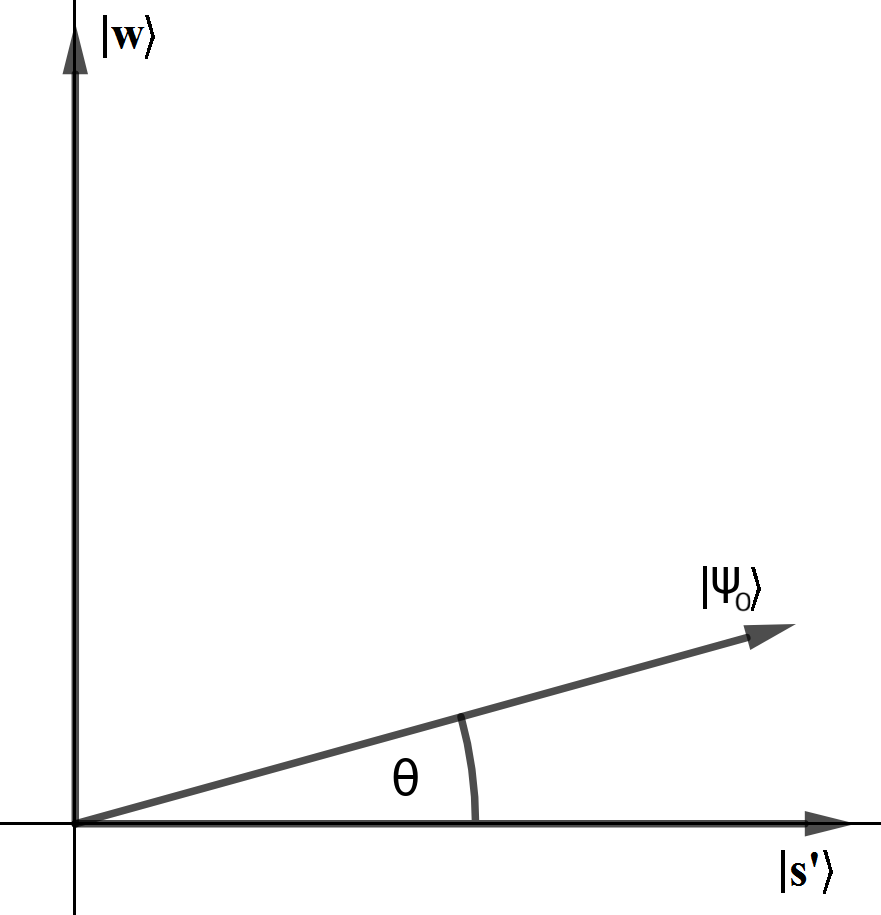
\includegraphics[scale=0.25]{grover_1}
\caption{Representation of the uniform superposition of stored numbers as a vector.}
\end{figure}

As mentioned earlier $|\psi_0\rangle$ is a uniform superposition, so $|w\rangle$ vector is one of its components. Due to this, $|\psi_0\rangle$ cannot be perpendicular to the $|w\rangle$ vector, but it also has to be above the $|s'\rangle$ (because it has to be between these two basis vectors). The initial state $|\psi_0\rangle$ can be also shown on a bar diagram:

\begin{figure}[ht]
\centering
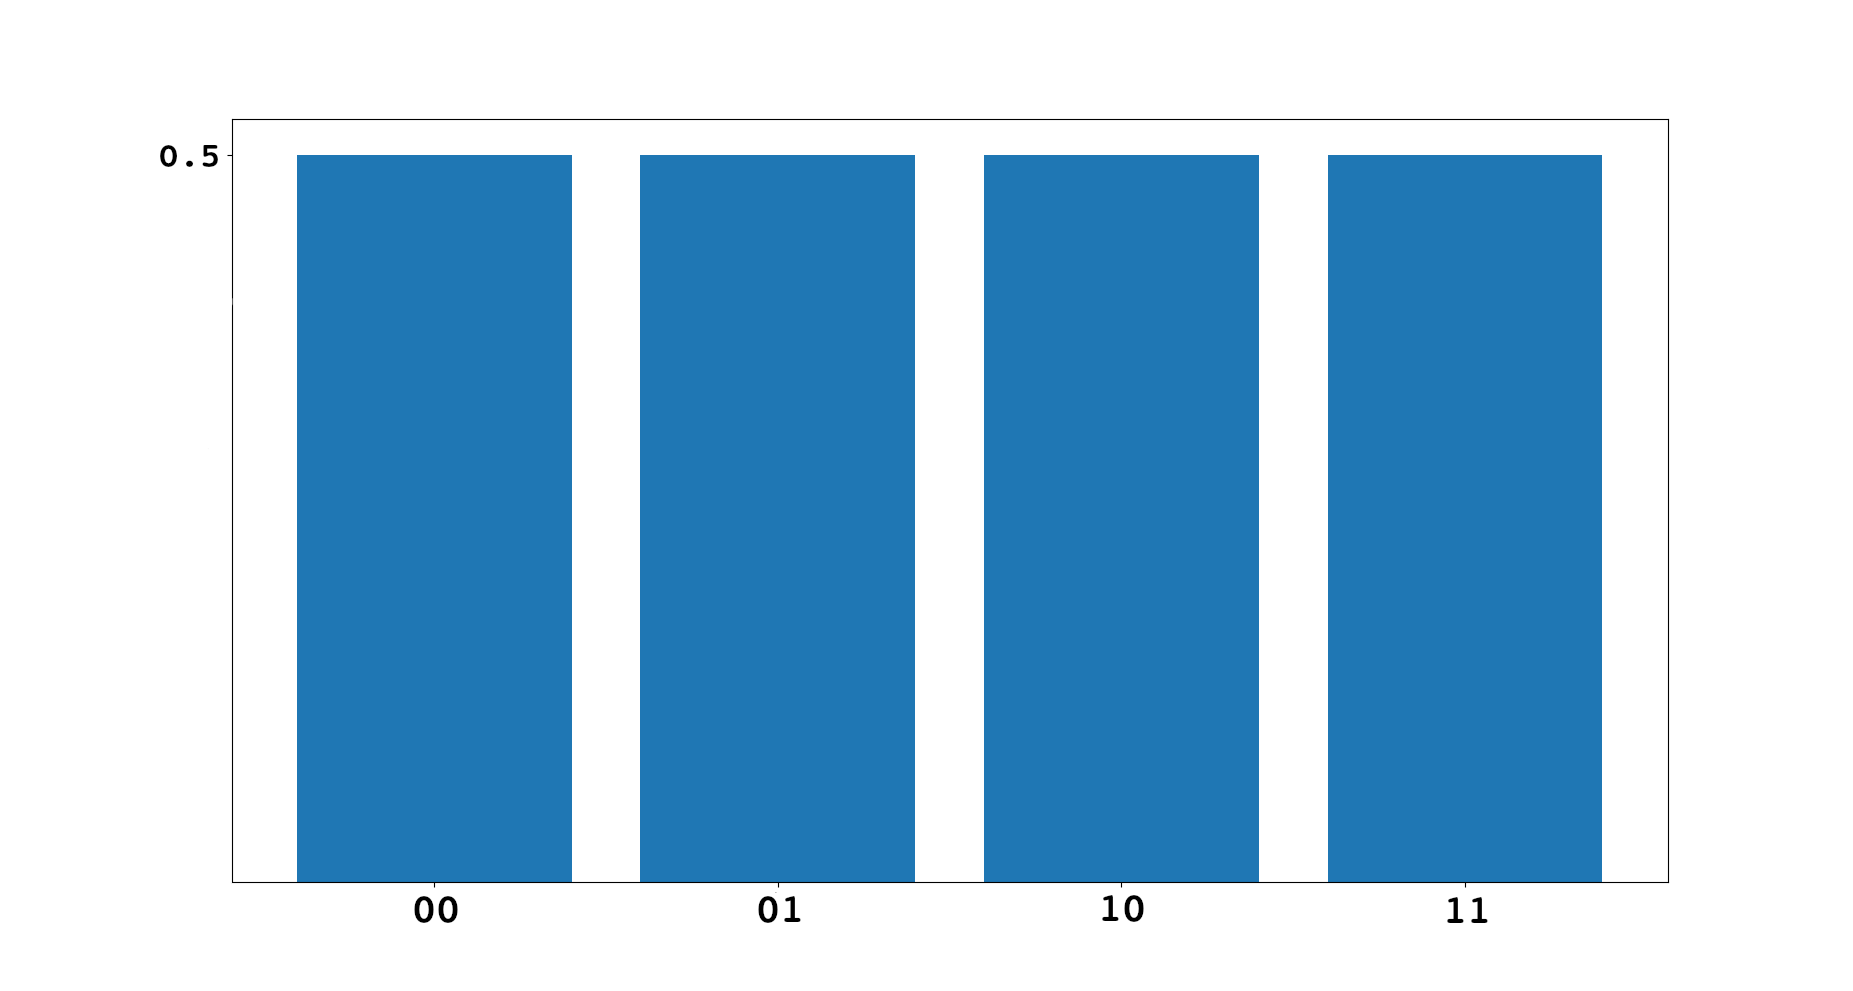
\includegraphics[scale=0.25]{grover_bars_1}
\caption{The uniform superposition presented on a bar diagram.}
\end{figure}

Let's denote the factors standing next to the states as $c_i$ (where \textit{i} is the index of a state or number, which is stored in it).

Before going further, we need to introduce another assumption. We claim, that we are in possession of a function (given for example by an oracle) which recognizes the number $w$. It will be denoted as

\[ f(x) = \begin{cases}
        0, & if\  x \neq w \\
        1, & if\  x = w
        \end{cases} \]

We are also going to introduce an operator, which uses the above function. It also can be understood as an extension of this function

\[ U_f|x\rangle = \begin{cases}
        |x\rangle, & if\  |x\rangle \neq |w\rangle \\
        -|x\rangle, & if\  |x\rangle = |w\rangle,
        \end{cases} \]

which can be rewritten as 

\[ U_f|x\rangle = (-1)^{f(x)}|x\rangle. \]

Of course we can see, that $U_f|w\rangle = -|w\rangle$.

\begin{remark}
Operator $U_f$ can act differently, than just recognizing a specific number. Another example of it is an operator recognizing numbers divisible by 2.
\end{remark}

Let's say, we are looking for a number 2 in our quantum database. If we apply the $U_f$ operator to our initial state $|\psi_0\rangle$ the factor $c_2$ will become negative, which is shown at the bar diagram below:

\begin{figure}[ht]
\centering
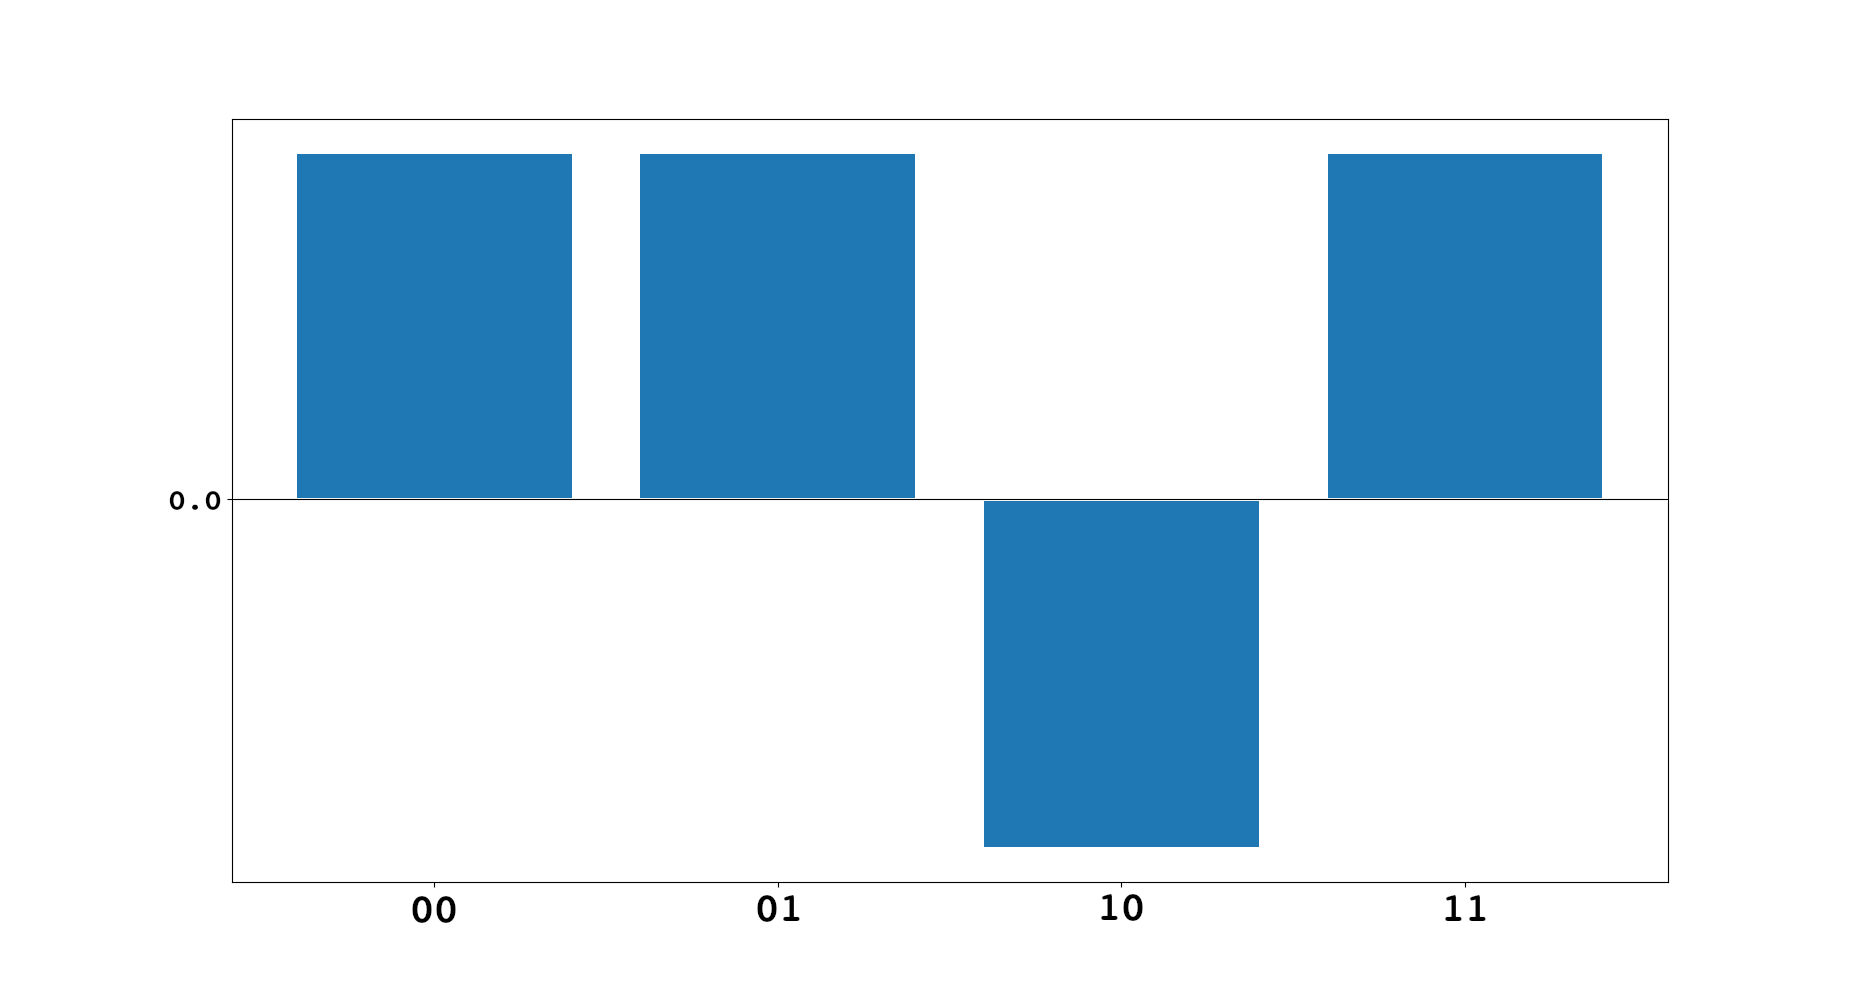
\includegraphics[scale=0.25]{grover_bars_2.png}
\caption{Bar diagram of the vector $U_f|\psi_0\rangle$.}
\end{figure}

\newpage
(this factor can be negative, because during the measurement we will obtain a square of it). The action of the $U_f$ operator can be also understood as a rotation of the vector $|\psi_0\rangle$ along the axis, on which lies the basis vector $|s'\rangle$:

\begin{figure}[ht]
\centering
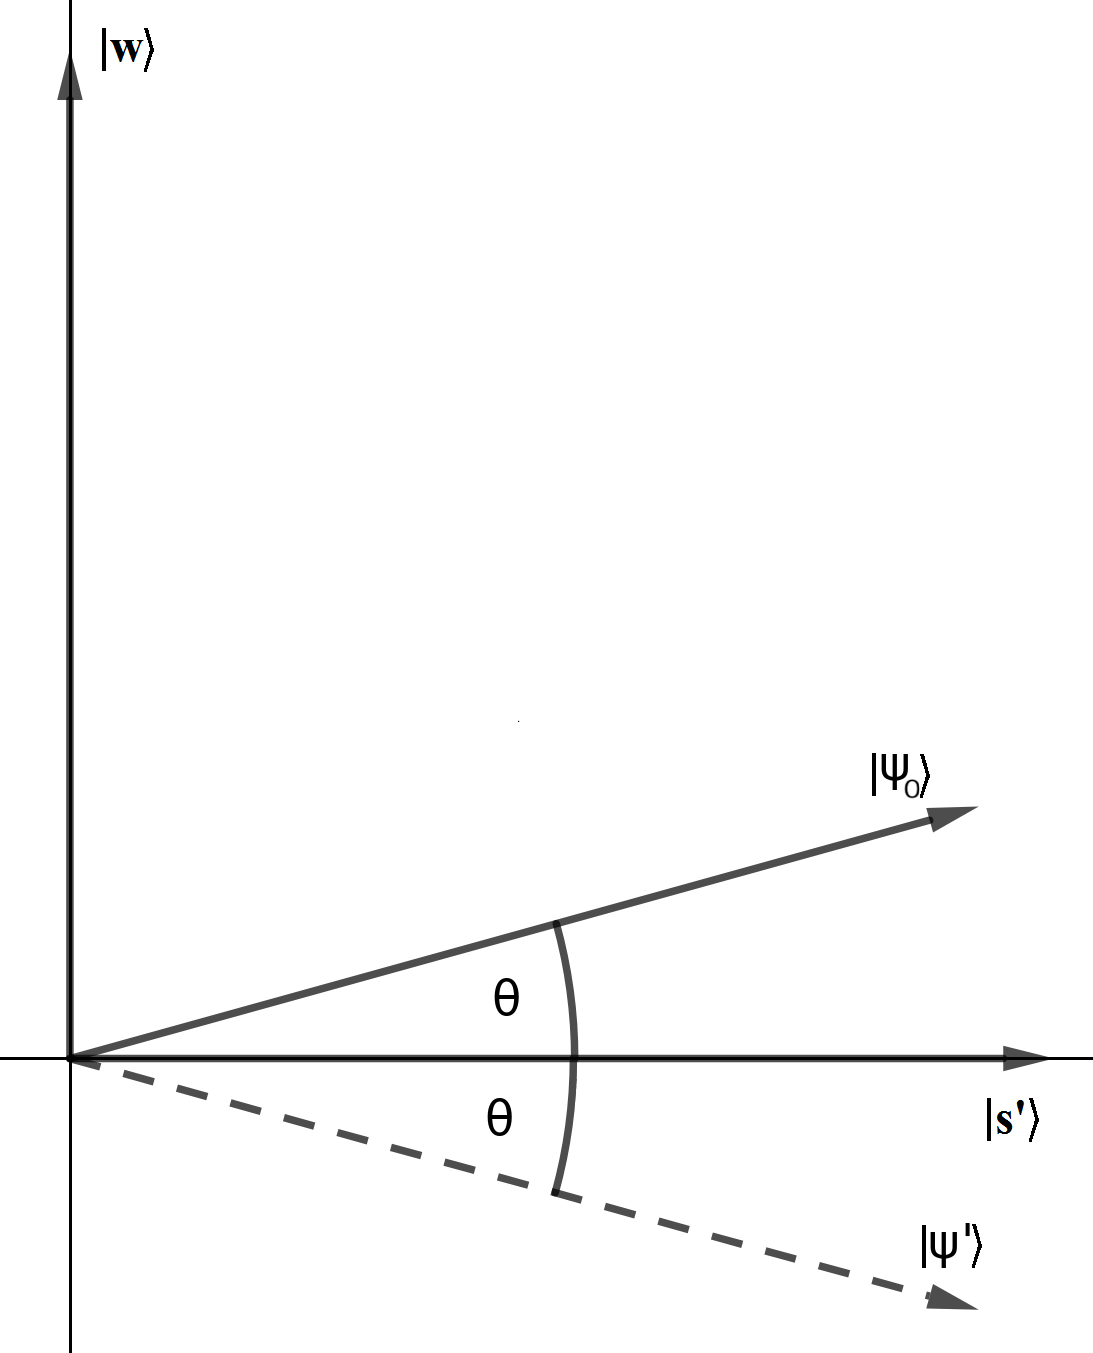
\includegraphics[scale=0.2]{grover_2}
\caption{Action of operator $U_f$ as rotation.}
\end{figure}

The last operator needed in the Grover's algorithm will be denoted as $U_s$. It amplifies factor $c_i$, which are negative and diminishes the positive $c_i$. Action of operator $U_s$ is shown in the bar diagram:

\newpage
\begin{figure}[ht]
\centering
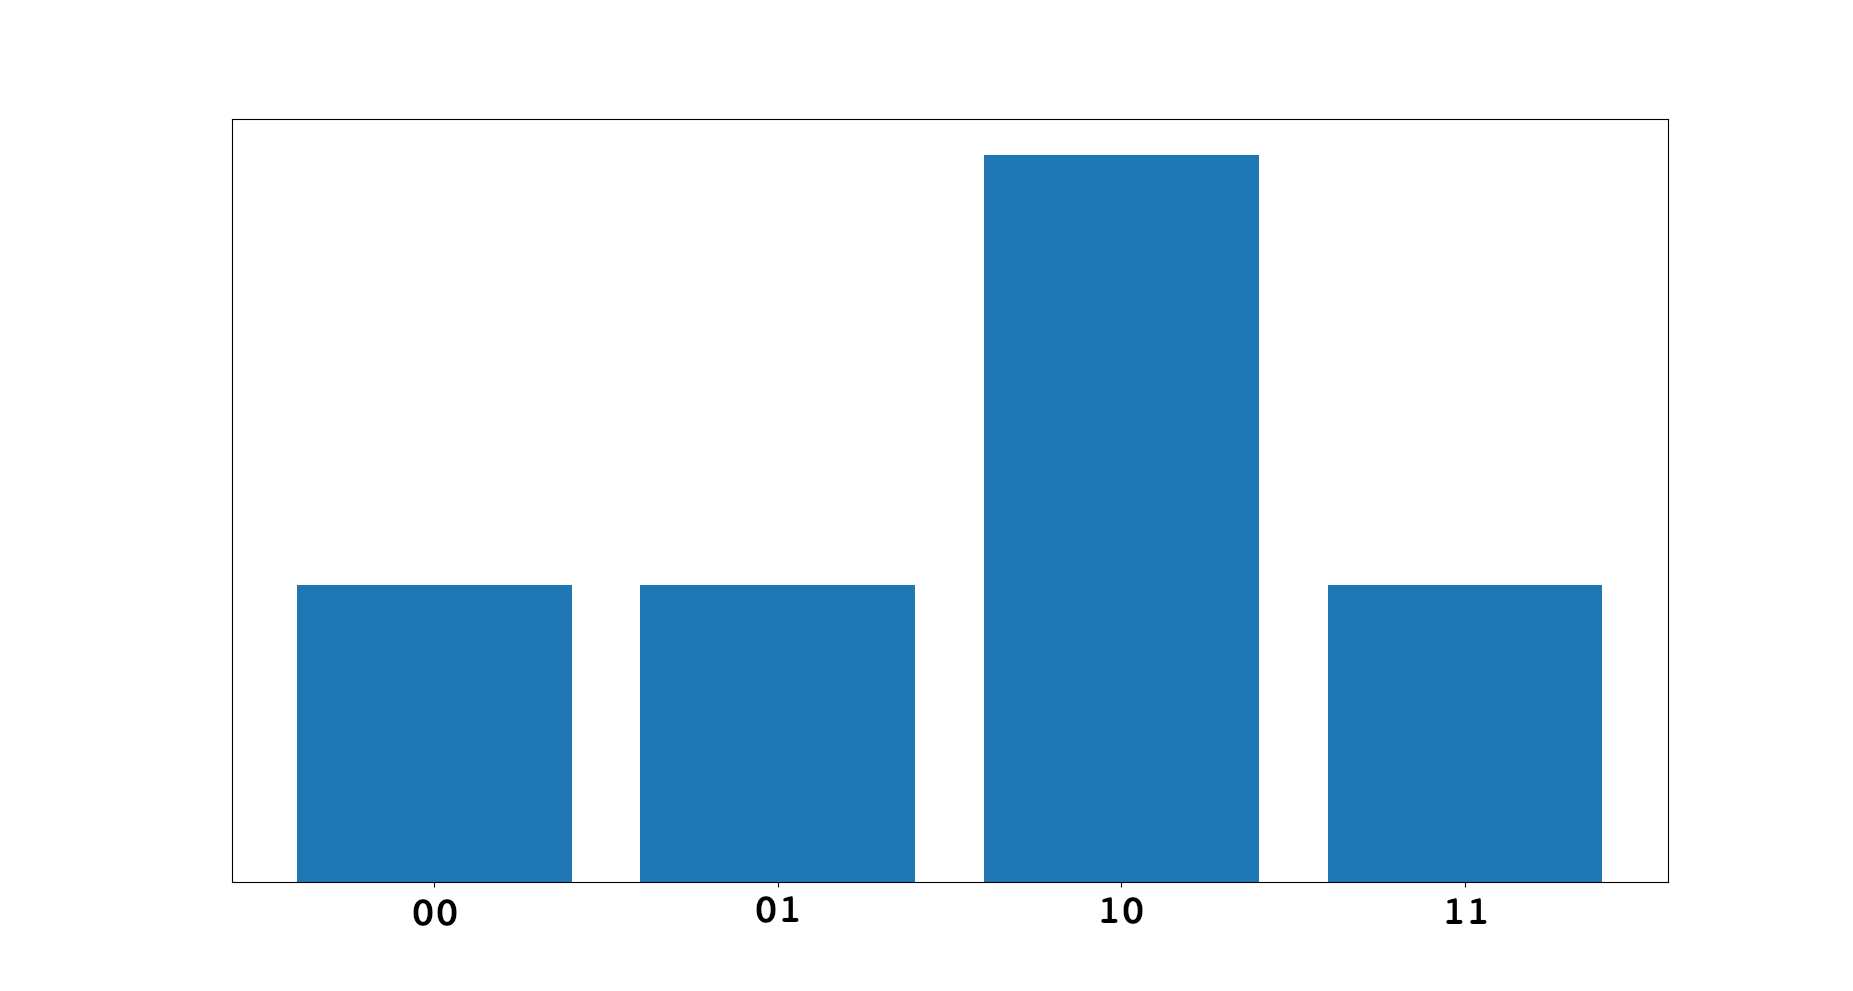
\includegraphics[scale=0.25]{grover_bars_3.png}
\caption{Bar diagram of the vector $U_sU_f|\psi_0\rangle$ (it is not fully correct, which is explained in the below remark).}
\label{grover_bars_3}
\end{figure}

This operator can be also understood as another rotation, but this time it rotates around the average amplitude of all states. It is shown in the picture below:

\begin{figure}[ht]
\centering
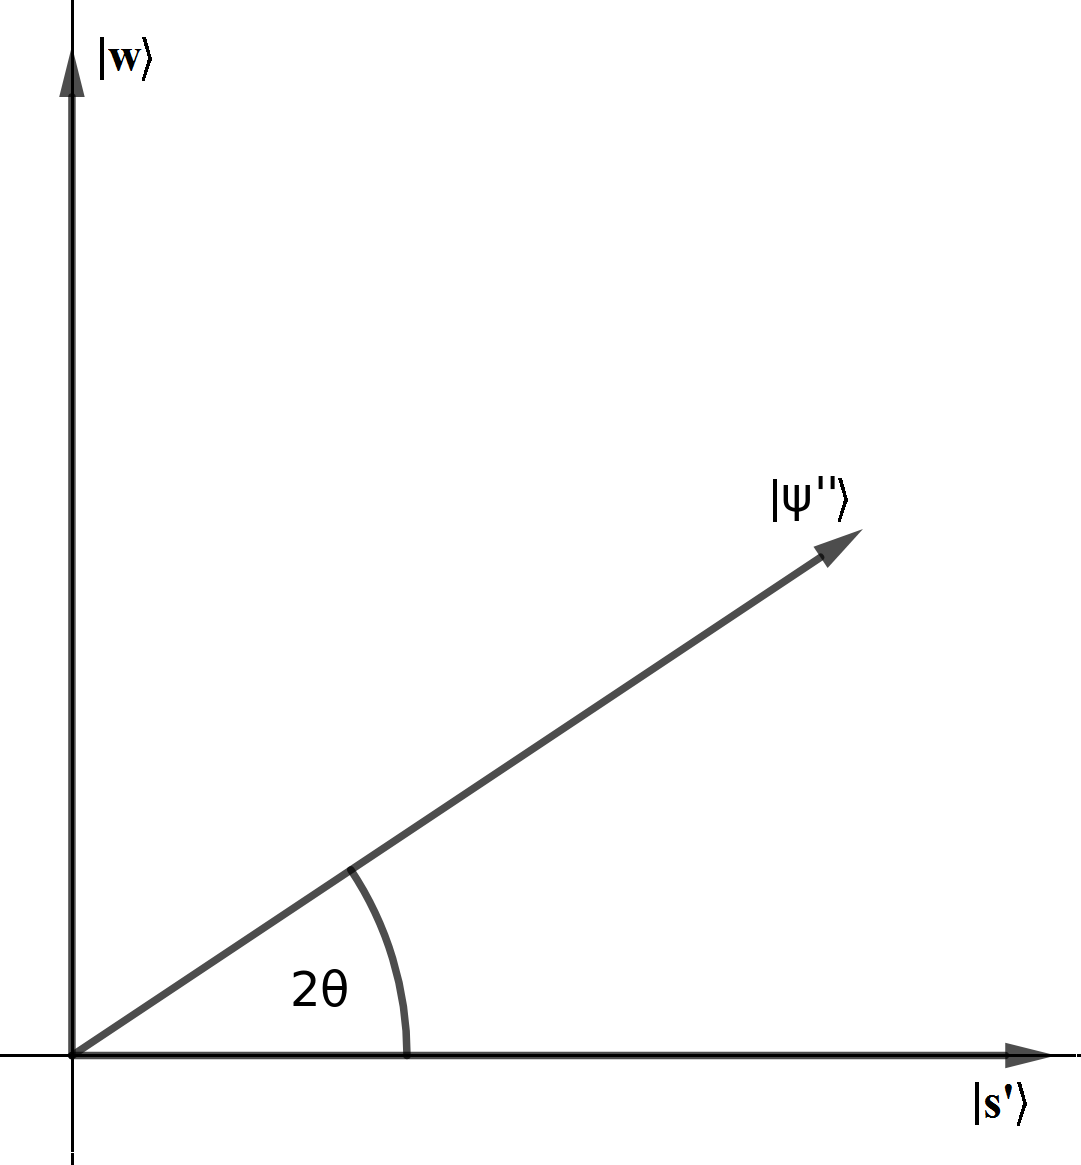
\includegraphics[scale=0.2]{grover_3.png}
\caption{Action of operator $U_s$ as rotation.}
\end{figure}

\begin{remark}
In fact, in our case the average amplitude is equal to $\frac{1}{2}$, so the operator $U_f$ would decrease probabilities $c_0$, $c_1$ and $c_3$ to 0 (because the average amplitude would be exactly in the middle of each of these factors) and increase the $c_2$ to 1 (it cannot be higher, because state vector has to be normalized). The illustration \ref{grover_bars_3} is not fully correct, because factors $c_0$, $c_1$ and $c_2$ should be equal to 0, but it was presented in this way, to give the reader an intuition, of how the $U_s$ operator works.
\end{remark}

Summarizing, Grover's algorithm applies to the initial state operators $U_f$ and $U_s$ as long as the probability of obtaining desired element from database is maximal. In fact, these operations have to applied about $\sqrt{N}$ (where N is the number of elements $N = 2^n$), because using them more than $\sqrt{N}$ times would result in a decrease in probability of obtaining the searched item. This is a great speed-up comparing to the classical algorithms, because the case with uniformly generated calls to a database would result in average cost equal to $\frac{n}{2}$!

The pseudocode of the Grover's algorithm is given below:

\begin{algorithm}[H]
        Initialize the $|\psi_0\rangle$ state (it also can be a result of some other algorithm),\\
        \For{$O(\sqrt{N})$ \  times}{
            \begin{itemize}
                \item apply the $U_f$ operator,
                \item apply the $U_s$ operator,
            \end{itemize}
        }
        measure the resulting state.
 \caption{Pseudocode of the Grover's algorithm}
\end{algorithm}

The implementation of operators $U_f$ and $U_s$ on quantum gates will be presented in the following subsections. At this point we will only point out, that $U_s$ can be obtained by

\[ U_s = 2|s\rangle \langle s| - \mathbb{1},\]

which can be expanded as

\[ U_s = 2 \begin{pmatrix} \frac{1}{\sqrt{N}} \\ \frac{1}{\sqrt{N}} \\ \vdots \\ \frac{1}{\sqrt{N}} \end{pmatrix} \begin{pmatrix} \frac{1}{\sqrt{N}} & \frac{1}{\sqrt{N}} & \hdots & \frac{1}{\sqrt{N}} \end{pmatrix} - \begin{pmatrix} 1 & 0 & \hdots & 0 \\ 0 & 1 & & & \\ \vdots & & \ddots & \\ 0 & & & 1 \end{pmatrix} = \]

\[ 2 \begin{pmatrix} \frac{1}{N} & \frac{1}{N} & \hdots & \frac{1}{N} \\ \frac{1}{N} & \frac{1}{N} & & & \\ \vdots & & \ddots & \\ \frac{1}{N} & & & \frac{1}{N} \end{pmatrix} - \begin{pmatrix} 1 & 0 & \hdots & 0 \\ 0 & 1 & & & \\ \vdots & & \ddots & \\ 0 & & & 1 \end{pmatrix} = \]

\[\begin{pmatrix} \frac{2 - N}{N} & \frac{2}{N} & \hdots & \frac{2}{N} \\ \frac{2}{N} & \frac{2 - N}{N} & & & \\ \vdots & & \ddots & \\ \frac{2}{N} & & & \frac{2 - N}{N} \end{pmatrix}\]

\begin{example}
We will now show the example of searching for a number 2 in our quantum database. We will be using 2 qubits, so we obtain total amount of possible numbers to store equal $N = 2^n = 4$.

Initially, each qubit is in state $|0\rangle$, so the state of the whole system is equal to

\[ |0\rangle \otimes |0\rangle = \begin{pmatrix} 1 \\ 0 \end{pmatrix} \otimes \begin{pmatrix} 1 \\ 0 \end{pmatrix} = \begin{pmatrix} 1 \\ 0 \\ 0 \\ 0 \end{pmatrix}\]

First step is to apply Hadamard gate to each of the qubits. We create $H^{\otimes 2}$ as follows:

\[ H \otimes H = \frac{1}{\sqrt{2}} \begin{pmatrix} 1 & 1 \\ 1 & -1 \end{pmatrix} \otimes \frac{1}{\sqrt{2}} \begin{pmatrix} 1 & 1 \\ 1 & -1 \end{pmatrix} = \frac{1}{2} \begin{pmatrix} 1 & 1 & 1 & 1 \\ 1 & -1 & 1 & -1 \\ 1 & 1 & -1 & -1 \\ 1 & -1 & -1 & 1\end{pmatrix}\]

Now we use the $H^{\otimes 2}$ gate on the $|\psi_0\rangle$ state

\[ |\psi_0\rangle = H^{\otimes 2} |00\rangle = \frac{1}{2} \begin{pmatrix} 1 & 1 & 1 & 1 \\ 1 & -1 & 1 & -1 \\ 1 & 1 & -1 & -1 \\ 1 & -1 & -1 & 1\end{pmatrix} \cdot \begin{pmatrix} 1 \\ 0 \\ 0 \\ 0 \end{pmatrix} = \frac{1}{2} \begin{pmatrix} 1 \\ 1 \\ 1 \\ 1 \end{pmatrix}\]

Each $c_i$ factor is equal to $\frac{1}{2}$, so we obtained the uniform superposition. Now we will use the operator $U_f$. For the purpose of this example we will assume, that we are in possession of a black box performing the action of the $U_f$ operator. It should recognize the state $|10\rangle$, which can be written as

\[ |1\rangle \otimes |0\rangle = \begin{pmatrix} 0 \\ 1 \end{pmatrix} \otimes \begin{pmatrix} 1 \\ 0 \end{pmatrix} = \begin{pmatrix} 0 \\ 0 \\ 1 \\ 0 \end{pmatrix},\]

so it should change the value on the third index in the $|\psi_0\rangle$ vector:

\[ |\psi'\rangle = U_f |\psi_0\rangle = \frac{1}{2}\begin{pmatrix} 1 \\ 1 \\ -1 \\ 1 \end{pmatrix}. \]

We have, that $N = 4$, so the $U_s$ operator is in the form

\[ U_s = \begin{pmatrix} \frac{2 - 4}{4} & \frac{2}{4} & \frac{2}{4} & \frac{2}{4} \\ \\ \frac{2}{4} & \frac{2 - 4}{4} & \frac{2}{4} & \frac{2}{4} \\ \\ \frac{2}{4} & \frac{2}{4} & \frac{2 - 4}{4} & \frac{2}{4} \\ \\ \frac{2}{4} & \frac{2}{4} & \frac{2}{4} & \frac{2 - 4}{4} \end{pmatrix} = \begin{pmatrix} -\frac{1}{2} & \frac{1}{2} & \frac{1}{2} & \frac{1}{2} \\ \\ \frac{1}{2} & -\frac{1}{2} & \frac{1}{2} & \frac{1}{2} \\ \\ \frac{1}{2} & \frac{1}{2} & -\frac{1}{2} & \frac{1}{2} \\ \\ \frac{1}{2} & \frac{1}{2} & \frac{1}{2} & -\frac{1}{2} \end{pmatrix}\]

We apply the $U_s$ operator to the $|\psi'\rangle$ state:

\[ |\psi''\rangle = \begin{pmatrix} -\frac{1}{2} & \frac{1}{2} & \frac{1}{2} & \frac{1}{2} \\ \\ \frac{1}{2} & -\frac{1}{2} & \frac{1}{2} & \frac{1}{2} \\ \\ \frac{1}{2} & \frac{1}{2} & -\frac{1}{2} & \frac{1}{2} \\ \\ \frac{1}{2} & \frac{1}{2} & \frac{1}{2} & -\frac{1}{2} \end{pmatrix} \cdot \frac{1}{2}\begin{pmatrix} 1 \\ 1 \\ -1 \\ 1 \end{pmatrix} =  \frac{1}{4} \begin{pmatrix} -1 & 1 & 1 & 1 \\ 1 & -1 & 1 & 1 \\ 1 & 1 & -1 & 1 \\ 1 & 1 & 1 & -1 \end{pmatrix} \cdot \begin{pmatrix} 1 \\ 1 \\ -1 \\ 1 \end{pmatrix} = \begin{pmatrix} 0 \\ 0 \\ 1 \\ 0 \end{pmatrix}\]

After applying measurement we would obtain state $|10\rangle$ with probability equal to 1. In our example just one iteration was enough to obtain the best possible result.

But let's see what happens, if we apply the whole procedure one more time. We are using $U_f$ on the $|\psi''\rangle$ state and obtain

\[ |\psi'''\rangle = U_f |\psi''\rangle = \begin{pmatrix} 0 \\ 0 \\ -1 \\ 0 \end{pmatrix}. \]

Then, we are using the $U_s$ operator on the $|\psi'''\rangle$ state and get

\[ U_s|\psi'''\rangle = \frac{1}{2}\begin{pmatrix} -1 & 1 & 1 & 1 \\ 1 & -1 & 1 & 1 \\ 1 & 1 & -1 & 1 \\ 1 & 1 & 1 & -1 \end{pmatrix} \cdot \begin{pmatrix} 0 \\ 0 \\ -1 \\ 0 \end{pmatrix} = \begin{pmatrix} -\frac{1}{2} \\ \\ -\frac{1}{2} \\ \\ \frac{1}{2} \\ \\ -\frac{1}{2}  \end{pmatrix}, \]

so the probability, that the system will collapse in any of the possible states is equal to $\frac{1}{4}$. This shows, that using the whole procedure too many times decreases the probability of getting desired element from a quantum database.
\end{example}

\subsection{Implementation of the $U_f$ operator}

In this subsection we will show how to implement on quantum gates a simple operator recognizing a specific number (although, as mentioned before, it is possible to create a function with a wider application). In fact, such an operator can be made out of $C^nZ$ gate with additional \textit{X} gates surrounding the control qubits, which are supposed to be in the $|0\rangle$ state (when considering a register with $n + 1$ qubits).

Based on the above statement we present the quantum circuit recognizing the $|101\rangle$ number:

\[  \scalebox{1.5}{\Qcircuit @C=1em @R=1em {
 & \qw & \ctrl{2} & \qw & \qw \\
 & \gate{X} & \ctrl{1} & \gate{X} & \qw \\
 & \qw & \gate{Z} & \qw & \qw
}} \]

It might be difficult to physically implement the $C^n Z$ gate, so we can decompose this circuit using a borrowed qubit, basing on the knowledge from the second chapter:

\begin{table}[ht]
\centering
\begin{tikzpicture}
\node (a) at (-40,0){
\scalebox{1.3}{\Qcircuit @C=1em @R=1em {
 & \qw & \ctrl{2} & \qw & \qw \\
 & \gate{X} & \ctrl{1} & \gate{X} & \qw \\
 & \qw & \gate{Z} & \qw & \qw
}}
};
\node[yshift=-3.5cm] (b) at (a.south) 
{
\scalebox{1.3}{\Qcircuit @C=1em @R=1em {
 & \lstick{|BO_1\rangle} & \qw & \targ & \ctrl{3} & \targ & \qw & \qw \\
 & & \qw & \ctrl{-1} & \qw & \ctrl{-1} & \qw & \qw \\
 & & \gate{X} & \ctrl{-2} & \qw & \ctrl{-2} & \gate{X} & \qw \\
 & & \qw & \qw & \gate{Z} & \qw & \qw & \qw \\
}}
};
\draw[->,ultra thick](a)--(b);
\end{tikzpicture}
\label{my-label}
\end{table}

Let's try to write this quantum circuit as a matrix. Firstly, we will add the identity gates where it is necessary:

\begin{table}[ht]
\centering
\begin{tikzpicture}
\node (a) at (-40,0){
\scalebox{1.3}{\Qcircuit @C=1em @R=1em {
 & \qw & \ctrl{2} & \qw & \qw \\
 & \gate{X} & \ctrl{1} & \gate{X} & \qw \\
 & \qw & \gate{Z} & \qw & \qw
}}
};
\node[xshift=3.5cm] (b) at (a.east) 
{
\scalebox{1.3}{\Qcircuit @C=1em @R=1em {
 & \gate{I} & \ctrl{2} & \gate{I} & \qw \\
 & \gate{X} & \ctrl{1} & \gate{X} & \qw \\
 & \gate{I} & \gate{Z} & \gate{I} & \qw
}}
};
\draw[->,ultra thick](a)--(b);
\end{tikzpicture}
\label{my-label}
\end{table}

The first layer can be written as

\[ C_1 = I \otimes X \otimes I = \begin{pmatrix} 1 & 0 \\ 0 & 1 \end{pmatrix} \otimes \begin{pmatrix} 0 & 1 \\ 1 & 0 \end{pmatrix} \otimes \begin{pmatrix} 1 & 0 \\ 0 & 1 \end{pmatrix} = \]

\[ \begin{pmatrix} 0 & 1 & 0 & 0 \\ 1 & 0 & 0 & 0 \\ 0 & 0 & 0 & 1 \\ 0 & 0 & 1 & 0 \end{pmatrix} \otimes \begin{pmatrix} 1 & 0 \\ 0 & 1 \end{pmatrix} = \]

\[ \begin{pmatrix}
0 & 0 & 1 & 0 & 0 & 0 & 0 & 0 \\
0 & 0 & 0 & 1 & 0 & 0 & 0 & 0 \\
1 & 0 & 0 & 0 & 0 & 0 & 0 & 0 \\
0 & 1 & 0 & 0 & 0 & 0 & 0 & 0 \\
0 & 0 & 0 & 0 & 0 & 0 & 1 & 0 \\
0 & 0 & 0 & 0 & 0 & 0 & 0 & 1 \\
0 & 0 & 0 & 0 & 1 & 0 & 0 & 0 \\
0 & 0 & 0 & 0 & 0 & 1 & 0 & 0
\end{pmatrix}\]

The second layer consists only of the $C^2Z$ gate, which can be written as

\[ \begin{pmatrix}
1 & 0 & 0 & 0 & 0 & 0 & 0 & 0 \\
0 & 1 & 0 & 0 & 0 & 0 & 0 & 0 \\
0 & 0 & 1 & 0 & 0 & 0 & 0 & 0 \\
0 & 0 & 0 & 1 & 0 & 0 & 0 & 0 \\
0 & 0 & 0 & 0 & 1 & 0 & 0 & 0 \\
0 & 0 & 0 & 0 & 0 & 1 & 0 & 0 \\
0 & 0 & 0 & 0 & 0 & 0 & 1 & 0 \\
0 & 0 & 0 & 0 & 0 & 0 & 0 & -1
\end{pmatrix} \]

The last layer is the same as the first one, so we already have a matrix for it. Now lets multiply all of these matrices to obtain our desired $U_f$ matrix

\[ U_f = C_1 \cdot C^2Z \cdot C_1 = \]

\[ \begin{pmatrix}
0 & 0 & 1 & 0 & 0 & 0 & 0 & 0 \\
0 & 0 & 0 & 1 & 0 & 0 & 0 & 0 \\
1 & 0 & 0 & 0 & 0 & 0 & 0 & 0 \\
0 & 1 & 0 & 0 & 0 & 0 & 0 & 0 \\
0 & 0 & 0 & 0 & 0 & 0 & 1 & 0 \\
0 & 0 & 0 & 0 & 0 & 0 & 0 & 1 \\
0 & 0 & 0 & 0 & 1 & 0 & 0 & 0 \\
0 & 0 & 0 & 0 & 0 & 1 & 0 & 0
\end{pmatrix} \cdot \begin{pmatrix}
1 & 0 & 0 & 0 & 0 & 0 & 0 & 0 \\
0 & 1 & 0 & 0 & 0 & 0 & 0 & 0 \\
0 & 0 & 1 & 0 & 0 & 0 & 0 & 0 \\
0 & 0 & 0 & 1 & 0 & 0 & 0 & 0 \\
0 & 0 & 0 & 0 & 1 & 0 & 0 & 0 \\
0 & 0 & 0 & 0 & 0 & 1 & 0 & 0 \\
0 & 0 & 0 & 0 & 0 & 0 & 1 & 0 \\
0 & 0 & 0 & 0 & 0 & 0 & 0 & -1
\end{pmatrix} \cdot \begin{pmatrix}
0 & 0 & 1 & 0 & 0 & 0 & 0 & 0 \\
0 & 0 & 0 & 1 & 0 & 0 & 0 & 0 \\
1 & 0 & 0 & 0 & 0 & 0 & 0 & 0 \\
0 & 1 & 0 & 0 & 0 & 0 & 0 & 0 \\
0 & 0 & 0 & 0 & 0 & 0 & 1 & 0 \\
0 & 0 & 0 & 0 & 0 & 0 & 0 & 1 \\
0 & 0 & 0 & 0 & 1 & 0 & 0 & 0 \\
0 & 0 & 0 & 0 & 0 & 1 & 0 & 0
\end{pmatrix} = \]

\[
\begin{pmatrix}
1 & 0 & 0 & 0 & 0 & 0 & 0 & 0 \\
0 & 1 & 0 & 0 & 0 & 0 & 0 & 0 \\
0 & 0 & 1 & 0 & 0 & 0 & 0 & 0 \\
0 & 0 & 0 & 1 & 0 & 0 & 0 & 0 \\
0 & 0 & 0 & 0 & 1 & 0 & 0 & 0 \\
0 & 0 & 0 & 0 & 0 & -1 & 0 & 0 \\
0 & 0 & 0 & 0 & 0 & 0 & 1 & 0 \\
0 & 0 & 0 & 0 & 0 & 0 & 0 & 1
\end{pmatrix}
\]

Let's check, if this matrix works as we want it to. It should recognize the $|101\rangle$ state, which can be written as

\[ |101\rangle = \begin{pmatrix} 0 \\ 1 \end{pmatrix} \otimes \begin{pmatrix} 1 \\ 0 \end{pmatrix} \otimes \begin{pmatrix} 0 \\ 1 \end{pmatrix} = \begin{pmatrix} 0 \\ 0 \\ 0 \\ 0 \\ 0 \\ 1 \\ 0 \\ 0 \end{pmatrix}\]

We can see, that our matrix in fact flips the amplitude of probability of such a vector

\[ U_f |101\rangle = \begin{pmatrix}
1 & 0 & 0 & 0 & 0 & 0 & 0 & 0 \\
0 & 1 & 0 & 0 & 0 & 0 & 0 & 0 \\
0 & 0 & 1 & 0 & 0 & 0 & 0 & 0 \\
0 & 0 & 0 & 1 & 0 & 0 & 0 & 0 \\
0 & 0 & 0 & 0 & 1 & 0 & 0 & 0 \\
0 & 0 & 0 & 0 & 0 & -1 & 0 & 0 \\
0 & 0 & 0 & 0 & 0 & 0 & 1 & 0 \\
0 & 0 & 0 & 0 & 0 & 0 & 0 & 1
\end{pmatrix} \cdot \begin{pmatrix} 0 \\ 0 \\ 0 \\ 0 \\ 0 \\ 1 \\ 0 \\ 0 \end{pmatrix} = \begin{pmatrix} 0 \\ 0 \\ 0 \\ 0 \\ 0 \\ -1 \\ 0 \\ 0 \end{pmatrix},\]

which proves, that the whole structure is correct.

\begin{remark}
If, for some reason, we were unable to use the \textit{Z} gate, it could be replaced by \textit{HXH} gates:

\[ HXH = \frac{1}{\sqrt{2}} \begin{pmatrix} 1 & 1 \\ 1 & -1 \end{pmatrix} \cdot \frac{1}{\sqrt{2}}\begin{pmatrix} 0 & 1 \\ 1 & 0 \end{pmatrix} \cdot \begin{pmatrix} 1 & 1 \\ 1 & -1 \end{pmatrix} = \begin{pmatrix} 1 & 0 \\ 0 & -1 \end{pmatrix} = Z.\]

The same works in the other way - we can replace the \textit{X} gate with \textit{HZH} gates:

\[ HZH = \frac{1}{\sqrt{2}} \begin{pmatrix} 1 & 1 \\ 1 & -1 \end{pmatrix} \cdot \begin{pmatrix} 1 & 0 \\ 0 & -1 \end{pmatrix} \cdot \frac{1}{\sqrt{2}} \begin{pmatrix} 1 & 1 \\ 1 & -1 \end{pmatrix} = \begin{pmatrix} 0 & 1 \\ 1 & 0 \end{pmatrix} = X.\]

\end{remark}

\subsection{Implementation of the $-U_s$ operator}

In this subsection we will show how to implement the $-U_s$ operator. Its action will be the same as the $U_s$ operator, with the only difference being a "\textit{-}" sign next to probability amplitudes, which does not change the results of measurement, because we are always obtaining state with the probability equal to square of the amplitude.

The $-U_s$ operator can be created in the following way:

\[ -U_s = H^{\otimes n} X^{\otimes n} C^{n-1}Z X^{\otimes n} H^{\otimes n}.\]

An example quantum circuit with three qubits is given below

\[ \scalebox{1.5}{\Qcircuit @C=1em @R=.7em {
& \multigate{2}{H^{\otimes 3}} & \multigate{2}{X^{\otimes 3}} & \ctrl{2} & \multigate{2}{X^{\otimes 3}} & \multigate{2}{H^{\otimes 3}} & \qw \\
& \ghost{H^{\otimes 3}} & \ghost{X^{\otimes 3}} & \ctrl{1} & \ghost{X^{\otimes 3}} & \ghost{H^{\otimes 3}} & \qw \\
& \ghost{H^{\otimes 3}} & \ghost{X^{\otimes 3}} & \gate{Z} & \ghost{X^{\otimes 3}} & \ghost{H^{\otimes 3}} & \qw
}} \]

It can be decomposed using one borrowed qubit:

\[ \scalebox{1.5}{\Qcircuit @C=1em @R=.7em {
& \lstick{|BO_1\rangle} & \qw & \qw & \targ & \ctrl{3} & \targ & \qw & \qw & \qw \\
& & \multigate{2}{H^{\otimes 3}} & \multigate{2}{X^{\otimes 3}} & \ctrl{-1} & \qw & \ctrl{-1} & \multigate{2}{X^{\otimes 3}} & \multigate{2}{H^{\otimes 3}} & \qw \\
& & \ghost{H^{\otimes 3}} & \ghost{X^{\otimes 3}} & \ctrl{-2} & \qw & \ctrl{-2} & \ghost{X^{\otimes 3}} & \ghost{H^{\otimes 3}} & \qw \\
& & \ghost{H^{\otimes 3}} & \ghost{X^{\otimes 3}} & \qw & \gate{Z} & \qw & \ghost{X^{\otimes 3}} & \ghost{H^{\otimes 3}} & \qw
}} \]

Let's write all layers of this circuit in the matrix form:

\[ H^{\otimes 3} = \frac{1}{2\sqrt{2}}\begin{pmatrix}
1 & 1 & 1 & 1 & 1 & 1 & 1 & 1 \\
1 & -1 & 1 & -1 & 1 & -1 & 1 & -1 \\
1 & 1 & -1 & -1 & 1 & 1 & -1 & -1 \\
1 & -1 & -1 & 1 & 1 & -1 & -1 & 1 \\
1 & 1 & 1 & 1 & -1 & -1 & -1 & -1 \\
1 & -1 & 1 & -1 & -1 & 1 & -1 & 1 \\
1 & 1 & -1 & -1 & -1 & -1 & 1 & 1 \\
1 & -1 & -1 & 1 & -1 & 1 & 1 & -1 
\end{pmatrix}\]

\[ X^{\otimes 3} = \begin{pmatrix}
0 & 0 & 0 & 0 & 0 & 0 & 0 & 1 \\
0 & 0 & 0 & 0 & 0 & 0 & 1 & 0 \\
0 & 0 & 0 & 0 & 0 & 1 & 0 & 0 \\
0 & 0 & 0 & 0 & 1 & 0 & 0 & 0 \\
0 & 0 & 0 & 1 & 0 & 0 & 0 & 0 \\
0 & 0 & 1 & 0 & 0 & 0 & 0 & 0 \\
0 & 1 & 0 & 0 & 0 & 0 & 0 & 0 \\
1 & 0 & 0 & 0 & 0 & 0 & 0 & 0
\end{pmatrix}\]

\[ C^2 Z = \begin{pmatrix}
1 & 0 & 0 & 0 & 0 & 0 & 0 & 0 \\
0 & 1 & 0 & 0 & 0 & 0 & 0 & 0 \\
0 & 0 & 1 & 0 & 0 & 0 & 0 & 0 \\
0 & 0 & 0 & 1 & 0 & 0 & 0 & 0 \\
0 & 0 & 0 & 0 & 1 & 0 & 0 & 0 \\
0 & 0 & 0 & 0 & 0 & 1 & 0 & 0 \\
0 & 0 & 0 & 0 & 0 & 0 & 1 & 0 \\
0 & 0 & 0 & 0 & 0 & 0 & 0 & -1
\end{pmatrix} \]

All of these combined give us the final matrix

\[ -U_s = H^{\otimes n} X^{\otimes n} C^{n-1}Z X^{\otimes n} H^{\otimes n} = \frac{1}{4}\begin{pmatrix}
3 & -1 & -1 & -1 & -1 & -1 & -1 & -1 \\
-1 & 3 & -1 & -1 & -1 & -1 & -1 & -1 \\
-1 & -1 & 3 & -1 & -1 & -1 & -1 & -1 \\
-1 & -1 & -1 & 3 & -1 & -1 & -1 & -1 \\
-1 & -1 & -1 & -1 & 3 & -1 & -1 & -1 \\
-1 & -1 & -1 & -1 & -1 & 3 & -1 & -1 \\
-1 & -1 & -1 & -1 & -1 & -1 & 3 & -1 \\
-1 & -1 & -1 & -1 & -1 & -1 & -1 & 3 \\
\end{pmatrix} \]

Let's see this matrix in action. By applying $H^{\otimes 3}$ gate to the initial $|000\rangle$ state we are getting the uniform superposition:

\[ H^{\otimes 3} |000\rangle = \frac{1}{2\sqrt{2}}\begin{pmatrix}
1 \\ 1 \\ 1 \\ 1 \\ 1 \\ 1 \\ 1 \\ 1
\end{pmatrix}.\]

After applying the $U_f$ operator we are obtaining the state

\[ \frac{1}{2\sqrt{2}}\begin{pmatrix}
1 \\ 1 \\ 1 \\ 1 \\ 1 \\ -1 \\ 1 \\ 1
\end{pmatrix}.\]

Finally, using the $-U_s$ matrix gives us

\[ -U_s \frac{1}{2\sqrt{2}}\begin{pmatrix} 1 \\ 1 \\ 1 \\ 1 \\ 1 \\ -1 \\ 1 \\ 1 \end{pmatrix} = \frac{1}{4\sqrt{2}}\begin{pmatrix}
-1 \\ -1 \\ -1 \\ -1 \\ -1 \\ -5 \\ -1 \\ -1 \end{pmatrix}.\]

If we apply the $U_f$ and $-U_s$ operators one more time we will obtain the best possible outcome for the case with three qubits:

\[ -U_s U_f \frac{1}{4\sqrt{2}}\begin{pmatrix} -1 \\ -1 \\ -1 \\ -1 \\ -1 \\ -5 \\ -1 \\ -1 \end{pmatrix} = 
\frac{1}{8\sqrt{2}} \begin{pmatrix}
-1 \\ -1 \\ -1 \\ -1 \\ -1 \\ 11 \\ -1 \\ -1 \end{pmatrix}\]

\subsection{Final version of the Grover's algorithm}

We have shown all steps needed to construct the Grover's algorithm. Its pseudocode is written below

\begin{algorithm}[H]
    Apply the $H^{\otimes n}$ gate to the initial $|00...0\rangle$ state to obtain uniform superposition, \\
    generate a binary representation of searched number, \\
    \For{$O(\sqrt{N})$ \  times}{
        \begin{itemize}
            \item add the $C^{n-1}Z$ gate and surround control qubits, which are supposed to be equal to 0, with \textit{X} gates,
            \item add the $H^{\otimes n}$ gate,
            \item add the $X^{\otimes n}$ gate,
            \item add the $C^{n-1}Z$ gate,
            \item add the $X^{\otimes n}$ gate,
            \item add the $H^{\otimes n}$ gate,
        \end{itemize}
    }
    measure the resulting state.
 \caption{Pseudocode of the Grover's algorithm for a uniform superposition}
\end{algorithm}

Full code of the program using \textit{qiskit} is presented in the appendix \ref{appendixA}. An example quantum circuit, compatible with the above pseudocode, is given below (for $n = 3$, $U_f$ finding the number 0 and only one iteration of the algorithm):

\[  \scalebox{1.5}{\Qcircuit @C=1em @R=1em {
    & \gate{H} & \gate{X} & \ctrl{2} & \gate{X} & \gate{H} & \gate{X} & \ctrl{2} & \gate{X} & \gate{H} & \qw \\
    & \gate{H} & \gate{X} & \ctrl{1} & \gate{X} & \gate{H} & \gate{X} & \ctrl{1} & \gate{X} & \gate{H} & \qw \\
    & \gate{H} & \gate{X} & \gate{Z} & \gate{X} & \gate{H} & \gate{X} & \gate{Z} & \gate{X} & \gate{H} & \qw \gategroup{1}{3}{3}{5}{.7em}{--} \gategroup{1}{6}{3}{10}{.7em}{--}
}} \]

Groups of gates (surrounded with dashed lines) create the $U_f$ and $-U_s$ operators accordingly. As mentioned earlier, it might be hard to physically implement the $C^n Z$ gate, but we can use one borrowed qubit to modify the above circuit:

\[  \scalebox{1.5}{\Qcircuit @C=1em @R=1em {
    & \qw & \qw & \targ & \ctrl{3} & \targ & \qw & \qw & \qw & \targ & \ctrl{3} & \targ & \qw & \qw & \qw \\
    & \gate{H} & \gate{X} & \ctrl{-1} & \qw & \ctrl{-1} & \gate{X} & \gate{H} & \gate{X} & \ctrl{-1} & \qw & \ctrl{-1} & \gate{X} & \gate{H} & \qw \\
    & \gate{H} & \gate{X} & \ctrl{-2} & \qw & \ctrl{-2} & \gate{X} & \gate{H} & \gate{X} & \ctrl{-2} & \qw & \ctrl{-2} & \gate{X} & \gate{H} & \qw \\
    & \gate{H} & \gate{X} & \qw & \gate{Z} & \qw & \gate{X} & \gate{H} & \gate{X} & \qw & \gate{Z} & \qw & \gate{X} & \gate{H} & \qw \gategroup{1}{3}{4}{7}{.7em}{--} \gategroup{1}{8}{4}{14}{.7em}{--}
}} \]

\[\]

According to the \ref{grover_general}, the above version of Grover's algorithm would work for any initial state (not an uniform superposition), being e.g. result of some other algorithm. Moreover, it is possible to implement quantum algorithm finding minimum in a quantum database (\ref{grover_minimum}). These properties can give a massive speedup in finding solutions of \textit{NP} problems. Let's say, we are trying to find solution to a traveling salesman problem. We could insert lengths of all of the possible routes in a quantum database and use Grover's algorithm, to find the minimum. This leads us to conclusion, that Grover's algorithm can find solutions to \textit{NP} problems in $O(\sqrt{n}$ time (assuming, that we can efficiently create initial quantum state)!

Experimental results for Grover's algorithm are given in the appendix \ref{appendixB}.

\newpage
\section{Algorithms based on the quantum Fourier transform}

We will begin this section by introducing the quantum Fourier transform. We will tell about differences, when comparing it to the classical Fourier transform and show, how it can be implemented on quantum gates. Further, we will gradually present three algorithms basing on this structure: phase estimation, order finding and Shor's factoring algorithms. given these algorithms as a template we will tell about a whole class of algorithms based on quantum Fourier transform. Finally, we will show in detail how Shor's factoring algorithm can be implemented on a quantum computer and present some experimental results.

\subsection{Quantum Fourier transform}

Classical Fourier transform can be understood as a change of basis (its rotation), in which a vector is represented. In this work we will only consider a discrete case of this operation. Mentioned vector can be written as a sequence of complex numbers ${x_i} = (x_1, x_2, ..., x_N)$. \textbf{Discrete Fourier transform} (denoted also as \textbf{DFT}) changes each of vector's components into the new sequence ${y_i} = (y_1, y_2, ..., y_N)$ according to the below formula:

\[ y_k = \frac{1}{\sqrt{N}}\sum_{j = 0}^{N - 1} x_j \cdot e^{-\frac{2 \pi i}{N}jk} = \frac{1}{\sqrt{N}}\sum_{j = 0}^{N - 1} x_j \cdot \bigg[cos\bigg(\frac{2 \pi jk}{N} \bigg) - i \cdot sin\bigg(\frac{2 \pi jk}{N}\bigg)\bigg],\]

where the last transition is based on Euler's formula.

\begin{remark}
Vectors $b_k = (\frac{1}{\sqrt{N}} e^{\frac{2 \pi i}{N} jk} | j = 0, 1, ..., N - 1)^T$ form an orthonormal basis:

\[ \langle b_k | b_{k'} \rangle = \sum_{j = 0}^{N - 1} \bigg(\frac{1}{\sqrt{N}} e^{\frac{2 \pi i}{N}jk}\bigg) \cdot \bigg(\frac{1}{\sqrt{N}} e^{-\frac{2 \pi i}{N}jk'}\bigg) =  \frac{1}{N} \sum_{j = 0}^{N - 1} e^{\frac{2 \pi i}{N} (k - k')j}\]

Now we will consider two cases of the above equation. First case, when $k = k'$ gives us the following result
\[ \frac{1}{N} \sum_{j = 0}^{N - 1} e^{\frac{2 \pi i}{N} 0 \cdot j} = \frac{1}{N} \sum_{j = 0}^{N - 1} 1 = \frac{1}{N} \cdot N = 1. \]

In the other case, when $k \neq k'$ lets denote the result of subtraction $k - k'$ by \textit{t} (so \textit{t} is an integer). Using the formula for the sum of a geometric series we obtain 

\[\frac{1}{N} \sum_{j = 0}^{N - 1} e^{\frac{2 \pi i}{N} t j} = \frac{1 - e^{\frac{2t \pi i}{N}\cdot N}}{1 - e^{\frac{2t \pi i}{N}}} = \frac{1 - e^{2t \pi i}}{1 - e^{\frac{2t \pi i}{N}}}.\]

From the Euler's formula we know, that $e^{2\pi i} = 1$:

\begin{figure}[ht]
\centering
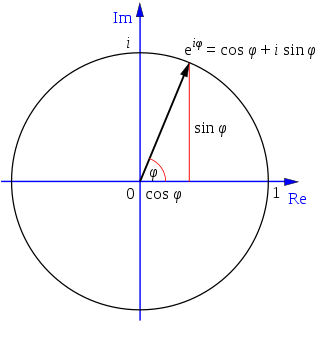
\includegraphics[scale=0.4]{eulers_formula}
\caption{Interpretation of the Euler's formula.}
\end{figure}

\newpage
An integer \textit{t} in the exponent does not change the final result (it can be understood as making many circles around the axes intersection instead of just one). This gives us, that

\[\frac{1 - e^{2t \pi i}}{1 - e^{\frac{2t \pi i}{N}}} = \frac{1 - 1}{1 - e^{\frac{2t \pi i}{N}}} = 0.\]

When we combine the above two cases we see, that the equation from which we started can be written as

\[ \langle b_k | b_{k'} \rangle = \frac{1}{N} \sum_{j = 0}^{N - 1} e^{\frac{2 \pi i}{N} (k - k')j} = \frac{1}{N} \cdot N \cdot \delta_{kk'} = \delta_{kk'}, \]

which proves, that basis vectors $\{b_k\}$ create an orthonormal basis. At the same time we have shown, that discrete Fourier transform (with the $\frac{1}{\sqrt{N}}$ factor) is an \textbf{unitary operation}. Without the $\frac{1}{\sqrt{N}}$ factor this operation would not be unitary.
\end{remark}

The \textbf{quantum Fourier transform} (denoted also as \textbf{QFT}) is an extension of the discrete Fourier transform. It takes into account only vectors of length $N = 2^n$, where \textit{n} is the number of qubits, which we will be using. Qubits create workspace for this operation and, as we stated in the first chapter, when we are considering a compound physical system made of smaller ones, we are using tensor product to describe its behavior. This let's us deduce, that adding a new qubit to the workspace doubles its size. At the same time we are not losing the possibility to transform vectors with odd number of components. We can fill the "missing spaces" with zeroes and use the QFT.

QFT is changing the basis $\{|j\rangle \} = \{ |0\rangle, |1\rangle, ..., |N - 1\rangle \}$ into the new one, similarly to the DFT:

\[ |j\rangle \xrightarrow{\text{QFT}} \frac{1}{\sqrt{N}} \sum_{k = 0}^{N - 1} e^{\frac{2 \pi i}{N} jk} |k\rangle.\]

Other way to write the action of the QFT is given below:

\[ \sum_{j = 0}^{N - 1}x_j |j\rangle \xrightarrow{\text{QFT}} \sum_{k = 0}^{N - 1} y_k |k\rangle,\]

where

\[ y_k = \frac{1}{\sqrt{N}} \sum_{j = 0}^{N - 1} e^{\frac{2 \pi i}{N}jk} x_j.\]

\subsection{Product representation of the quantum Fourier transform}

Before going to the implementation, let's introduce some notation and facts, which will be necessary in this process:

\begin{enumerate}
    \item $N = 2^n$, so the basis consists of states $|0\rangle, |1\rangle, ..., |2^n - 1\rangle$,
    \item binary representation of a number \textit{j} will be denoted as $j = j_1 j_2 ... j_n$, which means
    \[ j = j_1 2^{n - 1} + j_2 2^{n - 2} + ... + j_{n - 1} 2 ^1 + j_n 2^0,\]
    \item notation $0.j_l j_{l+1} ... j_m$ represents $\frac{j_l}{2^1} + \frac{j_{l+1}}{2^2} + ... + \frac{j_{m - 1}}{2^{m - l}} + \frac{j_m}{2^{m - l + 1}}$.
\end{enumerate}

Now we will derive to the result of the QFT acting on given state. This resulting representation will allow us to create a proper quantum circuit. According to the definition, the QFT acting on state $|j\rangle$ can be written as

\[ QFT\ |j\rangle = QFT\ |j_1j_2...j_n\rangle = \frac{1}{2^{\frac{n}{2}}} \sum_{k = 0}^{2^n - 1} e^{\frac{2 \pi ijk}{2^n}} |k\rangle = \]
\[ \frac{1}{2^{\frac{n}{2}}} \sum_{k = 0}^{2^n - 1} e^{\frac{2 \pi ij}{2^n} \sum_{l = 1}^{n}k_l 2^{n - l}} |k_1 k_2 ... k_n\rangle = \]
\[ \frac{1}{2^{\frac{n}{2}}} \sum_{k = 0}^{2^n - 1} e^{2 \pi ij \sum_{l = 1}^{n}k_l 2^{-l}} |k_1 k_2 ... k_n\rangle. \]

Above we replaced $|j\rangle$ and $|k\rangle$ with their binary representations $|j_1j_2...j_n\rangle$ and $|k_1k_2...k_n\rangle$ respectively.

Now we will try to replace the sum $\sum_{k = 0}^{2^n - 1}$ with some other construct. It is important to notice, that in this sum we are going over all of the numbers $0, 1, 2, ..., 2^n - 1$. These numbers can be written in binary form using always \textit{n} bits. Therefore, going through all of these numbers is equivalent to using all of the possible combinations of \textit{n} bits, which can be written as $\sum_{k_1 = 0}^{1}\sum_{k_2 = 0}^{1} ... \sum_{k_n = 0}^{1}$. Finally

\[ \sum_{k = 0}^{2^n - 1} = \sum_{k_1 = 0}^{1} \sum_{k_2 = 0}^{1} ... \sum_{k_n = 0}^{1}.\]

We will use this fact to further decompose considered equation:

\[ \frac{1}{2^{\frac{n}{2}}} \sum_{k = 0}^{2^n - 1} e^{2 \pi ij \sum_{l = 1}^{n}k_l 2^{-l}} |k_1 k_2 ... k_n\rangle = \]
\[ \frac{1}{2^{\frac{n}{2}}} \sum_{k_1 = 0}^{1}\sum_{k_2 = 0}^{1} ... \sum_{k_n = 0}^{1} e^{2 \pi ij \sum_{l = 1}^{n}k_l 2^{-l}} |k_1 k_2 ... k_n\rangle = \]
\[ \frac{1}{2^{\frac{n}{2}}} \sum_{k_1 = 0}^{1}\sum_{k_2 = 0}^{1} ... \sum_{k_n = 0}^{1} e^{2 \pi ij k_1 2^{-1}} \cdot e^{2 \pi ij k_2 2^{-2}} \cdot ... \cdot e^{2 \pi ij k_n 2^{-n}} |k_1 k_2 ... k_n\rangle = \]
\[ \frac{1}{2^{\frac{n}{2}}} \sum_{k_1 = 0}^{1}\sum_{k_2 = 0}^{1} ... \sum_{k_n = 0}^{1} \bigotimes_{l = 1}^{n} e^{2 \pi ij k_l 2^{-l}}|k_l\rangle = \]
\[ \frac{1}{2^{\frac{n}{2}}} \bigotimes_{l=1}^{n} \bigg[ \sum_{k_l = 0}^{1} e^{2 \pi ij k_l 2^{-l}}|k_l\rangle \bigg] = \]
\[ \frac{1}{2^{\frac{n}{2}}} \bigotimes_{l=1}^{n} \bigg[ |0\rangle + e^{2 \pi ij 2^{-l}}|1\rangle \bigg] = \]
\[ \frac{1}{2^{\frac{n}{2}}} \bigotimes_{l=1}^{n} \bigg[ |0\rangle + e^{2 \pi i 2^{-l} \sum_{k = 1}^{n}j_k 2^{n - k}}|1\rangle \bigg] \]

In the last step we just replaced \textit{j} in the exponent by its binary representation. Let's look closer at this exponent. There is a factor $2^{-l}\sum_{k = 1}^{n} j_k 2^{n - k}$, which can be rewritten as

\[ 2^{-l}\sum_{k = 1}^{n} j_k 2^{n - k} = 2^{-l} \bigg( j_1 2^{n - 1} + j_2 2^{n - 2} + ... + j_n 2^0 \bigg) = j_n 2^{-l} + j_{n-1} 2^{-l + 1} + ... + j_1 2^{-l + n - 1}.\]

We also used the tensor product $\bigotimes$ with index \textit{l} going through numbers 1, 2, ..., n. \textit{l} will be at most equal to \textit{n}, so the number $j_n 2^{-l} + j_{n-1} 2^{-l + 1} + ... + j_1 2^{-l + n - 1}$ can be broken down into its integer and fractional parts. For example, for $l = 1$ we obtain

\[ j_{n} 2^{-1} + j_{n-1} 2^{0} + ... + j_{1} 2^{n-2} = 0.j_n + j - 2^{n - 1}, \]

and for $l = 2$ we get

\[ j_{n} 2^{-2} + j_{n-1} 2^{-1} + j_{n-2} 2^{0} + ... + j_{1} 2^{n-3} = 0.j_{n-1} j_n + j - 2^{n - 1} - 2^{n - 2}, \]

where \textit{j} is initial number and $j_i$ are its binary components. Using induction, we can write the final correlation

\[ 2^{-l}\sum_{k = 1}^{n} j_k 2^{n - k} = 0.j_l j_{l+1} ... j_n + \bigg(j - \sum_{i = 0}^{l} j_i 2^{n - 1 - i} \bigg).\]

It is extremely important to notice, for the purpose of further deduction, that part $\bigg(j - \sum_{i = 0}^{l} j_i 2^{n - 1 - i} \bigg)$ \textbf{is an integer}. Because of this we will replace it with symbol \textit{t}, so the upper equation can be rewritten in the form:

\[ 2^{-l}\sum_{k = 1}^{n} j_k 2^{n - k} = 0.j_l j_{l+1} ... j_n + t.\]

Now, let's come back to the whole exponential function, from which we started the above deduction. Having the last statement, we can write, that

\[ e^{2 \pi ij 2^{-l}} = e^{2 \pi i 2^{-l} \sum_{k=1}^{n} j_n 2^{n - k}} = \]
\[ e^{2 \pi i [0.j_l...j_n + (j - \sum_{i = 0}^{l}j_i 2^{n - 1 - i})]} = \]
\[ e^{2 \pi i [0.j_l...j_n + t]} = e^{2 \pi i 0.j_l...j_n} \cdot e^{2 \pi i t}. \]

We have stated, that \textit{t} is an integer. From the Euler's formula we know, that $e^{2 \pi i} = 1$, so number $e^{2 \pi i t}$ will be also equal to 1 (as before, we can interpret this as making many circles around the intersection of axes). Finally we have

\[ e^{2 \pi i j 2^{-l}} = e ^{2 \pi i 0.j_l ... j_n}.\]

\begin{remark}
In the above process we implicitly used the equivalence of usage of different notation. We will show what we mean by this by giving an example. Let's see, what happens with binary representation of number \textit{j} for consecutive values of \textit{l} (we have to remember, that we can ommit the integer part of a number in this reasoning):
\begin{itemize}
    \item l = 1
    \[ j_1 j_2 ... j_n \rightarrow j_1 j_2 ... j_{n-1}.j_n \rightarrow 0.j_n \equiv 0.j_{l'},\  where\ l' = n,\]
    \item l = 2
    \[ j_1 j_2 ... j_n \rightarrow 0.j_{n-1}j_n \equiv 0.j_{l'}j_n,\  where\ l' = n - 1,\]
    $\vdots$ 
    \item l = n - 1
    \[ j_1 j_2 ... j_n \rightarrow 0.j_2 j_3 ... j_n \equiv 0.j_{l'}...j_n,\  where\ l' = 2,\]
    \item l = n
    \[ j_1 j_2 ... j_n \rightarrow 0.j_1 j_2 ... j_n \equiv 0.j_{l'}... j_n,\  where\ l' = 1,\]
\end{itemize}

so we can see, that while considering the final result, which we want to achieve, indices \textit{l} and \textit{l'} can be thought of as equivalent (we only have to reverse the order).
\end{remark}

Using the last received property we can rewrite the equation from which we started:

\[ \frac{1}{2^{\frac{n}{2}}} \bigotimes_{l=1}^{n} \bigg[ |0\rangle + e^{2 \pi i 2^{-l} \sum_{k = 1}^{n}j_k 2^{n - k}}|1\rangle \bigg] = \]
\[ \frac{1}{2^{\frac{n}{2}}} \bigotimes_{l=1}^{n} \bigg[ |0\rangle + e^{2 \pi i 0.j_l ... j_n}|1\rangle \bigg] = \]
\[ \frac{1}{2^{\frac{n}{2}}} \bigg( |0\rangle + e^{2 \pi i 0.j_n}|1\rangle \bigg) \otimes \bigg( |0\rangle + e^{2 \pi i 0.j_{n - 1} j_n}|1\rangle \bigg) \otimes ... \otimes \bigg( |0\rangle + e^{2 \pi i 0.j_1 j_2 ... j_n}|1\rangle \bigg) = \]
\[ \frac{|0\rangle + e^{2 \pi i 0.j_n}|1\rangle}{\sqrt{2}} \otimes \frac{|0\rangle + e^{2 \pi i 0.j_{n - 1} j_n}|1\rangle}{\sqrt{2}} \otimes ... \otimes \frac{|0\rangle + e^{2 \pi i 0.j_1 j_2 ... j_n}|1\rangle}{\sqrt{2}}\]

This final form let's us say that each component of a quantum state $|j\rangle$, that is $|j_1\rangle$, $|j_2\rangle$, ..., $|j_n\rangle$ is transformed into state $\frac{|0\rangle + e^{2 \pi i 0.j_n}|1\rangle}{\sqrt{2}}$, $\frac{|0\rangle + e^{2 \pi i 0.j_{n - 1} j_n}|1\rangle}{\sqrt{2}}$, ..., $\frac{|0\rangle + e^{2 \pi i 0.j_1 j_2 ... j_n}|1\rangle}{\sqrt{2}}$ accordingly. It can be written in the form called \textbf{product representation}:

\[ |j_1 j_2 ... j_n\rangle \xrightarrow{\text{QFT}} \frac{|0\rangle + e^{2 \pi i 0.j_n}|1\rangle}{\sqrt{2}} \otimes \frac{|0\rangle + e^{2 \pi i 0.j_{n - 1} j_n}|1\rangle}{\sqrt{2}} \otimes ... \otimes \frac{|0\rangle + e^{2 \pi i 0.j_1 j_2 ... j_n}|1\rangle}{\sqrt{2}} \]

\subsection{Implementation of the quantum Fourier transform on quantum gates}

In the previous subsection we obtained very powerful tool - the product representation of the quantum Fourier transform. We will use it in the process of implementation of QFT.

To achieve our goal we will use two gates - Hadamard and $R_k$. Just to remind, $R_k$ gate can be written as 

\[ R_k = \begin{pmatrix} 1 & 0 \\ 0 & e^{\frac{2 \pi i}{2^k}}\end{pmatrix}\]

and Hadamard gate as

\[ H = \frac{1}{\sqrt{2}}\begin{pmatrix}
1 & 1 \\ 1 & -1
\end{pmatrix}\]

Action of the Hadamard gate can be also written as

\[ H|0\rangle = \frac{1}{\sqrt{2}}(|0\rangle + |1\rangle) \]
\[ H|1\rangle = \frac{1}{\sqrt{2}}(|0\rangle - |1\rangle) \]

We can write down the action of Hadamard gate acting on the $|j_1\rangle$ state as

\[ H|j_1\rangle = \frac{1}{\sqrt{2}} \bigg( |0\rangle + e^{2 \pi i 0.j_1} |1\rangle \bigg). \]

Let's recall, that components $j_1$ appeared in the binary representation of a number $j$, so only states in which they can be are $|0\rangle$ and $|1\rangle$. For these two states, in which $|j_1\rangle$ can be, we have

\begin{itemize}
    \item $j_1 = 0$
    \[ e^{2 \pi i 0.j_1} = e^{2 \pi i \frac{0}{2}} = e^{0} = 1, \]
    \item $j_1 = 1$
    \[ e^{2 \pi i 0.j_1} = e^{2 \pi i \frac{1}{2}} = e^{\pi i} = -1. \]
\end{itemize}

Now let's look at the circuit below:

\[  \scalebox{1.5}{\Qcircuit @C=1em @R=1em {
 \lstick{|j_2\rangle} & \qw & \ctrl{1} & \qw \\
 \lstick{|j_1\rangle} & \gate{H} & \gate{R_2} & \qw
}} \]

State of the system after going through the first layer of gates is in the state

\[ |\psi_1\rangle = |j_2\rangle \otimes \frac{1}{\sqrt{2}} \bigg( |0\rangle +  e^{2 \pi i 0.j_1} \bigg).\]

Again, $|j_2\rangle$ can be in two states: $|0\rangle$ and $|1\rangle$. Let's investigate action of the second layer in these two cases (remembering, that after going through the first layer qubit $|j_1\rangle$ changes into $|j_1'\rangle = \frac{1}{\sqrt{2}}\bigg( |0\rangle + e^{2 \pi i 0.j_1} \bigg)$):

\begin{itemize}
    \item $|j_2\rangle = |0\rangle$
    \[ |j_2\rangle \otimes |j_1'\rangle = \begin{pmatrix} 0 \\ 1 \end{pmatrix} \otimes \frac{1}{\sqrt{2}}\begin{pmatrix} 1 \\ e^{2 \pi i 0.j_1}\end{pmatrix} = \begin{pmatrix}0 \\ 0 \\ 1 \\  e^{2 \pi i 0.j_1} \end{pmatrix} \]
    \[ CR_k |j_2 j_1'\rangle = \begin{pmatrix} 1 & 0 & 0 & 0 \\ 0 & 1 & 0 & 0 \\ 0 & 0 & 1 & 0 \\ 0 & 0 & 0 & e^{\frac{2 \pi i}{2^k}} \end{pmatrix} \frac{1}{\sqrt{2}}\begin{pmatrix} 0 \\ 0 \\ 1 \\ e^{2 \pi i 0.j_1}\end{pmatrix} = \]
    \[ \frac{1}{\sqrt{2}}\begin{pmatrix} 0 \\ 0 \\ 1 \\ e^{2 \pi i 0.j_1}\cdot e^{\frac{2 \pi i}{2^k}} \end{pmatrix} = \begin{pmatrix} 0 \\ 1 \end{pmatrix} \otimes \frac{1}{\sqrt{2}} \begin{pmatrix} 1 \\ e^{2 \pi i 0.j_1}\cdot e^{\frac{2 \pi i}{2^k}} \end{pmatrix}\]
    \item $|j_2\rangle = |1\rangle$
    \[ |j_2\rangle \otimes |j_1'\rangle = \begin{pmatrix} 1 \\ 0 \end{pmatrix} \otimes \frac{1}{\sqrt{2}}\begin{pmatrix} 1 \\ e^{2 \pi i 0.j_1}\end{pmatrix} = \begin{pmatrix} 1 \\  e^{2 \pi i 0.j_1} \\ 0 \\ 0 \end{pmatrix} \]
    \[ CR_k |j_2 j_1'\rangle = \begin{pmatrix} 1 & 0 & 0 & 0 \\ 0 & 1 & 0 & 0 \\ 0 & 0 & 1 & 0 \\ 0 & 0 & 0 & e^{\frac{2 \pi i}{2^k}} \end{pmatrix} \frac{1}{\sqrt{2}}\begin{pmatrix} 1 \\ e^{2 \pi i 0.j_1} \\ 0 \\ 0 \end{pmatrix} = \frac{1}{\sqrt{2}}\begin{pmatrix} 1 \\ e^{2 \pi i 0.j_1} \\ 0 \\ 0 \end{pmatrix} = \begin{pmatrix} 1 \\ 0 \end{pmatrix} \otimes \frac{1}{\sqrt{2}} \begin{pmatrix} 1 \\ e^{2 \pi i 0.j_1} \end{pmatrix}\]
\end{itemize}

The final state of the second qubit can be written as
\[ \frac{|0\rangle + e^{2 \pi i 0.j_1 + \frac{2 \pi i}{2^k}}}{\sqrt{2}} = \frac{|0\rangle + e^{2 \pi i \bigg( 0.j_1 + \frac{1}{2^k}\bigg)} }{\sqrt{2}}, \]

or

\[ \frac{|0\rangle + e^{2 \pi i 0.j_1}}{\sqrt{2}} = \frac{|0\rangle + e^{2 \pi i \bigg( 0.j_1 + \frac{0}{2^k} \bigg)}}{\sqrt{2}}\]

depending on, in which $|j_2\rangle$ state was. So, we can write down the combined version of the above cases:

\[|j_1''\rangle = \frac{|0\rangle + e^{2 \pi i 0.j_1 00...j_2}}{\sqrt{2}}\]

depending on the $k$ in the $R_k$ gate. For $k = 2$ we get

\[|j_1''\rangle = \frac{|0\rangle + e^{2 \pi i 0.j_1 j_2}}{\sqrt{2}}.\]

We can easily see, that the $R_3$ gate with new control qubit $|j_3\rangle$ would add to the exponent of above formula factor $0.j_3$, gate $R_4$ with control qubit $|j_4\rangle$ factor $0.j_4$ and so on. Having this conclusion we can present final quantum circuit computing QFT:

\newpage
\scalebox{0.85}{\Qcircuit @C=1em @R=1.5em {
\lstick{|j_1\rangle} & \gate{H} & \gate{R_2} & \qw & {\cdots} & & \gate{R_{n-1}} & \gate{R_n} & \qw & \qw & \qw & \qw & \qw & \qw & \qw & \qw & \qw & \qw & \qw & \qw & \qw & \rstick{( |0\rangle + e^{2 \pi i 0.j_1 ... j_n} |1\rangle ) / \sqrt{2}} \\
\lstick{|j_2\rangle} & \qw & \ctrl{-1} & \qw & {\cdots} & & \qw & \qw & \gate{H} & \qw & {\cdots} & & \gate{R_{n-2}} & \gate{R_{n-1}} & \qw & {\cdots} & & \qw & \qw & \qw & \qw & \rstick{( |0\rangle + e^{2 \pi i 0.j_2 ... j_n} |1\rangle ) / \sqrt{2}} \\
\vdots & &  &  &  &  &  &  &  &  &  &  &  &  &  &  & \\ 
 & &  &  &  &  &  &  &  &  &  &  &  &  &  &  & \\ 
\lstick{|j_{n - 1}\rangle} & \qw & \qw & \qw & \qw & \qw & \ctrl{-4} & \qw & \qw & \qw & \qw & \qw & \ctrl{-3} & \qw & \qw & {\cdots} & & \gate{H} & \gate{R_2} & \qw & \qw &  \rstick{( |0\rangle + e^{2 \pi i 0.j_{n-1} j_n} |1\rangle ) / \sqrt{2}} \\
\lstick{|j_n\rangle} & \qw & \qw & \qw & \qw & \qw & \qw & \ctrl{-5} & \qw & \qw & \qw & \qw & \qw & \ctrl{-4} & \qw & {\cdots} & & \qw & \ctrl{-1} & \gate{H} & \qw & \rstick{( |0\rangle + e^{2 \pi i 0.j_n} |1\rangle ) / \sqrt{2}} \\
}}

\[ \]

The above circuit implements the following transformation:

\[ |j_1 j_2 ... j_n\rangle \xrightarrow{\text{QFT}} \frac{|0\rangle + e^{2 \pi i 0.j_1 j_2 ... j_n}|1\rangle}{\sqrt{2}} \otimes \frac{|0\rangle + e^{2 \pi i 0.j_2 ... j_n}|1\rangle}{\sqrt{2}} \otimes ... \otimes  \frac{|0\rangle + e^{2 \pi i 0.j_n}|1\rangle}{\sqrt{2}}\]

Adding at the end of the circuit appropriate swap gates gives us desired product representation of QFT:

\[ |j_1 j_2 ... j_n\rangle \xrightarrow{\text{QFT}} \frac{|0\rangle + e^{2 \pi i 0.j_n}|1\rangle}{\sqrt{2}} \otimes \frac{|0\rangle + e^{2 \pi i 0.j_{n - 1} j_n}|1\rangle}{\sqrt{2}} \otimes ... \otimes \frac{|0\rangle + e^{2 \pi i 0.j_1 j_2 ... j_n}|1\rangle}{\sqrt{2}} \]

Received quantum circuit is of size $O(n)$ (for the input size equal to \textit{n}).


\subsection{Phase estimation algorithm} \label{phase_estimation}

Let's assume, that we are given an operator $U$ (e.g. as an oracle), which for an eigenvector $|u\rangle$ has eigenvalue $e^{2 \pi i \phi}$

\[ U|u\rangle \equiv e^{2 \pi i \phi} |u\rangle\]

Target of the \textbf{phase estimation algorithm} is to calculate the $\phi$ factor in the exponent.

In section \ref{bell_states} we were analyzing circuits in the form

\[  \scalebox{1.5}{\Qcircuit @C=1em @R=1em {
 \lstick{|x\rangle} & \gate{H} & \ctrl{1} & \qw \\
 \lstick{|y\rangle} & \qw & \targ & \qw
}} \]

which were generating Bell states. Let's modify this circuit, by replacing the \textit{CNOT} gate with a $CU$ gate and $|x\rangle$ and $|y\rangle$ states with $|0\rangle$ and $|u\rangle$ states accordingly

\[  \scalebox{1.5}{\Qcircuit @C=1em @R=1em {
 \lstick{|0\rangle} & \gate{H} & \ctrl{1} & \qw & \rstick{\big( |0\rangle + e^{2 \pi i \phi}|1\rangle \big)/\sqrt{2}} \\
 \lstick{|u\rangle} & \qw & \gate{U} & \qw & \rstick{|u\rangle}
}} \]

(we are also assuming, that state $|u\rangle$ can be obtained efficiently e.g. from an oracle).

First of all, we have to deduce the structure of the $U$ operator in the matrix form. We introduce the following notation:

\[ U = \begin{pmatrix} u_1 & u_2 \\ u_3 & u_4 \end{pmatrix}, \ |u\rangle = \begin{pmatrix} a \\ b \end{pmatrix}\]

Moreover, we know, that $U|u\rangle \equiv e^{2 \pi i \phi}|u\rangle$, which can be written as

\[ U|u\rangle \equiv \begin{pmatrix} u_1 & u_2 \\ u_3 & u_4 \end{pmatrix} \cdot \begin{pmatrix} a \\ b \end{pmatrix} \equiv e^{2 \pi i \phi} \begin{pmatrix} a \\ b \end{pmatrix}. \]

The above gives us, that $u_2 = u_3 = 0$ and $u_1 = u_4 = e^{2 \pi i \phi}$. Having this in mind, we can write the $CU$ gate as

\[ CU = \begin{pmatrix} 
1 & 0 & 0 & 0 \\
0 & 1 & 0 & 0 \\
0 & 0 & e^{2 \pi i \phi} & 0 \\
0 & 0 & 0 & e^{2 \pi i \phi}
\end{pmatrix}\]

Just to recall, we can write down the first layer of gates as follows:

\[ H \otimes I = \frac{1}{\sqrt{2}} \begin{pmatrix} 1 & 1 \\ 1 & -1 \end{pmatrix} \otimes \begin{pmatrix} 1 & 0 \\ 0 & 1 \end{pmatrix} = \frac{1}{\sqrt{2}} \begin{pmatrix}
1 & 0 & 1 & 0 \\
0 & 1 & 0 & 1 \\
1 & 0 & -1 & 0 \\
0 & 1 & 0 & -1 \end{pmatrix}\]

Now, let's look at the states, in which the system consisting of considered two qubits is in, after going through each layer of gates:

\[ |\psi_0\rangle = |0\rangle \otimes |u\rangle = \begin{pmatrix} a \\ b \\ 0 \\ 0 \end{pmatrix} \]

\[ |\psi_1\rangle = H \otimes I|\psi_0\rangle = \frac{1}{\sqrt{2}} \begin{pmatrix} a \\ b \\ a \\ b \end{pmatrix} \]

\[ |\psi_2\rangle = CU|\psi_1\rangle = \begin{pmatrix} 
1 & 0 & 0 & 0 \\
0 & 1 & 0 & 0 \\
0 & 0 & e^{2 \pi i \phi} & 0 \\
0 & 0 & 0 & e^{2 \pi i \phi}
\end{pmatrix} \cdot \frac{1}{\sqrt{2}} \begin{pmatrix} a \\ b \\ a \\ b \end{pmatrix} = \frac{1}{\sqrt{2}} \begin{pmatrix}
a \\ b \\ e^{2 \pi i \phi} a \\ e^{2 \pi i \phi} b \end{pmatrix} = \frac{1}{\sqrt{2}} \begin{pmatrix} 1 \\ e^{2 \pi i \phi}\end{pmatrix} \otimes \begin{pmatrix} a \\ b \end{pmatrix} \]

In short, second qubit remained unchanged and first qubit changed its state from $|0\rangle$ to $\frac{|0\rangle + e^{2 \pi i \phi}|1\rangle}{\sqrt{2}}$. This is very interesting behavior, because we are used to the case, in which the control qubit remains unchanged and we operate on a target qubit. In the above case, the target qubit remained unchanged and the control qubit gained some new information!

Now let's extend our assumption, that we can efficiently implement the $U$ operator by saying, that we can do the same for $U^{2^{0}}$, $U^{2^{1}}$, ..., $U^{2^{t - 1}}$, where \textit{t} depends on the accuracy, with which we would like to obtain the $\phi$ factor and probability of successful termination of our algorithm. Having all of the above facts, we present the following circuit:

\[\]

\scalebox{1.5}{\Qcircuit @C=1em @R=1em {
 \lstick{|0\rangle} & \gate{H} & \qw & \qw & \qw & {\cdots} & & \ctrl{4} & \qw & \rstick{\big( |0\rangle + e^{2 \pi i 2^{t - 1}\phi}|1\rangle \big)/\sqrt{2}} \\
 \vdots\\
 \lstick{|0\rangle} & \gate{H} & \qw & \ctrl{2} & \qw & {\cdots} & & \qw & \qw & \rstick{\big( |0\rangle + e^{2 \pi i 2^{1}\phi}|1\rangle \big)/\sqrt{2}} \\
 \lstick{|0\rangle} & \gate{H} & \ctrl{1} & \qw & \qw & {\cdots} & & \qw & \qw & \rstick{\big( |0\rangle + e^{2 \pi i 2^{0}\phi}|1\rangle \big)/\sqrt{2}} \\
 \lstick{|u\rangle} & {/} \qw & \gate{U^{2^{0}}} & \gate{U^{2^{1}}} & \qw & {\cdots} & & \gate{U^{2^{t - 1}}} & \qw & \rstick{|u\rangle}
}}

\[\]

We can decode $\phi$ using \textit{t} bits as $\phi = 0.\phi_1 \phi_2 ... \phi_t$ (we can accomplish this by e.g. dividing $\phi$ by $2^t$). Using this coding, we can rewrite final state of the first register (consisting of qubits, which were initially in state $|0\rangle$) as

\[ \frac{1}{2^{t/2}} \bigg(|0\rangle + e^{2 \pi i 2^{t - 1}\phi}|1\rangle \bigg) \otimes \bigg(|0\rangle + e^{2 \pi i 2^{t - 2}\phi}|1\rangle \bigg) \otimes ... \otimes \bigg(|0\rangle + e^{2 \pi i 2^{0}\phi}|1\rangle \bigg) = \]
\[ \frac{1}{2^{t/2}} \bigg(|0\rangle + e^{2 \pi i 0.\phi_t}|1\rangle \bigg) \otimes \bigg(|0\rangle + e^{2 \pi i 0.\phi_{t-1}\phi_t}|1\rangle \bigg) \otimes ... \otimes \bigg(|0\rangle + e^{2 \pi i 0.\phi_0...\phi_t}|1\rangle \bigg) \]

We could make the above step, because 

\[ 2^{t-1}\phi = 2^{t-1} 0.\phi_1 \phi_2 ... \phi_{t-1} \phi_t = \phi_1\phi_2...\phi_{t-1}.\phi_t \rightarrow 0.\phi_t \]

We could omit the integer part using the same reasoning as in the derivation of QFT circuit.

The final state of our first register is the same as the result, which would give us applying QFT to the state $|\phi\rangle$. Because of this, we can use the \textbf{inverse quantum Fourier transform} to obtain our desired $\phi$. This leads us to final quantum circuit implementing the phase estimation algorithm:


\[ \scalebox{1.5}{\Qcircuit @C=1em @R=1em {
 \lstick{|0\rangle} & {/} \qw & \gate{H^{\otimes t}} &  {^{^{|j\rangle}}} \qw & \ctrl{1} & \qw & \gate{FT^\dagger} & \meter & \qw \\
 \lstick{|u\rangle} & {/} \qw  & \qw & \qw & \gate{U^j} & \qw & \qw & \qw & \qw & \rstick{|u\rangle}
 }} \]

\subsection{Order finding and continued fractions algorithms}

\begin{definition}
For positive integers \textit{x} and \textit{N} (with no common divisors), such that $x < N$, we define an \textbf{order} \textit{r} of \textit{x}, as the least positive integer, for which $x^r \equiv 1 \ (mod\ N)$.
\end{definition}

In this subsection we will show algorithm, which for a given \textit{x} and \textit{N} finds order \textit{r}. It will be an extension of the phase estimation algorithm. Let's start with an assumption, that we are in possession of an operator \textit{U} (e.g from an oracle), which performs the following rotation

\[ U|y\rangle \equiv |xy\ (mod\ N)\rangle,\]

for $y \in \{0, 1\}^L$, $L = \lceil log N \rceil$. We will now prove, that \textit{U} is unitary. 

\begin{proof}
For non-negative numbers $y_1$ and $y_2$ we have

\[ xy_1 \equiv xy_2\ (mod\ N) \Longleftrightarrow \]
\[ x(y_1 - y_2) \equiv 0\ (mod\ N) \Longleftrightarrow \]
\[ y_1 - y_2 \equiv 0\ (mod\ N) \Longleftrightarrow \]
\[ y_1 \equiv y_2\ (mod\ N) \]

We were able to make the second transition (omit the \textit{x} variable), because we stated in the definition, that \textit{x} and \textit{N} have no common divisors. From the ortonormality of basis we have

\[ \langle y_1\ (mod\ N)| y_2\ (mod\ N)\rangle = \begin{cases}
       1,  & if\ y_1 \equiv y_2\ (mod\ N) \\
       0, & otherwise \\
     \end{cases} = \delta_{12}\]

We can also write, that

\[ \langle y_1\ (mod\ N)| y_2\ (mod\ N)\rangle \equiv \]
\[ \langle xy_1\ (mod\ N)| xy_2\ (mod\ N)\rangle = \delta_{12},\]

which proves, that \textit{U} is unitary.
\end{proof}

Now we will find the eigenvector for the operator \textit{U}. Let's note, that vectors

\[ |x^0\rangle,\ |x^1\rangle,\ |x^2\rangle, ...,\ |x^{r-1}\rangle\]

make an orthonormal basis of \textit{r}-dimensional vector subspace \textit{V} of \textit{N}-dimensional vector space, with basis vectors $|0\rangle$, $|1\rangle$, ..., $|N - 1\rangle$. Because

\[ x^{k + r} \equiv x^k\ (mod\ N)\]

and

\[ U|x^k\ (mod\ N)\rangle \equiv |x^{k + 1}\ (mod\ N)\rangle\]

usage of the operator \textit{U} on \textit{V} does not give a vector from outside the space \textit{V} (when the power of \textit{x} goes beyond the size of the space \textit{V}, thanks to modulo operation it still remains in the desired vector space e.g. $x^0 \equiv x^r\ (mod\ N)$, $x^1 \equiv x^{r+1}\ (mod\ N)$ and so on). Let $|u\rangle$ be the eigenvector of the operator \textit{U} with eigenvalue $e^{2 \pi i \phi}$

\[ U|u\rangle \equiv e^{2 \pi i \phi}|u\rangle\]

At this point $|u\rangle$ and $e^{2 \pi i \phi}$ are unknown. We can write down the $|u\rangle$ vector using basis vectors of the \textit{V} space

\[ |u\rangle = \sum_{k = 0}^{r - 1} c_k |x^k\ (mod\ N)\rangle.\]

We can also write the action of the operator \textit{U} using the above procedure:

\[ U|u\rangle = U\sum_{k = 0}^{r - 1} c_k |x^k\ (mod\ N)\rangle \equiv \sum_{k = 0}^{r - 1} c_k |x^{k+1}\ (mod\ N)\rangle.\]

From the equation for the eigenvalue of the operator \textit{U} and the above equation we get

\[ U|u\rangle \equiv e^{2 \pi i \phi}|u\rangle \equiv \sum_{k = 0}^{r - 1} e^{2 \pi i \phi} c_k |x^k\ (mod\ N)\rangle.\]

Let's write an example for $r = 3$:

\[ \sum_{k = 0}^{r - 1} c_k |x^{k+1}\ (mod\ N)\rangle \equiv c_0|x^{0 + 1}\ (mod\ N)\rangle + c_1|x^{1 + 1}\ (mod\ N)\rangle + c_2|x^{2 + 1}\ (mod\ N)\rangle \equiv \]
\[ c_0|x^{1}\ (mod\ N)\rangle + c_1|x^{2}\ (mod\ N)\rangle + c_2|x^{0}\ (mod\ N)\rangle \]

\[ \sum_{k = 0}^{r - 1} e^{2 \pi i \phi} c_k |x^k\ (mod\ N)\rangle \equiv e^{2 \pi i \phi}c_0|x^0\ (mod\ N)\rangle + e^{2 \pi i \phi}c_1|x^1\ (mod\ N)\rangle + e^{2 \pi i \phi}c_2|x^2\ (mod\ N)\rangle.\]

From the equation for the eigenvalue of the operator \textit{U} we have, that two above sums are equal. Because of this, factors next to the basis vectors have to be equal, for example $c_1 = e^{2 \pi i \phi}c_2$. By continuing this reasoning we can write general form for the factor $c_k$:

\[ c_k = e^{2 \pi i \phi} c_{k + 1}.\]

This gives us

\[ c_{k+1} = e^{- 2 \pi i \phi}c_k,\]

from which we get

\[ c_k = e^{- 2 \pi i \phi k} c_0.\]

We have to remember, that vector $|u\rangle$ has to be normalized. Because of this we have

\[ \sum_{k = 0}^{r - 1}|c_k|^2 = 1 \rightarrow \]

\[ \sum_{k = 0}^{r - 1}|e^{- 2 \pi i \phi k}c_0|^2 = \sum_{k = 0}^{r - 1}e^{- 2 \pi i \phi k}e^{2 \pi i \phi k} c_0^2 = \sum_{k = 0}^{r - 1}e^{0} c_0^2 = \sum_{k = 0}^{r - 1} c_0^2 = rc_0^2 = 1\]

The last equation leads us to

\[ rc_0^2 = 1 \rightarrow c_0 = \pm \frac{1}{\sqrt{r}}.\]

\begin{remark}
In fact, $c_0$ can be also written as $c_0 = \pm \frac{1}{\sqrt{r}}e^{i \phi_0}$, where $\phi_0 \in \mathbb{R}$. Phase $e^{i \phi_0}$ would appear next to every coefficient of the state vector e.g. $|x\rangle = \alpha_0 e^{i \phi_0} |0\rangle + e^{i \phi_0}\alpha_1|1\rangle$. But when we measure some observable, we get the results with probability equal to square of the inner product of probability amplitudes, which gives us

\[ |e^{i \phi_0}\alpha_0|^2 = e^{i \phi_0}e^{-i \phi_0}\alpha_0^2 = \alpha_0^2,\]

so the global phase cannot be measured in any experiment.
\end{remark}

Knowing the value of $c_0$ we can write the final form of the eigenvector $|u\rangle$

\[ c_k = \frac{1}{\sqrt{r}} e^{-2 \pi i \phi k} \rightarrow \]

\[ |u\rangle = \frac{1}{\sqrt{r}} \sum_{k = 0}^{r - 1} e^{-2 \pi i \phi k} |x^k\ (mod\ N)\rangle.\]

Now let's look closer at the dependence between \textit{r} and $\phi$. If we apply \textit{U} to its eigenvector \textit{r} times we get

\[ U^r|u\rangle \equiv e^{2 \pi i \phi r}|u\rangle.\]

Let's also rewrite the rotation performed by the operator \textit{U}

\[ U|u\rangle \equiv U \bigg( \frac{1}{\sqrt{r}} \sum_{k = 0}^{r - 1} e^{-2 \pi i \phi k} |x^k\ (mod\ N)\rangle \bigg) \equiv \frac{1}{\sqrt{r}} \sum_{k = 0}^{r - 1} e^{-2 \pi i \phi k} |x^{k+1}\ (mod\ N)\rangle. \]

If we apply \textit{U} two times to its eigenvector we get

\[ U^2|u\rangle \equiv \frac{1}{\sqrt{r}} \sum_{k = 0}^{r - 1} e^{-2 \pi i \phi k} |x^{k+2}\ (mod\ N)\rangle.\] 

Finally applying \textit{U} \textit{r} times to $|u\rangle$ gives

\[ U^r|u\rangle \equiv \frac{1}{\sqrt{r}} \sum_{k = 0}^{r - 1} e^{-2 \pi i \phi k} |x^{k+r}\ (mod\ N)\rangle \equiv \frac{1}{\sqrt{r}} \sum_{k = 0}^{r - 1} e^{-2 \pi i \phi k} |x^k\ (mod\ N)\rangle \equiv |u\rangle.\]

We previously wrote, that $U^r|u\rangle \equiv e^{2 \pi i \phi r}|u\rangle$. These two facts combined give us

\[ e^{2 \pi i \phi r} = 1.\]

By the Euler's formula we know, that $\phi r$ has to be an integer. Because of this, we can introduce a new number $0 \leq s < r - 1$, $s \in \mathbb{Z}$, such that

\[ \phi = \frac{s}{r}.\]

Using \textit{s} we can introduce new notation for eigenvectors of the \textit{U} operator, which have eigenvalue $e^{2 \pi i \phi} = e^{\frac{2 \pi i s}{r}}$. These eigenvectors will be denoted as

\[ |u_s\rangle = \frac{1}{\sqrt{r}} \sum_{k = 0}^{r - 1} e^{-\frac{2 \pi i s k}{r}} |x^k\ (mod\ N)\rangle.\]

Because $\phi = \frac{s}{r}$ we can use the phase estimation to calculate its approximation $\Tilde{\phi} = \Tilde{\frac{s}{r}}$. Having the approximated value of $\Tilde{\phi}$ we can use a classical \textbf{continued fractions algorithm} \cite{nielsen_chuang}, to retrieve \textit{r} (we have to remember, that phase estimation would give us value $2 \pi i \Tilde{\phi}$, from which we have to extract $\Tilde{\phi}$).

Main idea of this algorithm derives from the below form of writing real numbers

\[ [a_0, ..., a_M] \equiv a_0 + \frac{1}{a_1 + \frac{1}{a_2 + \frac{1}{... + \frac{1}{M}}}}, \]

where $[a_0, ..., a_M]$ is a vector of non-negative integers (the \textit{i}-th number in the vector corresponds to the \textit{i}-th fraction in the expansion). In order to use this algorithm we have to determine a step, in which we will stop the expansion of a real number (it will be denoted as \textit{m}). Usage of \textit{m} allow us to write the real number in a form $[a_0, ..., a_m]$ ($0 \leq m \leq M$). Let's look at the example below, to see this algorithm in action.

\begin{example}
Let's say, that the phase estimation algorithm gave us approximated value of $\phi$ equal to $\Tilde{\phi} = 1.26$. We begin expansion of this number:

\[ 1.26 = 1 + \frac{26}{100} = 1 + \frac{1}{\frac{100}{26}} = 1 + \frac{1}{3.85} = 1 + \frac{1}{3 + \frac{85}{100}} = 1 + \frac{1}{3 + \frac{1}{\frac{100}{85}}} = 1 + \frac{1}{3 + \frac{1}{1.18}} = 1 + \frac{1}{3 + \frac{1}{1 + \frac{1}{\frac{100}{18}}}} = 1 + \frac{1}{3 + \frac{1}{1 + \frac{1}{5.55}}}\]

In the above procedure we were expanding fractions only to the second decimal place. In the final step, we will use even bigger approximation and change 5.55 into 5 (it is necessary for the algorithm to be useful). After this change is done we are wrap this form to obtain fraction of two integers:

\[ 1 + \frac{1}{3 + \frac{1}{1 + \frac{1}{5.55}}} \approx 1 + \frac{1}{3 + \frac{1}{1 + \frac{1}{5}}} = 1 + \frac{1}{3 + \frac{5}{6}} = 1 + \frac{1}{\frac{23}{6}} = 1 + \frac{6}{23} = \frac{29}{23}\]

From the initial $\Tilde{\phi} = 1.26$ we obtained, that it can be written as $\frac{29}{23}$ ($ = \frac{s}{r}$), so the desired value of \textit{r} is equal to 23. Moreover, $\frac{29}{23} = 1.26086957$, which shows that this is a great approximation of $\Tilde{\phi}$. 
\end{example}

The last thing that we have to cope with is creation of the eigenvector $|u_s\rangle$ of the \textit{U} operator. It would seem impossible to create such a state without knowing the value of \textit{r}. In fact we will show, that

\[ \frac{1}{\sqrt{r}}\sum_{s = 0}^{r - 1}|u_s\rangle = |1\rangle,\]

so the superposition of all egienvectors of the \textit{U} operator is equal to the state $|1\rangle$.

\begin{proof}
\[ \frac{1}{\sqrt{r}}\sum_{s = 0}^{r - 1}|u_s\rangle = \frac{1}{\sqrt{r}} \sum_{s = 0}^{r - 1} \frac{1}{\sqrt{r}} \sum_{k = 0}^{r - 1} e^{-\frac{2 \pi i k s}{r}} |x^k\ (mod\ N)\rangle = \frac{1}{r} \sum_{k = 0}^{r - 1} \bigg( \sum_{s = 0}^{r - 1} e^{-\frac{2 \pi i k s}{r}} \bigg) |x^k\ (mod\ N)\rangle = \]

\[\frac{1}{r} \bigg[ \sum_{s = 0}^{r - 1} e^0 |x^0\ (mod\ N)\rangle + \sum_{k = 1}^{r - 1}\sum_{s = 0}^{r - 1} e^{-\frac{2 \pi i k s}{r}} |x^k\ (mod\ N)\rangle \bigg] \]

From the formula for the sum of a geometric series we get

\[\frac{1}{r} \bigg[ \sum_{s = 0}^{r - 1} e^0 |x^0\ (mod\ N)\rangle + \sum_{k = 1}^{r - 1}\sum_{s = 0}^{r - 1} e^{-\frac{2 \pi i k s}{r}} |x^k\ (mod\ N)\rangle \bigg]  = \frac{1}{r} \bigg[ r|1\rangle + \sum_{k = 1}^{r - 1} \bigg( \frac{1 - e^{-\frac{2 \pi i k r}{r}}}{1 - e^{-\frac{2 \pi i k}{r}}}\bigg)|x^k\rangle \bigg] = \]

\[ \frac{1}{r} \bigg[ r|1\rangle + \sum_{k = 1}^{r - 1} \bigg( \frac{1 - e^{-2 \pi i k}}{1 - e^{-\frac{2 \pi i k}{r}}}\bigg)|x^k\rangle \bigg]\]

From the Euler's formula we know, that $e^{-2 \pi i} = 1$ and integer \textit{k} in the exponent does not change this result. This leads us to

\[ \frac{1}{r} \bigg[ r|1\rangle + \sum_{k = 1}^{r - 1} \bigg( \frac{1 - e^{-2 \pi i k}}{1 - e^{-\frac{2 \pi i k}{r}}}\bigg)|x^k\rangle \bigg] = \frac{1}{r} \bigg[ r|1\rangle + \sum_{k = 1}^{r - 1} \bigg( \frac{1 - 1}{1 - e^{-\frac{2 \pi i k}{r}}}\bigg)|x^k\rangle \bigg] = |1\rangle.\]
\end{proof}

Collecting all of the information included in this subsection we can finally present circuit implementing the quantum subroutine of order-finding algorithm:

\[  \scalebox{1.5}{\Qcircuit @C=1em @R=1em {
 \lstick{|0\rangle} & {/^t} \qw & \gate{H^{\otimes t}} & {^{^{|j\rangle}}} \qw & \ctrl{1} & \gate{FT^\dagger} & \meter & \qw \\
 \lstick{|1\rangle} & {/^L} \qw & \qw & \qw & \gate{x^j\ mod\ N} & \qw & \qw & \qw
}} \]

We still assume, that we are in possession of black-boxes calculating the consecutive powers of \textit{U} operators (powers in a form $2^j$). We will show in a moment, that using these operators we can arrive to the $x^j\ (mod\ N)$ gate and in subsection \ref{modular_exponentiation} we will present a way to implement this on quantum gates. In the above circuit we are also using Hadamard gates to each of the qubits in the first register (identically as in the \ref{phase_estimation}). 

In order for this circuit to work properly, second register should contain an eigenvector of the \textit{U} operator. We showed a proof, that superposition of all eigenvectors of \textit{U} can be replaced with the $|1\rangle$ vector. We will now check, if replacement of one eigenvector of \textit{U} with a superposition of all its eigenvectors changes the final outcome of the algorithm. Let's denote by $|\psi\rangle$ the state of the whole system after going through the second layer of the above circuit:

\[ |\psi\rangle = \frac{1}{\sqrt{r}} \sum_{j = 0}^{r - 1}|j\rangle U^j|1\rangle = \frac{1}{\sqrt{r}}\sum_{j = 0}^{r - 1}|j\rangle U^j\bigg( \frac{1}{\sqrt{r}} \sum_{s = 0}^{r - 1} |u_s\rangle \bigg) = \frac{1}{r} \sum_{j = 0}^{r - 1} |j\rangle \sum_{s = 0}^{r - 1}U^j|u_s\rangle =  \]

\[ \frac{1}{r} \sum_{j = 0}^{r - 1} |j\rangle \sum_{s = 0}^{r - 1} e^{\frac{2 \pi i s j}{r}}|u_s\rangle = \frac{1}{r} \sum_{j = 0}^{r - 1} \sum_{s = 0}^{r - 1} e^{\frac{2 \pi i s j}{r}}|j\rangle \bigg( \frac{1}{\sqrt{r}} \sum_{k = 0}^{r - 1} e^{-\frac{2 \pi i s k}{r}} |x^k\ (mod\ N)\rangle \bigg) = \]

\[ \frac{1}{r^{3/2}} \sum_{j = 0}^{r - 1} \sum_{k = 0}^{r - 1} \bigg( \sum_{s = 0}^{r - 1} e^{\frac{2 \pi i s (j - k)}{r}}\bigg) |j\rangle |x^k\ (mod\ N)\rangle. \]

Using the same reasoning as in the last proof we can see, that

\[ \sum_{s = 0}^{r - 1} e^{\frac{2 \pi i s (j - k)}{r}} = \begin{cases}  
0, & if\ j \neq k \\
r, & if\ j = k
\end{cases} \]

Using this property we are obtaining

\[ \frac{1}{r^{3/2}} \sum_{j = 0}^{r - 1} \sum_{k = 0}^{r - 1} \bigg( \sum_{s = 0}^{r - 1} e^{\frac{2 \pi i s (j - k)}{r}}\bigg) |j\rangle |x^k\ (mod\ N)\rangle = \frac{1}{\sqrt{r}} \sum_{j = 0}^{r - 1} |j\rangle |x^j\ (mod\ N)\rangle,\]

so replacing superposition of eigenvectors of \textit{U} with $|1\rangle$ did not change anything.

According to \cite{nielsen_chuang}, if we use $t = 2L + 1 + \lceil log(2 + \frac{1}{2\epsilon)} \rceil$ qubits in the first register, for each $0 \leq s \leq r - 1$ the algorithm will return $\Tilde{\phi} \approx \frac{s}{r}$ accurate to $2L + 1$ bits, with probability greater or equal to $\frac{1 - \epsilon}{r}$.

\subsection{Shor's factoring algorithm}

To write the outline of the Shor's factoring algorithm we will need two theorems (their proofs can be found in \cite{nielsen_chuang}).

\begin{theorem}
Let N be a composite number. We pick at random a number x, such that $1 < x < N - 1$ and $x^2 \equiv 1\ (mod\ N)$. If $x \neq 1\ (mod\ N)$ and $x \neq -1\ (mod\ N) = N - 1$, then gcd(x - 1, N) or gcd(x + 1, N) is a non-trivial factor of N.
\end{theorem}

\begin{theorem}
Let $N = p_1^{\alpha_1}...p_m^{\alpha_m}$ be an odd composite number and $p_i$ be a prime (so $ p_1^{\alpha_1}...p_m^{\alpha_m}$ is a prime factorization of \textit{N}). We pick at random a number \textit{x}, such that $1 \leq x \leq N - 1$, which is also co-prime with \textit{N}. For order of \textit{x} modulo \textit{N} denoted as \textit{r}, we have

\[ \mathbb{P}[r\ is\ even\ \wedge\ x^{r/2} \neq -1\ (mod\ N)] \geq 1 - \frac{1}{2^m},\]

where \textit{m} is the number of primes in the prime factorization of \textit{N}.
\end{theorem}

Having these theorems we present outline of Shor's factoring algorithm (\textit{N} is the input number, which we want to factorize):

\begin{algorithm}[H]
    \If{N is even}{return factor 2}
    pick at random number $x \in (1, N - 1)$ \\
    \If{$gcd(x, N) > 1$}{return factor gcd(x, N)}
    apply order finding subroutine to find the order \textit{r} of \textit{x} modulo \textit{N}\\
    \If{\textit{r} is even and $x^{r/2} \neq -1\ (mod\ N)$}{compute $gcd(x^{r/2} - 1, N)$ and $gcd(x^{r/2} + 1, N)$. If any of these is a non-trivial factor of \textit{N}, return it}
    \Else{goto step 3}
    \caption{Outline of the Shor's factoring algorithm}
\end{algorithm}

\subsection{Implementation of modular exponentiation on quantum gates} \label{modular_exponentiation}

In this subsection we will combine information included in \cite{craig_gidney}, \cite{modular_exponentiation} and \cite{ripple_carry_addition}. We will begin by introducing the \textbf{ripple-carry} circuit, which is able to add two numbers \textbf{stored in the quantum circuit} using one ancilla qubit. Our goal is to implement a circuit, which can perform $a^x\ (mod\ N)$ for arbitrary \textit{a} and \textit{N} \textbf{not stored in the circuit} (on the other hand \textit{x} has to be stored using qubits). We will use the reasoning presented during the derivation of the ripple-carry circuit in order to develop an \textbf{incrementer} gate. For an example 3-qubit register (all qubits initially in the $|0\rangle$ state) this gate will be able to carry out the following procedure: $000  \rightarrow 001 \rightarrow 010 \rightarrow 011 \rightarrow 100 \rightarrow 101 \rightarrow 110 \rightarrow 111 \rightarrow 000$. In other words, this gate can add 1 to the number stored on a constant number of qubits. Next, we will present a \textbf{CARRY} gate, which will be able to tell, if during addition of a constant (not stored using qubits) to a number stored in the quantum circuit an overflow occurred. Later, we will combine the incrementer and CARRY gates to develop a circuit calculating sum of two numbers, where only one of them is stored using qubits. Afterwards, we will extend this gate to perform modular addition and finally, we will show how the modular addition can be used in the implementation of the modular exponentiation.

\paragraph{Ripple-carry adder\\}

We begin this subsection with introducing construction of a ripple-carry widget on a quantum circuits. This circuit takes as an input two numbers \textit{a} and \textit{b} with the same amount of bits (both stored using qubits) and external carry denoted as $c_0$. Reader can think of carry as of some residue of other procedure, which we have to take into account while computing our sum. 

\begin{example}
Let's assume, that we want to add two bits $a_0$ and $b_0$. Without any external carry we get the following results:

\begin{table}[ht]
    \centering
    \begin{tabular}{|c|c|c|}
    \hline
         $a_0$ & $b_0$ & $a_0 + b_0$ \\ \hline
         0 & 0 & 0 \\
         0 & 1 & 1 \\
         1 & 0 & 1 \\
         1 & 1 & 0\\
         \hline
    \end{tabular}
\end{table}

It is important to notice, that this procedure is equivalent to the \textit{XOR} operation. We can extend the above reasoning by calculating the carry going out of this sum (which can go to some other addition):\newline

\begin{table}[ht]
    \centering
    \begin{tabular}{|c|c|c|c|}
        \hline
         $a_0$ & $b_0$ & $a_0 + b_0$ & $c_1$ \\ \hline
         0 & 0 & 0 & 0 \\
         0 & 1 & 1 & 0 \\
         1 & 0 & 1 & 0 \\
         1 & 1 & 0 & 1 \\
         \hline
    \end{tabular}
\end{table}

Finally, if we take into account initial carry $c_0$, we get the following results:

\begin{table}[ht]
    \centering
    \begin{tabular}{|c|c|c|c|c|}
        \hline
         $a_0$ & $b_0$ & $c_0$ & $a_0 + b_0 + c_0$ & $c_1$ \\ \hline
         0 & 0 & 0 & 0 & 0 \\
         0 & 1 & 0 & 1 & 0 \\
         1 & 0 & 0 & 1 & 0 \\
         1 & 1 & 0 & 0 & 1 \\
         0 & 0 & 1 & 1 & 0 \\
         0 & 1 & 1 & 0 & 1 \\
         1 & 0 & 1 & 0 & 1 \\
         1 & 1 & 1 & 1 & 1 \\
         \hline
    \end{tabular}
\end{table}

\end{example}

The main idea of this circuit lies in using a \textit{majority} function. This function can be written as

\[ MAJ(p_0, p_1, ..., p_{n-1}) = \begin{cases} 
1, & if\ |\{i \in \{0, 1, ..., n-1\}: p_i = 1| > \frac{n}{2}, \\
0, & if\ |\{i \in \{0, 1, ..., n-1\}: p_i = 0| \geq \frac{n}{2}.
\end{cases}\]

This function can be understood also as a function computing carry of binary addition (if at least two bits are equal to 1, this function will return 1, which means that a carry occurred). Now let's look at a simple case, in which we are applying our \textit{MAJ} function to just three bits. In such a case, this function is equal to

\[ MAJ(a_i, b_i, c_i) = a_i b_i \oplus a_i c_i \oplus b_i c_i,\]

where $\oplus$ denotes a \textit{XOR} operation. We said, that this function computes carry on the \textit{i}-th position, which can be written as

\[ c_i = MAJ(a_{i - 1}, b_{i - 1}, c_{i - 1}).\]

We also need a mathematical formula for the sum on the \textit{i}-th position:

\[ s_i = \begin{cases} 
a_i \oplus b_i \oplus c_i, & i < n, \\
c_n & i = n. \end{cases}\]

The second case in the above formula occurs only, when we are considering a carry of a sum of two numbers, which goes outside the initial number of bits.

Now, we will introduce two quantum gates. First computes the \textit{MAJ} function and stores it on the last position:

\begin{table}[ht]
\centering
\begin{tikzpicture}
\node (a) at (-40,0){
\scalebox{1.3}{\Qcircuit @C=1em @R=.7em {
& \multigate{2}{MAJ} & \qw \\
& \ghost{MAJ}& \qw \\
& \ghost{MAJ} & \qw
}}
};
\node[xshift=2.5cm] (b) at (a.east) 
{
\scalebox{1.3}{\Qcircuit @C=1em @R=.7em {
& \qw & \targ & \ctrl{2} & \qw \\
& \targ & \qw & \ctrl{1} & \qw \\
& \ctrl{-1} & \ctrl{-2} & \targ & \qw
}}
};
\draw[->](a)--(b);
\end{tikzpicture}
\label{my-label}
\end{table}

Second one is called \textit{UnMajority and Add}. IT can be constructed  as follows:

\begin{table}[ht]
\centering
\begin{tikzpicture}
\node (a) at (-40,0){
\scalebox{1.3}{\Qcircuit @C=1em @R=.7em {
& \multigate{2}{UMA} & \qw \\
& \ghost{UMA}& \qw \\
& \ghost{UMA} & \qw
}}
};
\node[xshift=2.5cm] (b) at (a.east) 
{
\scalebox{1.3}{\Qcircuit @C=1em @R=.7em {
& \ctrl{2} & \targ & \ctrl{1} & \qw \\
& \ctrl{1} & \qw & \targ & \qw \\
& \targ & \ctrl{-2} & \qw & \qw
}}
};
\draw[->](a)--(b);
\end{tikzpicture}
\label{my-label}
\end{table}

These two gates combined give the following result:

\[ \scalebox{1.3}{\Qcircuit @C=1em @R=.7em {
& \lstick{c_i} & \multigate{2}{MAJ} & \qw & & {c_i \oplus a_i} & & & \multigate{2}{UMA} & \qw & \rstick{c_i} \\
& \lstick{b_i} & \ghost{MAJ} & \qw &  & {b_i \oplus a_i} & & & \ghost{UMA} & \qw & \rstick{s_i} \\
& \lstick{a_i} & \ghost{MAJ} & \qw &  & {c_{i + 1}} & & & \ghost{UMA} & \qw & \rstick{a_i}
}} \]

Summarizing, the above circuit computes sum of bits $a_i$, $b_i$ and external $c_i$, stores the result in the location of number \textit{b} and leaves all other bits unchanged. Example circuit computing small number is given below:

\[ \scalebox{1.3}{\Qcircuit @C=1em @R=.7em {
& \lstick{0 = c_0} & \multigate{2}{MAJ} & \qw & \qw & & {c_0 \oplus a_0} & & & \qw & \qw & \qw & \multigate{2}{UMA} & \qw & \rstick{c_0 = 0}\\
& \lstick{b_0} & \ghost{MAJ} & \qw & \qw & & {b_0 \oplus a_0} & & & \qw & \qw & \qw & \ghost{UMA} & \qw & \rstick{s_0} \\
& \lstick{a_0} & \ghost{MAJ} & \multigate{2}{MAJ} & \qw & & {c_1 \oplus a_1} & & & \qw & \qw & \multigate{2}{UMA} & \ghost{UMA} & \qw & \rstick{a_0} \\
& \lstick{b_1} & \qw & \ghost{MAJ} & \qw & & {b_1 \oplus a_1} & & & \qw & \qw & \ghost{UMA} & \qw & \qw & \rstick{s_1} \\
& \lstick{a_1} & \qw & \ghost{MAJ} & \qw & & {c_2} & & & \qw & \ctrl{1} & \ghost{UMA} & \qw & \qw & \rstick{a_1} \\
& \lstick{g} & \qw & \qw & \qw & \qw & \qw & \qw & \qw & \qw & \targ & \qw & \qw & \qw & \rstick{g \oplus c_2}
}} \]

Last \textit{CNOT} gate is necessary, if we want to have a fully reversible circuit. It is possible to obtain the same value of $s$ in the above circuit, but different values of $g \oplus c_2$ (see example given at the beginning of this paragraph). If we would like to reverse this circuit to perform subtraction instead of addition, without the last qubit storing the carry we would not be able to unambiguously tell the value of $b$.

\paragraph{Incrementer gate \\}

Now, using the above ripple-carry widget we will create an increment gate. As mentioned earlier, for the size of the input equal to 3 (initial bits all set to 0) it can carry out the following procedure: $000 \rightarrow 001 \rightarrow 010 \rightarrow 011 \rightarrow 100 \rightarrow 101 \rightarrow 110 \rightarrow 111 \rightarrow 000$, where each arrow represents another application of the increment gate.

If we reverse all of the gates in the ripple-carry widget, we obtain a circuit performing subtraction. An example one is given in the picture below:

\[ \scalebox{1.3}{\Qcircuit @C=.5em @R=.7em {
& \lstick{c} & \ctrl{1} & \targ & \ctrl{2} & \qw & \qw & \qw & \qw & \qw & \qw & \qw & \qw & \qw & \qw & \qw & \qw & \qw & \qw & \ctrl{2} & \targ & \qw & \qw & \rstick{c} \\
& \lstick{v_0} & \targ & \qw & \ctrl{1} & \qw & \qw & \qw & \qw & \qw & \qw & \qw & \qw & \qw & \qw & \qw & \qw & \qw & \qw & \ctrl{1} & \qw & \targ & \qw & \rstick{(v-g-c)_0}\\
& \lstick{g_0} & \qw & \ctrl{-2} & \targ & \ctrl{1} & \targ & \ctrl{2} & \qw & \qw & \qw & \qw & \qw & \qw & \qw & \qw & \ctrl{2} & \targ & \qw & \targ & \ctrl{-2} & \ctrl{-1} & \qw & \rstick{g_0} \\
& \lstick{v_1} & \qw & \qw & \qw & \targ & \qw & \ctrl{1} & \qw & \qw & \qw & \qw & \qw & \qw & \qw & \qw & \ctrl{1} & \qw & \targ & \qw & \qw & \qw & \qw & \rstick{(v-g-c)_1} \\
& \lstick{g_1} & \qw & \qw & \qw & \qw & \ctrl{-2} & \targ & \ctrl{1} & \targ & \ctrl{2} & \qw & \qw & \ctrl{2} & \targ & \qw & \targ & \ctrl{-2} & \ctrl{-1} & \qw & \qw & \qw & \qw & \rstick{g_1} \\
& \lstick{v_2} & \qw & \qw & \qw & \qw & \qw & \qw & \targ & \qw & \ctrl{1} & \qw & \qw & \ctrl{1} & \qw & \targ & \qw & \qw & \qw & \qw & \qw & \qw & \qw & \rstick{(v-g-c)_2} \\
& \lstick{g_2} & \qw & \qw & \qw & \qw & \qw & \qw & \qw & \ctrl{-2} & \targ & \qw & \ctrl{1} & \targ & \ctrl{-2} & \ctrl{-1} & \qw & \qw & \qw & \qw & \qw & \qw & \qw & \rstick{g_2} \\
& \lstick{v_3} & \qw & \qw & \qw & \qw & \qw & \qw & \qw & \qw & \qw & \qw & \targ & \qw & \qw & \qw & \qw & \qw & \qw & \qw & \qw & \qw & \qw & \rstick{(v-g-c)_3} \\
}} \]

Using a subtraction widget, while trying to obtain an incrementer gate, seems a little counter intuitive. In order to arrive at the final increment gate we will use a feature called \textit{two's complement} of a binary number. It is an extension of way of storing binary numbers. To compute a two's complement of a number we need one additional bit (one more than the necessary number of bits needed to store number). Firstly, we compute the bitwise negation and then, we add 1 to the whole number. An example is given below.

\begin{example}
We will compute two's complement of number 2. Normally, we would need only two bits to store this number, so we will use three bits. We write down the binary form of 2: $(2)_2 = 010$, perform the bitwise negation: $\overline{010} = 101$, and add 1: $101 + 001 = 110$.
\end{example}

Now, we can perform the following steps:
\begin{itemize}
    \item apply subtraction widget,
    \item toggle all bits of the number \textit{g} (stored in bits $g_0, g_1, ...$),
    \item apply subtraction widget one more time.
\end{itemize}

These steps can be rewritten as follows:

\[ v \rightarrow v - c - g \rightarrow v - c - g - (-g - 1) - c = v - 2c + 1.\]

The final result depends only on \textit{c}. If $c = 0$, we get $v + 1$, which we wanted to obtain. On the other hand, if it is equal to 1, we obtain $v - 1$.

Using two's complement feature we can arrive to another important observation. If we perform a bitwise negation of number \textit{A}, we obtain $\overline{A} = -A - 1$. When we perform bitwise negation of a number, increment and perform another bitwise negation we get

\[ \overline{\overline{A} + 1} = \overline{-A - 1 + 1} = -(-A) - 1 = A - 1.\]

This property shows us, that we can obtain an increment gate by surrounding a decrement gate with \textit{NOT} gates:

\[ \scalebox{1.3}{\Qcircuit @C=1em @R=.7em {
 & \multigate{2}{+1} & \qw & & & \targ & \multigate{2}{-1} & \targ & \qw \\
 & \ghost{+1} & \qw & {=} & & \targ & \ghost{-1} & \targ & \qw \\
 & \ghost{+1} & \qw & & & \targ & \ghost{-1} & \targ & \qw
}} \]

We said, that when $c = 1$ we obtain a decrement gate. So, we can apply \textit{CNOT} gates to all qubits storing \textit{g} at the beginning and end of the circuit, with \textit{c} being a control qubit.

Final thing, that we need to take care of, is that the stored number \textit{v} is one bit bigger than \textit{g}, so addition of \textit{g} and its complement will toggle the highest bit of \textit{v}. To fix this issue we need to apply the \textit{NOT} gate to the highest qubit of \textit{v}.

Collecting all of the above information we can create the final version of the increment gate. An example one is presented below:

\[ \Qcircuit @C=.05em @R=.7em {
& \lstick{BO_0} & \ctrl{1} & \ctrl{3} & \ctrl{5} & \qw & \ctrl{1} & \targ & \ctrl{2} & \qw & \qw & \qw & \qw & \qw & \qw & \qw & \qw & \qw & \qw & \qw & \qw & \qw & \qw & \ctrl{2} & \targ & \qw & \qw & \qw & \ctrl{1} & \targ & \ctrl{2} & \qw & \qw & \qw & \qw & \qw & \qw & \qw & \qw & \qw & \qw & \qw & \qw & \qw & \qw & \ctrl{2} & \targ & \qw & \ctrl{1} & \ctrl{3} & \ctrl{5} & \qw & \rstick{BO_0} \\
& \lstick{v_0} & \targ & \qw & \qw & \qw & \targ & \qw & \ctrl{1} & \qw & \qw & \qw & \qw & \qw & \qw & \qw & \qw & \qw & \qw & \qw & \qw & \qw & \qw & \ctrl{1} & \qw & \targ & \qw & \qw & \targ & \qw & \ctrl{1} & \qw & \qw & \qw & \qw & \qw & \qw & \qw & \qw & \qw & \qw & \qw & \qw & \qw & \qw & \ctrl{1} & \qw & \targ & \targ & \qw & \qw & \qw & \qw & \rstick{(v+1)_0} \\
& \lstick{BO_1} & \qw & \qw & \qw & \targ & \qw & \ctrl{-2} & \targ & \ctrl{1} & \targ & \ctrl{2} & \qw & \qw & \qw & \qw & \qw & \qw & \qw & \qw & \ctrl{2} & \targ & \qw & \targ & \ctrl{-2} & \ctrl{-1} & \qw & \targ & \qw & \ctrl{-2} & \targ & \ctrl{1} & \targ & \ctrl{2} & \qw & \qw & \qw & \qw & \qw & \qw & \qw & \qw & \ctrl{2} & \targ & \qw & \targ & \ctrl{-2} & \ctrl{-1} & \qw & \qw & \qw & \qw & \rstick{BO_1} \\
& \lstick{v_1} & \qw & \targ & \qw & \qw & \qw & \qw & \qw & \targ & \qw & \ctrl{1} & \qw & \qw & \qw & \qw & \qw & \qw & \qw & \qw & \ctrl{1} & \qw & \targ & \qw & \qw & \qw & \qw & \qw & \qw & \qw & \qw & \targ & \qw & \ctrl{1} & \qw & \qw & \qw & \qw & \qw & \qw & \qw & \qw & \ctrl{1} & \qw & \targ & \qw & \qw & \qw & \qw & \targ & \qw & \qw & \rstick{(v+1)_1} \\
& \lstick{BO_2} & \qw & \qw & \qw & \targ & \qw & \qw & \qw & \qw & \ctrl{-2} & \targ & \ctrl{1} & \targ & \ctrl{2} & \qw & \qw & \ctrl{2} & \targ & \qw & \targ & \ctrl{-2} & \ctrl{-1} & \qw & \qw & \qw & \qw & \targ & \qw & \qw \qw & \qw & \qw & \ctrl{-2} & \targ & \ctrl{1} & \targ & \ctrl{2} & \qw & \qw & \ctrl{2} & \targ & \qw & \targ & \ctrl{-2} & \ctrl{-1} & \qw & \qw & \qw & \qw & \qw & \qw & \qw & \rstick{BO_2} \\
& \lstick{v_2} & \qw & \qw & \targ & \qw & \qw & \qw & \qw & \qw & \qw & \qw & \targ & \qw & \ctrl{1} & \qw & \qw & \ctrl{1} & \qw & \targ & \qw & \qw & \qw & \qw & \qw & \qw & \qw & \qw & \qw & \qw & \qw & \qw & \qw & \qw & \targ & \qw & \ctrl{1} & \qw & \qw & \ctrl{1} & \qw & \targ & \qw & \qw & \qw & \qw & \qw & \qw & \qw & \qw & \targ & \qw & \rstick{(v+1)_2} \\
& \lstick{BO_3} & \qw & \qw & \qw & \targ & \qw & \qw & \qw & \qw & \qw & \qw & \qw & \ctrl{-2} & \targ & \qw & \ctrl{1} & \targ & \ctrl{-2} & \ctrl{-1} & \qw & \qw & \qw & \qw & \qw & \qw & \qw & \targ & \qw & \qw & \qw & \qw & \qw & \qw & \qw & \ctrl{-2} & \targ & \qw & \ctrl{1} & \targ & \ctrl{-2} & \ctrl{-1} & \qw & \qw & \qw & \qw & \qw & \qw & \qw & \qw & \qw & \qw & \rstick{BO_3} \\
& \lstick{v_3} & \qw & \qw & \qw & \targ & \qw & \qw & \qw & \qw & \qw & \qw & \qw & \qw & \qw & \qw & \targ & \qw & \qw & \qw & \qw & \qw & \qw & \qw & \qw & \qw & \qw & \qw & \qw & \qw & \qw & \qw & \qw & \qw & \qw & \qw & \qw & \qw & \targ & \qw & \qw & \qw & \qw & \qw & \qw & \qw & \qw & \qw & \qw & \qw & \qw & \qw & \qw & \rstick{(v+1)_3}
} \]

\begin{remark}
At the beginning of the circuit we are adding \textit{NOT} gates to each of the borrowed qubits, because we have to undo the toggling of these qubits in the middle of the circuit.
\end{remark}


\paragraph{Carry gate \\}

In this paragraph we are going to construct a \textit{CARRY} gate, which will be able to tell, if an addition of two numbers, fitting on the same amount of qubits, gives a sum, that cannot fit in these qubits. In other words, for two numbers that can be stored using \textit{n} qubits, a carry from the \textit{n}-th (counting from 1) to the $(n+1)$-th qubit occurs. We will begin with a simple case of addition of two bits and an outside carry (similar as in the paragraph with the \textit{MAJ} function). Let's say, we are adding to number \textit{a} a constant \textit{c}. By $g_i$ we will denote a carry from the \textit{i}-th position to the $(i+1)$-th one. Using this notation, carry on the \textit{i}-th position may appear, if at least on of the following cases occurs:
\begin{itemize}
    \item $a_i = c_i = 1$,
    \item $g_{i - 1} = a_i = 1$,
    \item $g_{i - 1} = c_i = 1$.
\end{itemize}

All of the above cases can be solved in the following fashion: if $c_i = 1$, add the \textit{CNOT} gate with $g_i$ being the target qubit and $a_i$ the control qubit. Moreover, we have to add a \textit{NOT} gate to the $a_i$ qubit. By adding the \textit{NOT} gate we are taking care of the first of the above cases and the \textit{CNOT} gates copes with the third one. Lestly, despite the value of $c_i$, we are always adding a Toffoli gate with $a_i$ and $g_{i - 1}$ being control qubits and $g_i$ the target one. This operation allows us to deal with the second case.

\begin{remark}
The only exception from the above procedure is the lowest bit of the constant \textit{c} ($c_0$). If $c_0 = 1$, we are adding a \textit{CNOT} gate with $a_0$ being the control qubit and $g_0$ the target qubit. If $c_0 = 0$, we are not adding any gate. This operation is caused by the fact, that a carry on the 0-th position may occur only, if $c_0$ and $a_0$ are equal to 1 (we are not dealing with any incoming carry).
\end{remark}

An example circuit implementing the CARRY gate (adding constant $c = 11$) is presented below:

\[ \scalebox{1.3}{\Qcircuit @C=1em @R=.7em {
& \lstick{|a\rangle} & {/^n} \qw & \multigate{2}{CARRY} & \qw & \rstick{|a\rangle} & & & & \\
& \lstick{|BO\rangle} & {/^n} \qw & \ghost{CARRY} & \qw & \rstick{|BO\rangle} & & & & = \\
& \lstick{|0\rangle} & \qw & \ghost{CARRY} & \qw & \rstick{|(a+c)_n\rangle} & & & & 
}} \]


\[ \scalebox{1.3}{\Qcircuit @C=.1em @R=.7em {
& \lstick{|a_0\rangle} & \qw & \qw & \qw & \qw & \qw & \qw & \qw & \qw & \ctrl{1} & \qw & \qw & \qw & \qw & \qw & \qw & \qw & \ctrl{1} & \qw & \qw & \qw & \qw & \qw & \qw & \qw & \qw & \rstick{|a_0\rangle} \\
& \lstick{|g_0\rangle} & \qw & \qw & \qw & \qw & \qw & \qw & \qw & \ctrl{2} & \targ & \ctrl{2} & \qw & \qw & \qw & \qw & \qw & \ctrl{2} & \targ & \ctrl{2} & \qw & \qw & \qw & \qw & \qw & \qw & \qw & \rstick{|g_0\rangle} \\
& \lstick{|a_1\rangle} & \qw & \qw & \qw & \qw & \qw & \ctrl{1} & \targ & \ctrl{1} & \qw & \ctrl{1} & \qw & \qw & \qw & \qw & \qw & \ctrl{1} & \qw & \ctrl{1} & \targ & \ctrl{1} & \qw & \qw & \qw & \qw & \qw & \rstick{|a_1\rangle} \\
& \lstick{|g_1\rangle} & \qw & \qw & \qw & \qw & \ctrl{2} & \targ & \qw & \targ & \qw & \targ & \ctrl{2} & \qw & \qw & \qw & \ctrl{2} & \targ & \qw & \targ & \qw & \targ & \ctrl{2} & \qw & \qw & \qw & \qw & \rstick{|g_1\rangle} \\
& \lstick{|a_2\rangle} & \qw & \qw & \qw & \qw & \ctrl{1} & \qw & \qw & \qw & \qw & \qw & \ctrl{1} & \qw & \qw & \qw & \ctrl{1} & \qw & \qw & \qw & \qw & \qw & \ctrl{1} & \qw & \qw & \qw & \qw & \rstick{|a_2\rangle} \\
& \lstick{|g_2\rangle} & \qw & \qw & \qw & \ctrl{2} & \targ & \qw & \qw & \qw & \qw & \qw & \targ & \ctrl{2} & \qw & \ctrl{2} & \targ & \qw & \qw & \qw & \qw & \qw & \targ & \ctrl{2} & \qw & \qw & \qw & \rstick{|g_2\rangle} \\ 
& \lstick{|a_3\rangle} & \qw & \ctrl{1} & \targ & \ctrl{1} & \qw & \qw & \qw & \qw & \qw & \qw & \qw & \ctrl{1} & \qw & \ctrl{1} & \qw & \qw & \qw & \qw & \qw & \qw & \qw & \ctrl{1} & \targ & \ctrl{1} & \qw & \rstick{|a_3\rangle} \\ 
& \lstick{|g_3\rangle} & \ctrl{1} & \targ & \qw & \targ & \qw & \qw & \qw & \qw & \qw & \qw & \qw & \targ & \ctrl{1} & \targ & \qw & \qw & \qw & \qw & \qw & \qw & \qw & \targ & \qw & \targ & \qw & \rstick{|g_3\rangle} \\
& \lstick{|0\rangle} & \targ & \qw & \qw & \qw & \qw & \qw & \qw & \qw & \qw & \qw & \qw & \qw & \targ & \qw & \qw & \qw & \qw & \qw & \qw & \qw & \qw & \qw & \qw & \qw & \qw & \rstick{|(a+c)_4\rangle}
}} \]

\begin{remark}
If we would like to compare two numbers stored using two's complement representation (introduced in the previous paragraph), we would need to use one more qubit for each number.
\end{remark}

\paragraph{Non-modular adder \\}

Having the above CARRY gate we can implement a non-modular adder. The main idea behind this adder is presented at the picture below:

\[ \scalebox{1.7}{\Qcircuit @C=1em @R=.7em {
 & \lstick{|a\rangle} & {/^{n}} \qw & \multigate{2}{+c} & \qw & \rstick{|r\rangle} & & & \\
 & & & & & & & & {=} \\
 & \lstick{|0\rangle} & \qw & \ghost{+c} & \qw & \rstick{|0\rangle} & & & 
}} \]

\[ \scalebox{1.3}{\Qcircuit @C=1em @R=.7em {
 & \lstick{|a_L\rangle} & {/^{\lceil\frac{n}{2}\rceil}} \qw & \multigate{2}{CARRY} & \qw & \qw & \multigate{2}{CARRY} & \qw & \gate{+c_L} & \qw & \rstick{|r_L\rangle} \\
 & \lstick{|a_H\rangle} & {/^{\lfloor\frac{n}{2}\rfloor}} \qw & \ghost{CARRY} & \qw & \gate{+1}  & \ghost{CARRY} & \qw & \gate{+c_H} & \qw & \rstick{|r_H\rangle} \\
 & \lstick{|0\rangle} & \qw & \ghost{CARRY} & \qw & \ctrl{-1} & \ghost{CARRY} & \qw & \qw & \qw & \rstick{|0\rangle}
}} \]

The above circuit adds constant \textit{c} to the number \textit{a}. It can be understood via an example: if we are summing two bits and carry occurs, we have to increment bits on the next position. If we apply this method recursively, we obtain a circuit computing sum of two numbers. At the lowest recursion level the above circuit will perform 1-bit additions, which can be implemented by applying the \textit{NOT} gate to the $a_i$ qubit, if $c_i = 1$.

If we don't have a qubit in $|0\rangle$ state, but a borrowed one, we can modify the circuit in the following way:

\[ \scalebox{1.3}{\Qcircuit @C=1em @R=.7em {
 & \lstick{|a_L\rangle} & {/^{\lceil\frac{n}{2}\rceil}} \qw & \qw & \qw & \multigate{2}{CARRY} & \qw & \qw & \multigate{2}{CARRY} & \qw & \qw & \gate{+c_L} & \qw & \rstick{|r_L\rangle} \\
 & \lstick{|a_H\rangle} & {/^{\lfloor\frac{n}{2}\rfloor}} \qw & \gate{+1} & \targ & \ghost{CARRY} & \qw & \gate{+1}  & \ghost{CARRY} & \targ & \qw & \gate{+c_H} & \qw & \rstick{|r_H\rangle} \\
 & \lstick{|BO\rangle} & \qw & \ctrl{-1} & \ctrl{-1} & \ghost{CARRY} & \qw & \ctrl{-1} & \ghost{CARRY} & \ctrl{-1} & \qw & \qw & \qw & \rstick{|BO\rangle}
}} \]

We are adding extra \textit{CNOT} gates in order to replace the middle increment gate into a decrement one (as stated in the "incrementer gate" paragraph).

\paragraph{Modular adder\\}

Now, having a non-modular adder we can create a modular one. In this paragraph we will consider a case, in which we are storing a number \textit{b} and want to perform operation $b + a\ (mod\ N)$, for some \textit{a} and \textit{N}. We can note, that we can achieve this by comparing \textit{b} to value $N - a$. If $b < N - a$, we can just add \textit{a} to \textit{b}, because we will not exceed the value of \textit{N}. On the other hand, if $b \geq N - a$, we have to subtract from \textit{b} value $(N - a)$ (which is equivalent to adding $(a - N)$). 

We will present two kinds of comparators (\textit{CMP} gates). First one (\textit{CMP(N-a)}) will be using the presented CARRY gate with value $-(N - a)$ as a constant. Main idea behind this gate is presented in the below example.

\begin{example}
Let's say, we stored a number \textit{b} using qubits and want to compare it to value $(N - a)$ (for some \textit{a} and \textit{N}). Let's assign values to each of the variables: $b = 1$, $a = 1$ and $N = 3$. Their binary representation can be written as $(b)_2 = 001$, $(a)_2 = 001$ and $(N)_2 = 011$ (using two's complement representation). It is important to notice at this point, that $b < N - a$ (for given valuation of variables). Action of the first CMP gate can be written as

\[ CMP(N-a) = b - (N - a),\]
where we look only at the carry qubit (for given example it will be on fourth position, counting from right). Because $N - a = 2$ and we want to subtract this value from \textit{b}, we need a binary representation of -2:

\[ -2 = \overline{2} + 1 \rightarrow \overline{010} + 001 = 101 + 001 = 110.\]

Now we can compute the carry of this operation:

\[ CMP(N - a) = b - (N - a) = 1 - 2 \rightarrow 001 + 110 = 0111.\]

Bit on the fourth position is equal to 0, so no carry occurred.

Now let's check what happens for other valuation: $b = 1$, $a = 2$ and $N = 3$ ($b = N - a$). Their binary representation is equal to $(b)_2 = 001$, $(a)_2 = 010$ and $(N)_2 = 011$. Again, we calculate the binary representation of $-(N - a) = -1$:

\[ -1 = \overline{1} + 1 \rightarrow \overline{001} + 001 = 111\]

and check result of the CMP(N-a) gate:

\[ CMP(N - a) = b - (N - a) = 1 - 1 \rightarrow 001 + 111 = 1000.\]

Bit on the fourth position is equal to 1, so carry occurred.
\end{example}

In general, the first CMP(N - a) gate gives the following results:

\begin{itemize}
    \item CARRY = 0, if $b < N - a$,
    \item CARRY = 1, if $B \geq N - a$.
\end{itemize}

So, if the carry is equal to 0, we have to add \textit{a} to \textit{b}. On the other hand, if carry is equal to 1, we have to add $(a - N)$ to \textit{b}.

The purpose of the second compare gate (\textit{CMP(a)}) is to undo the action of the first one. Because of this, we need to take into account action of the first CMP(N - a) gate and according addition, which occurred after it. Example showing CMP(a) gate in action is given below.

\begin{example}
Let's say, that for the same variables as in the previous example we have valuation: $b = 2$, $a = 1$, $N = 3$. First CMP(N - a) gate gives carry:

\[ CMP(N - a) = b - (N - a) = 2 - 2 \rightarrow 010 + 110 = 1000, \]

so the carry $c = 1$. Because of this, we are adding to \textit{b} value $(a - N)$:

\[ b' = b + (a - N) = 2 + (-2) \rightarrow 010 + 110 = 000.\]

In the above equation we omitted the fourth bit, because we are performing addition only on three qubits. Finally we can apply the CMP(a) gate. Its goal is to add to the value \textit{b'} value $-a$ using two's complement representation with one more qubit than in the first CMP(N - a) gate:

\[ CMP(a) = c + b' - a \rightarrow 1000 + 0000 + (-a)_2 = 1000 + 1111 = 0111.\]

In the above case we look only at the fourth position (we will present in a moment circuit, that changes qubit only on this position).
\end{example}

The second CMP(a) gate can be implemented as follows:

\[ \scalebox{1.0}{\Qcircuit @C=.5em @R=.7em {
 & \lstick{|(b' + c)_0\rangle} & \qw & \ctrl{8} & \qw & \qw & \qw & \qw & \qw & \qw & \qw & \qw & \qw & \qw & \ctrl{8} & \qw & \ctrl{8} & \qw & \qw & \qw & \qw & \qw & \qw & \qw & \qw & \qw & \qw & \ctrl{8} & \qw & \rstick{|(b' + c)_0\rangle}\\
 & \lstick{|(b' + c)_1\rangle} & \qw & \qw & \ctrl{8} & \qw & \qw & \qw & \qw & \qw & \qw & \qw & \qw & \ctrl{8} & \qw & \qw & \qw & \ctrl{8} & \qw & \qw & \qw & \qw & \qw & \qw & \qw & \qw & \ctrl{8} & \qw & \qw & \rstick{|(b' + c)_1\rangle}\\
 & \lstick{|(b' + c)_2\rangle} & \qw & \qw & \qw & \qw & \ctrl{8} & \qw & \qw & \qw & \qw & \ctrl{8} & \qw & \qw & \qw & \qw & \qw & \qw & \qw & \ctrl{8} & \qw & \qw & \qw & \qw & \ctrl{8} & \qw & \qw & \qw & \qw & \rstick{|(b' + c)_2\rangle}\\
 & \lstick{|(b' + c)_3\rangle} & \qw & \qw & \qw & \qw & \qw & \qw & \targ & \targ & \qw & \qw & \qw & \qw & \qw & \qw & \qw & \qw & \qw & \qw & \qw & \targ & \targ & \qw & \qw & \qw & \qw & \qw & \qw & \rstick{|(b' + c - a)_3\rangle}\\
 & \lstick{|BO_0\rangle} & \targ & \ctrl{4} & \qw & \qw & \qw & \qw & \qw & \qw & \qw & \qw & \qw & \qw & \ctrl{4} & \targ & \ctrl{4} & \qw & \qw & \qw & \qw & \qw & \qw & \qw & \qw & \qw & \qw & \ctrl{4} & \qw & \rstick{|BO_0\rangle} \\
 & \lstick{|BO_1\rangle} & \targ & \qw & \ctrl{4} & \qw & \qw & \qw & \qw & \qw & \qw & \qw & \qw & \ctrl{4} & \qw & \targ & \qw & \ctrl{4} & \qw & \qw & \qw & \qw & \qw & \qw & \qw & \qw & \ctrl{4} & \qw & \qw & \rstick{|BO_1\rangle}\\
 & \lstick{|BO_2\rangle} & \targ & \qw & \qw & \qw & \ctrl{4} & \qw & \qw & \qw & \qw & \ctrl{4} & \qw & \qw & \qw & \targ & \qw & \qw & \qw & \ctrl{4} & \qw & \qw & \qw & \qw & \ctrl{4} & \qw & \qw & \qw & \qw & \rstick{|BO_2\rangle} \\
 & \lstick{|BO_3\rangle} & \targ & \qw & \qw & \qw & \qw & \qw & \ctrl{-4} & \qw & \qw & \qw & \qw & \qw & \qw & \targ & \qw & \qw & \qw & \qw & \qw & \ctrl{-4} & \qw & \qw & \qw & \qw & \qw & \qw & \qw & \rstick{|BO_3\rangle}\\
 & \lstick{|BO_4\rangle} & \qw & \targ & \qw & \ctrl{1} & \qw & \qw & \qw & \qw & \qw & \qw & \ctrl{1} & \qw & \targ & \qw & \targ & \qw & \ctrl{1} & \qw & \qw & \qw & \qw & \qw & \qw & \ctrl{1} & \qw & \targ & \qw & \rstick{|BO_4\rangle}\\
 & \lstick{|BO_5\rangle} & \qw & \qw & \targ & \targ & \qw & \ctrl{1} & \qw & \qw & \ctrl{1} & \qw & \targ & \targ & \qw & \qw & \qw & \targ & \targ & \qw & \ctrl{1} & \qw & \qw & \ctrl{1} & \qw & \targ & \targ & \qw & \qw & \rstick{|BO_5\rangle}\\
 & \lstick{|BO_6\rangle} & \qw & \qw & \qw & \qw & \targ & \targ & \qw & \ctrl{-7} & \targ & \targ & \qw & \qw & \qw & \qw & \qw & \qw & \qw & \targ & \targ & \qw & \ctrl{-7} & \targ & \targ & \qw & \qw & \qw & \qw & \rstick{|BO_6\rangle}
}} \]

\textit{NOT} gates in the first layer are applied in order to obtain desired value of $-a$ (in the above case $-a = -1 \rightarrow 1111$). They are placed, wherever number $-a$ should have 1 (in a binary notation). We use Toffoli gates in order to calculate the carry of $a_i + b_i$. Moreover, we have to use additional \textit{CNOT} gates (wherever this is applicable), to add carry from the previous addition (so we achieve $a_i + b_i + c_i$). \textit{CNOT} gates applied in the middle of the circuit add to the last qubit of number $b' + c$ last qubit of the $-a$ number and eventual carry. Later we are again applying Toffoli and \textit{CNOT} gates to erase the information from appropriate qubits. Finally, we carry out the entire procedure one more time, because we want to use borrowed qubits instead of garbage ones.

\begin{remark}
The CMP(a) gate can be implemented in a more efficient way, but this procedure also guarantees O(n) number of gates used (unfortunately, we have to use 2n - 1 ancilla qubits).
\end{remark}

Combining all of the above information, we present the circuit implementing the modular addition $b + a\ (mod\ N)$:

\[ \scalebox{1.1}{\Qcircuit @C=.5em @R=.7em {
 & \lstick{|b\rangle} & {/^n} \qw & \multigate{3}{CMP(N - a)} & \qw & \qw & \multigate{2}{ADD(a)} & \qw & \multigate{2}{ADD(a-N)} & \multigate{3}{CMP(a)} & \qw & \rstick{|r\ (mod\ N)\rangle} \\
 & \lstick{|BO_{0,...,n - 1}\rangle} & {/^n} \qw & \ghost{CMP(N - a)} & \qw & \qw & \ghost{ADD(a)} & \qw & \ghost{ADD(a-N)} & \ghost{CMP(a)} & \qw & \rstick{|BO_{0,...,n - 1}\rangle}\\
 & \lstick{|BO_n\rangle} & \qw & \qw & \qw & \qw & \ghost{ADD(a)} & \qw & \ghost{ADD(a-N)} & \qw & \qw & \rstick{|BO_n\rangle}\\
 & \lstick{|0\rangle} & \qw & \ghost{CMP(N - a)} & \qw & \targ & \ctrl{-1} & \targ & \ctrl{-1} & \ghost{CMP(a)} & \qw & \rstick{|0\rangle}
}} \]

In the above picture qubit $BO_n$ does not go into any of the CMP gates. It is also possible to achieve a circuit with borrowed qubit instead of the zeroed one (the last one in the circuit), but we will not present it here.

\begin{remark}
We omitted the fact, that CMP(a) gate requires more ancilla qubits in order to make the circuit more readable.
\end{remark}

\begin{remark}
We used the non-modular adder obtained in the last paragraph, but because we are using borrowed qubits to implement the first CMP(N - a) gate, we could replace this adder with the ripple-carry adder (although, it would require \textit{n + 2} ancilla gates and swapping of qubits among registers). We would use the same toggling method as in the circuit implementing the CMP(a) gate (by adding \textit{NOT} gates to appropriate borrowed qubits). Presented in the previous paragraph non-modular adder is useful on its own, when we want to perform addition while not being able to use more than one ancilla qubit. 
\end{remark}

\paragraph{Modular exponentiation \\}

To implement modular exponentiation we need modular multiplication. This can be achieved in the following way:

\[ ax\ (mod\ N) \equiv a(x_{n-1}2^{n-1} + ... + x_02^0)\ (mod\ N) \equiv \] \[ (a2^{n-1}\ (mod\ N))x_{n-1} + ... + (a\ (mod\ N))x_0.\]

This can be understood as adding a constant $a2^i$, if $x_i = 1$. This can be implemented using presented modular adder conditioned on the $x_i$ qubit of number \textit{x}. 

Now let's say, that we want to perform modular multiplication $(a\cdot x)\cdot b\ (mod\ N)$. We can notice, that first multiplication changes states of registers as follows

\[ |x\rangle |0\rangle \rightarrow |x\rangle |(ax)\ (mod\ N)\rangle.\]

Next, we can swap the registers and apply another modular multiplication, but this time we are multiplying by a constant $-a^{-1}$. This operation results in the following:

\[ |x\rangle |(ax)\ (mod\ N)\rangle \rightarrow |(ax)\ (mod\ N)\rangle |x\rangle \rightarrow \]
\[ |(ax)\ (mod\ N)\rangle |(x - a^{-1}ax)\ (mod\ N)\rangle = |(ax)\ (mod\ N)\rangle |0\rangle.\]

Next we can apply the multiplication by the constant \textit{b} and obtain

\[ |(ax)\ (mod\ N)\rangle |0\rangle \rightarrow |(ax)\ (mod\ N)\rangle |(ax)b\ (mod\ N)\rangle.\]

Modular exponentiation can be accomplished in the similar fashion as modular multiplication:

\[ a^x\ (mod\ N) \equiv a^{2^{n-1}x_{n-1} + 2^{n-2}x_{n-2} + ... + x_0}\ (mod\ N) \equiv \] \[ a^{2^{n-1}x_{n-1}}\cdot a^{2^{n-2}x_{n-2}}\cdot ... \cdot a^{}x_0\ (mod\ N). \]

We can implement the above procedure by applying modular multiplication by a constant $a^{2^i}$, if $x_i = 1$. Moreover, we can perform consecutive multiplications by swapping registers and applying another multiplication by negative constant (as mentioned above).

Summarizing, we can implement the modular exponentiation using \textit{O(n)} conditional modular multiplications and each of these can be achieved using \textit{O(n)} controlled modular additions. Moreover, presented implementation of incrementer gate works in \textit{O(n)} time and uses \textit{n} ancilla qubits. First CMP(N - a) gate uses \textit{n + 1} ancilla qubits and works in \textit{O(n)} time. The only caveat in our algorithm is the implementation of the second CMP(a) gate (it still works in \textit{O(n)}, but requires more ancilla qubits than the first CMP(N - a) gate). Finally, a serial implementation of the non-modular adder runs in \textit{O(n log n)} time. It can be parallelized to run in \textit{O(n)} time, but this would require more ancilla qubits. We presented circuits without any optimization in order to clearly show ideas behind them. However, if we would optimize them and implement second CMP(a) in a way using the same amount of qubits as CMP(N - a) gate, we would obtain algorithm calculating modular-addition using \textit{2n + 2} qubits in total (for a serial implementation).

\subsection{General application of the quantum Fourier transform}

The quantum Fourier transform can be used to a vast variety of problems, in which we want to determine a period of some function. We can use the problem of order finding (presented earlier) as an example. In general, in this problem we define used function as

\[ f(x) = a^x\]
\[ f(x + r) = f(x)\]

and search for the period \textit{r}. Quantum algorithm can find periods of even very complicated functions, although \textit{not every one} of them. Other examples of problems, which can be solved using quantum Fourier transform are period-finding, discrete logarithm and order of a permutation problems.

\section{Simulation of Hamiltonians}

In the last section of this chapter we will present main area, for which Feynman proposed a quantum computer. We are talking about the \textbf{simulation of Hamiltonians}. In this work we will present only one example (taken from \cite{nielsen_chuang}) deriving from the \textit{Trotter formula}, but other, more sophisticated algorithms were developed to deal with this problem.

\begin{theorem}
\textbf{(Trotter formula)} Let A and B be Hermitian operators. Then, for any $t \in \mathbb{R}$
\[ \lim_{n\to\infty} \Big( e^{A/n}e^{B/n} \Big)^n = e^{A + B}.\]
\end{theorem}

Proof of this theorem can be found in \cite{nielsen_chuang}.

Time evolution for the time independent Hamiltonian \textit{H} according to the Schr\"odinger equation can be written as

\[ |\psi(t)\rangle = e^{-iHt}|\psi(0)\rangle.\]

Usually Hamiltonians can be written as a sum of many smaller operators (e.g. Pauli operators), acting on smaller number of systems. This can be written as 

\[ H = \sum_{i = 1}^{L}H_i,\]

where \textit{L} is polynomial in \textit{n} and each $H_i$ acts on at most \textit{c} systems (\textit{c} is constant). Example circuit using all of the above information is presented below.

\begin{example}
Let's assume, that we want to simulate the time evolution of a three qubits system with Hamiltonian
\[ H = Z_1 \otimes Z_2 \otimes Z_3,\]
where $Z$ is the Pauli Z gate. We want to implement $e^{-iH\Delta t}$ for arbitrary $\Delta t$. We can note, that when the parity of qubits (number of qubits in the $|1\rangle$ state) is even, the phase shift applied to the system is equal to $e^{-i\Delta t}$. If the parity is odd, the phase shift is equal to $e^{i \Delta t}$. We can compute the parity of three qubits by applying a \textit{CNOT} gate with each of these qubits being a control one, and some ancilla qubit being the target one. Lastly we can apply the phase shift according to the obtained result of parity. An implementation of this procedure is given below.

\[ \scalebox{1.3}{\Qcircuit @C=1em @R=.7em {
& & \qw & \ctrl{3} & \qw & \qw & \qw & \qw & \qw & \ctrl{3} & \qw & \\
& & \qw & \qw & \ctrl{2} & \qw & \qw & \qw & \ctrl{2} & \qw & \qw & \\
& & \qw & \qw & \qw & \ctrl{1} & \qw & \ctrl{1} & \qw & \qw & \qw & \\
& \lstick{|0\rangle} & \qw & \targ & \targ & \targ & \gate{e^{-i \Delta t Z}} & \targ & \targ & \targ & \qw & \rstick{|0\rangle}
}} \]

In this example we assumed, that we are in possession of the $e^{-i \Delta t Z}$ gate, but we will not present in this work any way to implement such a gate.

\end{example}

Simulation of physical systems is extremely hard on classical computers, because with each new particle considered the size of the problems grows exponentially (because we have to compute its interaction with each of the particles, that were already in the system). Because of this, as for today, the simulation of systems consisting of very small amount of particles was carried out. As shown above, quantum computers can be a huge help in this area and allow to simulate far more complicated physical systems, than it is possible on classical computers.
	\cleardoublepage
	
	\chapter{Summary}
\thispagestyle{chapterBeginStyle}

In the first chapter of this work we introduced all necessary information needed to understand basics of quantum computing. We showed, that we can understand functions as vectors and showed how complex and Hermitian conjugates are performed. Later we gave definition of vectors space and we were constantly expanding it with new properties until we received the definition of a Hilbert space. We explained such concepts as normalization, ortogonality and orthonormality of vectors. We introduced the idea of an operator and its eigenfunctions, eigenvectors and eigenvalues. In the second section of this chapter we introduced the widely used in quantum physics notation and presented elementary postulates of quantum mechanics. Finally, in the third section we introduced the reader to the basics of classical computational complexity theory and expanded this field with new classes, using quantum mechanics.

In the second chapter we defined basic concepts used in quantum computing, such as qubit and reversible computing. We presented different kinds of quantum gates (with single or multiple qubits). We showed how multiply controlled $C^n NOT$ gates can be implemented using different kinds of ancilla qubits. At the end of this chapter we presented sets of gates, which can be considered as universal (any computation that can be done using quantum circuits, can be done using only such gates).

In the third chapter we introduced three main areas, in which quantum computing can be used. We showed the idea behind the Grover's algorithm and presented in detail, how it can be implemented. Later, we defined the quantum Fourier transform and showed reasoning, which allows for implementation of QFT on quantum circuit. Afterwards, starting from the phase estimation algorithm we arrived at the Shor's algorithm and gave details, on how it can be implemented using quantum gates. At the end of this chapter we gave simple example, of how quantum computers can be used to simulate physical systems. 




	\cleardoublepage
	
	
	%%%%%%%%%%%%%%%%%%%%%%%%%%%%%%%%%%%%%%%%%%%%%%%%%%%%%%%%%%%%%%%%%%%%%%%%%%%%%%
	%%%%%%%%%%%%%%%%%%%%%%%%%%%%%%% BIBLIOGRAFIA %%%%%%%%%%%%%%%%%%%%%%%%%%%%%%%%%
	%%%%%%%%%%%%%%%%%%%%%%%%%%%%%%%%%%%%%%%%%%%%%%%%%%%%%%%%%%%%%%%%%%%%%%%%%%%%%%

    \pagestyle{bibliographyStyle}
	\bibliographystyle{unsrt}
	\bibliography{bibliography}
	\thispagestyle{chapterBeginStyle}
        \addcontentsline{toc}{chapter}{Bibliography}

	\cleardoublepage
	
	%%%%%%%%%%%%%%%%%%%%%%%%%%%%%%%%%%%%%%%%%%%%%%%%%%%%%%%%%%%%%%%%%%%%%%%%%%%%%%
	%%%%%%%%%%%%%%%%%%%%%%%%%%%%%%%%% DODATKI %%%%%%%%%%%%%%%%%%%%%%%%%%%%%%%%%%%%
	%%%%%%%%%%%%%%%%%%%%%%%%%%%%%%%%%%%%%%%%%%%%%%%%%%%%%%%%%%%%%%%%%%%%%%%%%%%%%%
	
	\appendix
	\pagestyle{appendixStyle}
	
	\chapter{Appendix A}
\thispagestyle{chapterBeginStyle}
\label{appendixA}

\section{Code of the Grover's algorithm}

Below we present code for creating the quantum circuit implementing Grover's algorithm. We were using one ancilla (borrowed) qubit to implement the $C^{n - 1}Z$ gates, so for given \textit{n} (number of qubits in a quantum database) in fact we need $n + 1$ qubits to run this algorithm.

\begin{lstlisting}[frame=single]
def get_binary(number, n):
    number_bin = bin(number)[2:]
    l = len(number_bin)
    while l < n:
        number_bin = '0' + number_bin
        l += 1
    return number_bin

def add_controlled_2_NOT_gate(circuit, qr, n, control1, control2, target):
    circuit.ccx(qr[control1], qr[control2], qr[target])
    for k in range(n+1):
        if k != control1 and k != control2 and k != target:
            circuit.iden(qr[k])

def add_controlled_NOT_gate(circuit, qr, n, control, target):
    circuit.cx(qr[control], qr[target])
    for k in range(n+1):
        if k != control and k != target:
            circuit.iden(qr[k])
\end{lstlisting}    

\newpage
\begin{lstlisting}[frame=single]
def add_controlled_Z_gate(circuit, qr, n):
    # Ascending Toffoli gates + CZ gate
    if n == 1:
        circuit.z(qr[n])
    elif n == 2:
        circuit.cz(qr[n-1], qr[n])
    else:
        ancilla = n - 1
        if ((n - 1) % 2 != 0):
            while ancilla > 1:
                add_controlled_2_NOT_gate(circuit, qr, n, ancilla, 
                    ancilla - 1, ancilla - 2)
                ancilla -= 2
            add_controlled_NOT_gate(circuit, qr, n, 1, 0)
        else:
            while ancilla > 0:
                add_controlled_2_NOT_gate(circuit, qr, n, ancilla, 
                    ancilla - 1, ancilla - 2)
                ancilla -= 2
        circuit.cz(qr[0], qr[n])
    # Descending Toffoli gates
    if n > 2:
        if ((n - 1) % 2 != 0):
            ancilla = 1
            add_controlled_NOT_gate(circuit, qr, n, 1, 0)
            while ancilla <= n - 3:
                add_controlled_2_NOT_gate(circuit, qr, n, ancilla + 2, 
                    ancilla + 1, ancilla)
                ancilla += 2
        else:
            ancilla = 0
            while ancilla <= n - 3:
                add_controlled_2_NOT_gate(circuit, qr, n, ancilla + 2, 
                    ancilla + 1, ancilla)
                ancilla += 2
\end{lstlisting}

\newpage
\begin{lstlisting}[frame=single]
# n - number of qubits, m - how many times Uf and Us operators 
# have to be applied
# Note: user needs to provide one ancilla qubit, so the actual number 
# of qubits used in quantum circuit is equal to n + 1
def grover(circuit, qr, cr, n, m, searched_number):
    print("n: ", n)
    print("m: ", m)
    # ----Hadamard gates for uniform superposition----
    for i in range(1, n + 1): # The 0-th qubit is borrowed qubit
        circuit.h(qr[i])
    for j in range(m):
        # ---------------Uf operator---------------
        searched_number_bin = get_binary(searched_number, n)
        for (i, bit) in enumerate(searched_number_bin):
            if bit == '0':
                circuit.x(qr[i + 1])
        add_controlled_Z_gate(circuit, qr, n)
        for (i, bit) in enumerate(searched_number_bin):
            if bit == '0':
                circuit.x(qr[i + 1])
        # ---------------Us operator----------------
        for i in range(1, n + 1): # The 0-th qubit is borrowed qubit
            circuit.h(qr[i])
        for i in range(1, n + 1): # The 0-th qubit is borrowed qubit
            circuit.x(qr[i])
        add_controlled_Z_gate(circuit, qr, n)
        for i in range(1, n + 1): # The 0-th qubit is borrowed qubit
            circuit.x(qr[i])
        for i in range(1, n + 1): # The 0-th qubit is borrowed qubit
            circuit.h(qr[i])
    # -------------Barrier before measurement------------
    circuit.barrier(qr)
    # measure
    for j in range(1, n + 1):
        circuit.measure(qr[j], cr[j])
\end{lstlisting}
	\cleardoublepage
	
	\chapter{Appendix B}
\thispagestyle{chapterBeginStyle}
\label{appendixB}

\section{Experimental results for Grover's algorithm}

Below we present experimental results of Grover's algorithm for \textit{n} qubits, where $n = 3$ and $n = 5$. Results were carried out using one borrowed qubit, which was necessary to implement $C^{n-1}Z$ gates. Tests were carried out on a classical computer simulating quantum computer, because architecture of real quantum computers did not allow to run larger quantum circuits. Although, for smaller circuits results received on a real quantum computer were analogous to these from a simulation.

On the horizontal axis of histograms are given binary representations of numbers received as results of experiments. The rightmost qubit is always equal to $|0\rangle$, because this is our borrowed qubit (it was not even measured at the end of the experiment). The rest is written as a typical binary number (the rightmost qubit is the least significant one). The height of each bar represents a percentage of receiving each number in all of the experiments. We denote by \textit{m} number of iterations of Grover's algorithm (how many times $U_f$ and $U_s$ operators were applied). Each quantum circuit, for given \textit{m}, was launched 1000 times.

We can see, that the algorithm gives the best results for number of iterations equal to $O(\sqrt{N}) = O(\sqrt{2^n})$. For $n = 3$ we obtained the best result for 6 iterations, and for $n = 5$ for 7 iterations. These are equal to about $2.12 \sqrt{N}$ and $1.24 \sqrt{N}$ accordingly. We can see, that factor standing next to the $\sqrt{N}$ has declined even for such small difference in number of qubits and we can assume, that it will continue to drop for increasing number of qubits. Moreover, we can see that when we apply more than $O(\sqrt{N})$ iterations, a decline in the percentage share of the item we were looking for appears.

\newpage
\begin{landscape}
\begin{table}[ht]
    \begin{tabular}{c c} 
        \hline
        n = 3, m = 1 & n = 3, m = 2 \\ \hline
        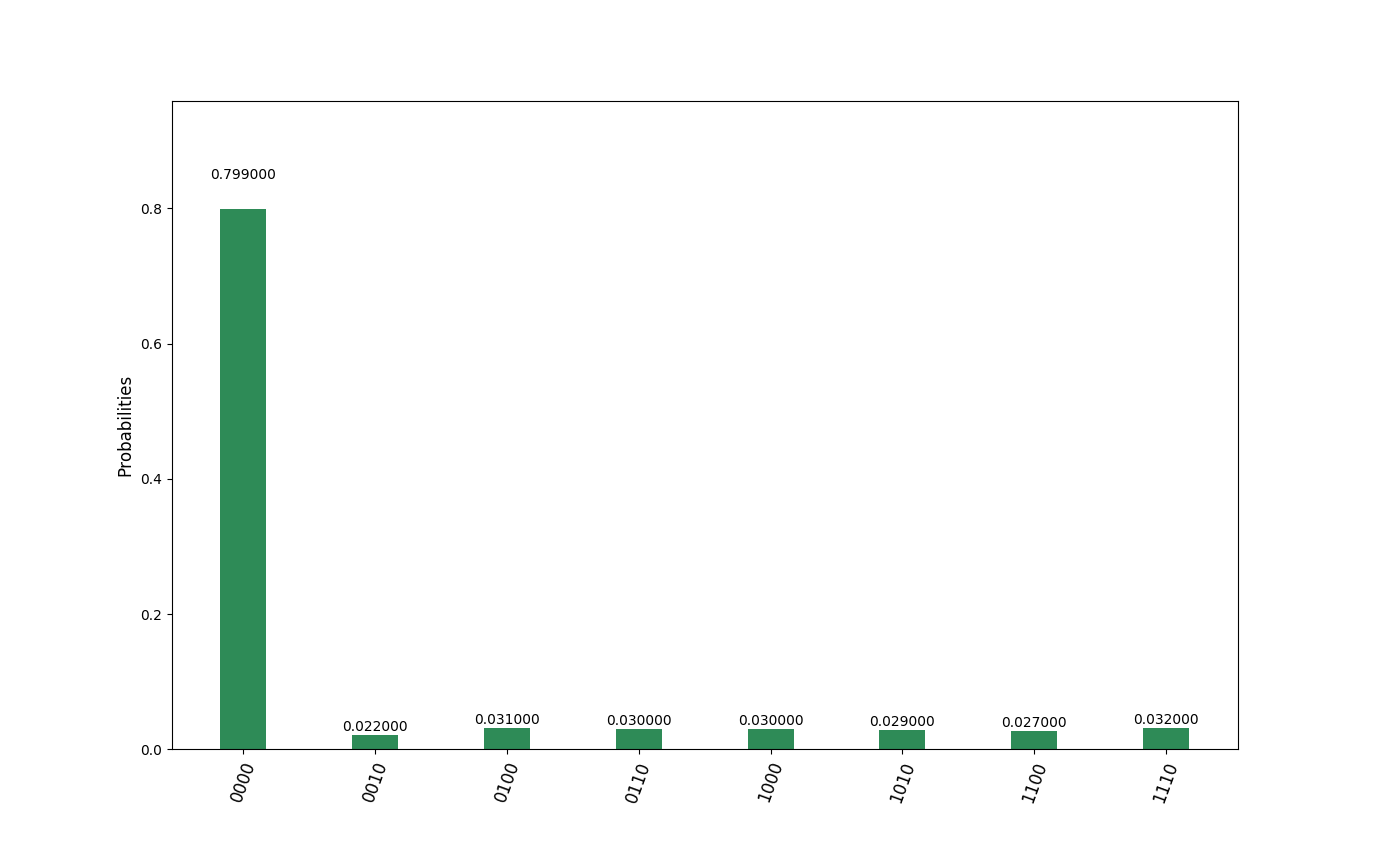
\includegraphics[scale=0.32]{Grover_results/Grover_n=3,m=1.png} & 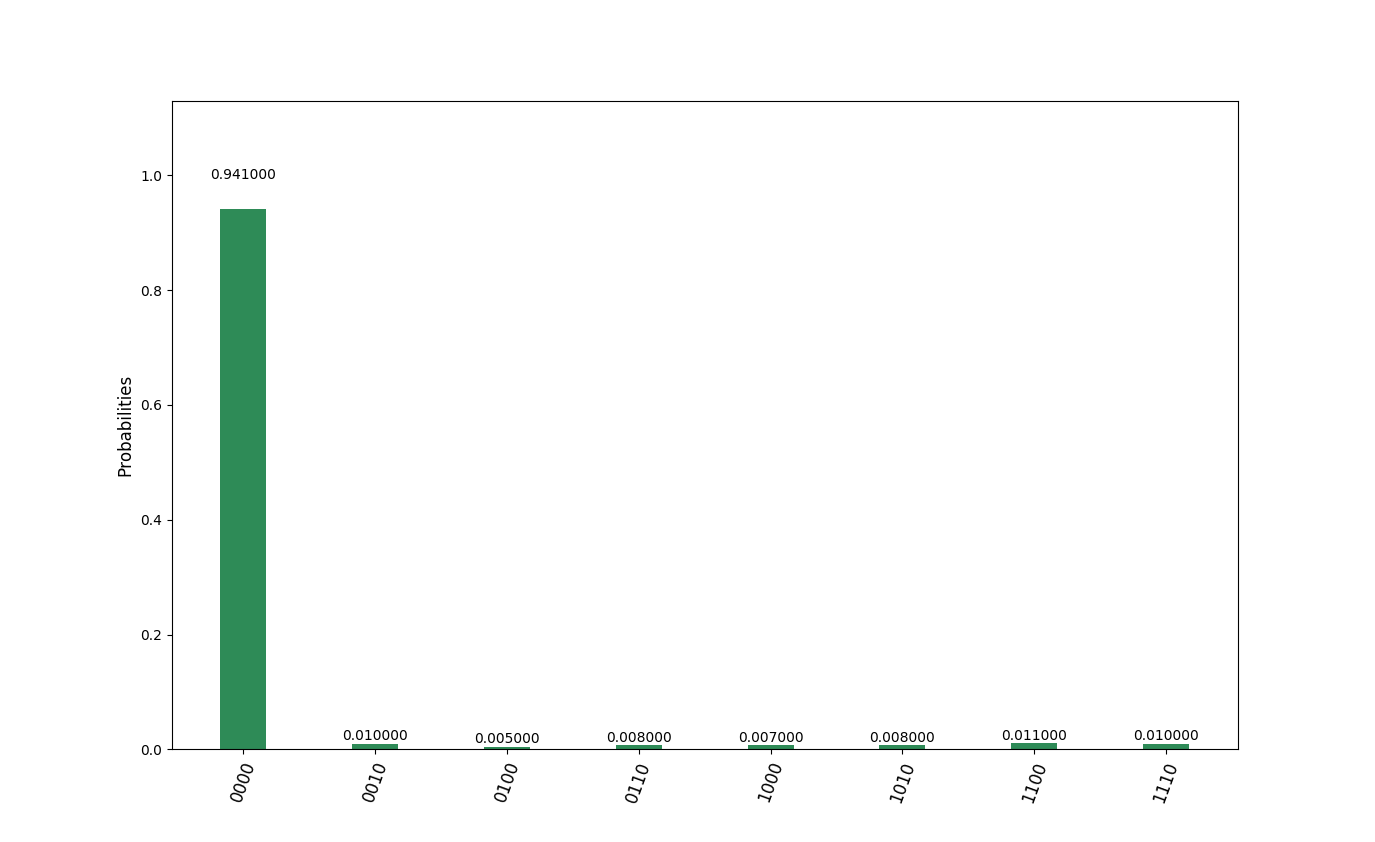
\includegraphics[scale=0.32]{Grover_results/Grover_n=3,m=2.png} \\ \hline
        n = 3, m = 3 & n = 3, m = 4 \\ \hline
        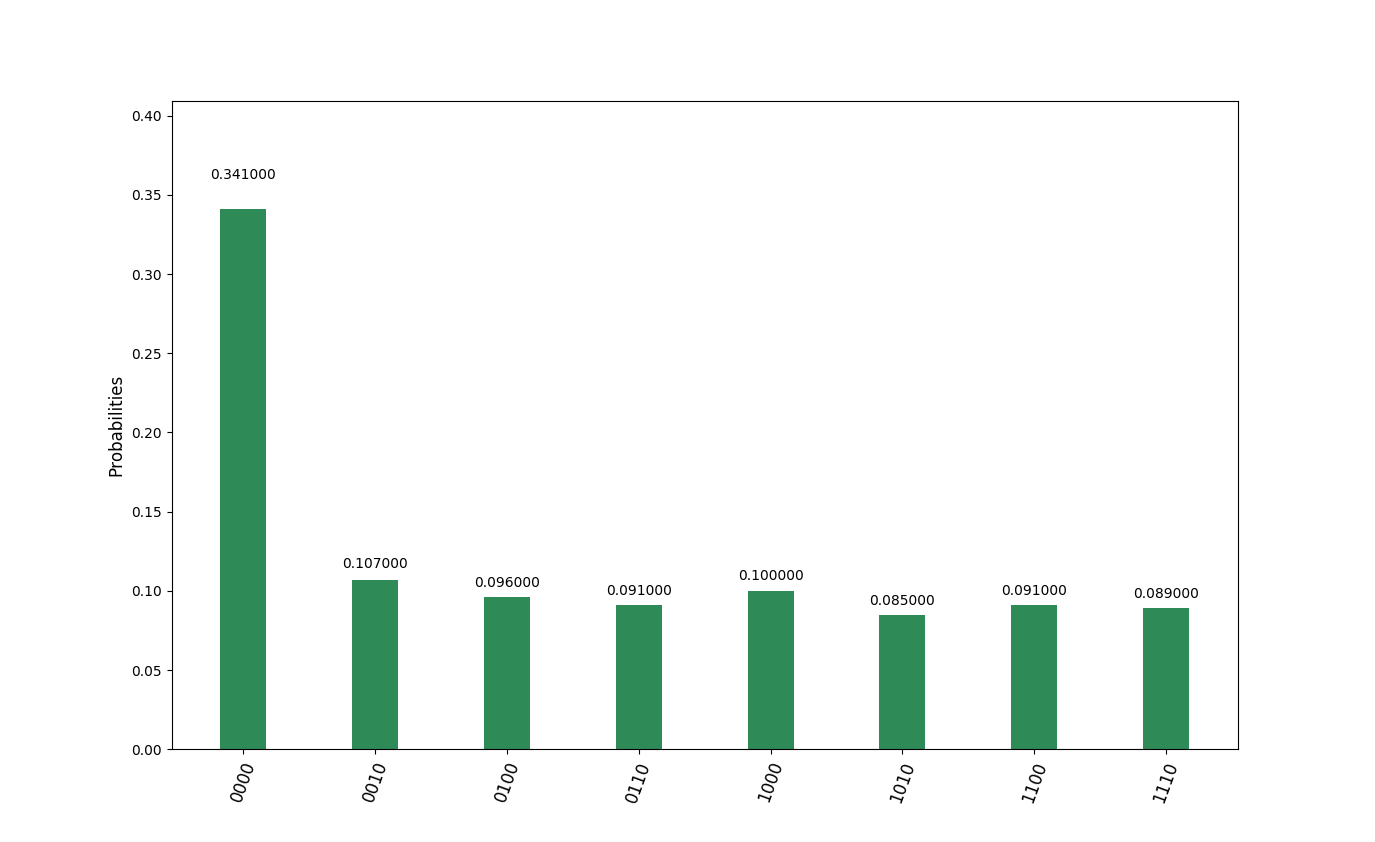
\includegraphics[scale=0.32]{Grover_results/Grover_n=3,m=3.png} & 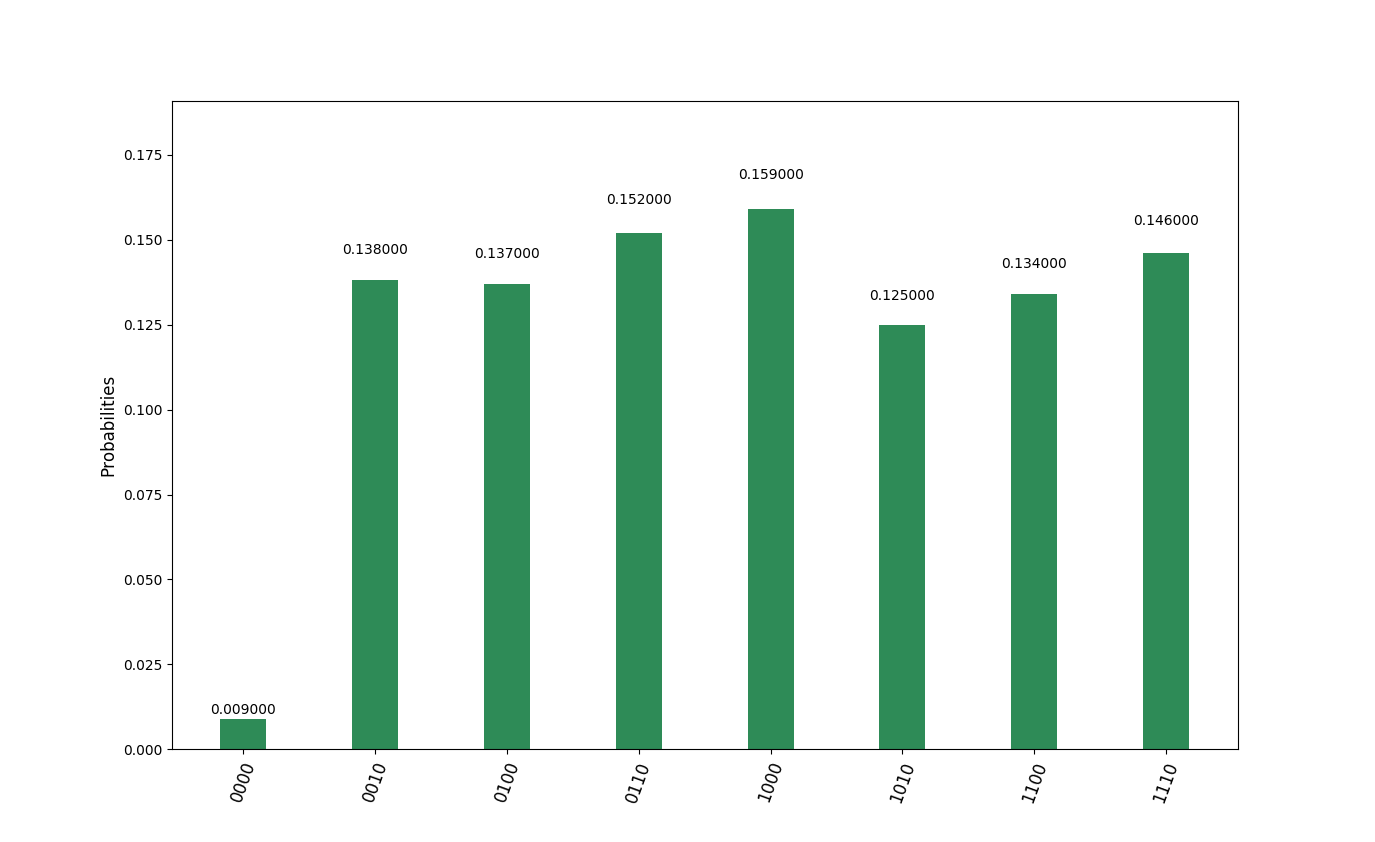
\includegraphics[scale=0.32]{Grover_results/Grover_n=3,m=4.png} \\ \hline
    \end{tabular}
\end{table}
\end{landscape}

\newpage
\begin{landscape}
\begin{table}[ht]
    \begin{tabular}{c c} 
        \hline
        n = 3, m = 5 & n = 3, m = 6 \\ \hline
        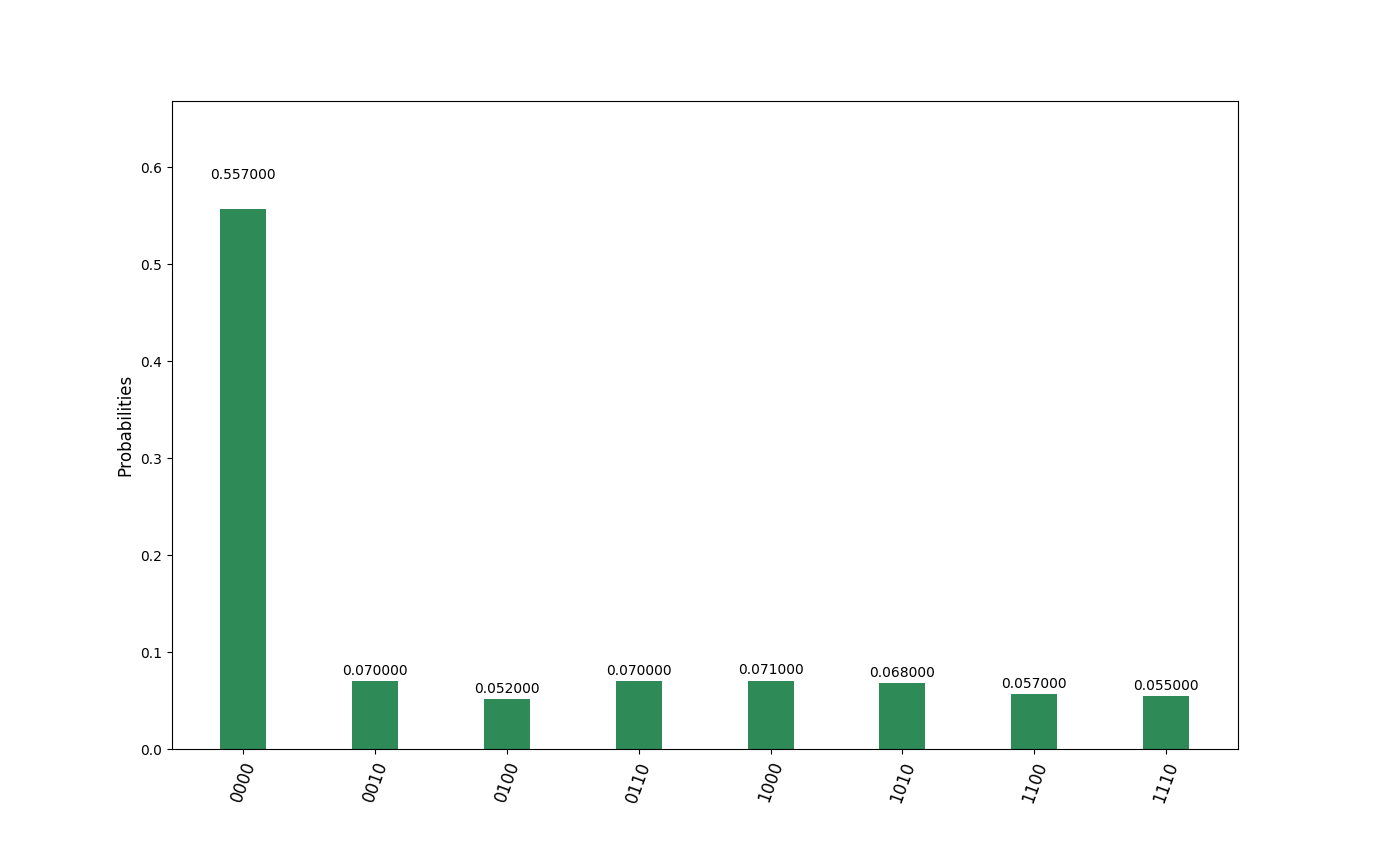
\includegraphics[scale=0.32]{Grover_results/Grover_n=3,m=5.png} & 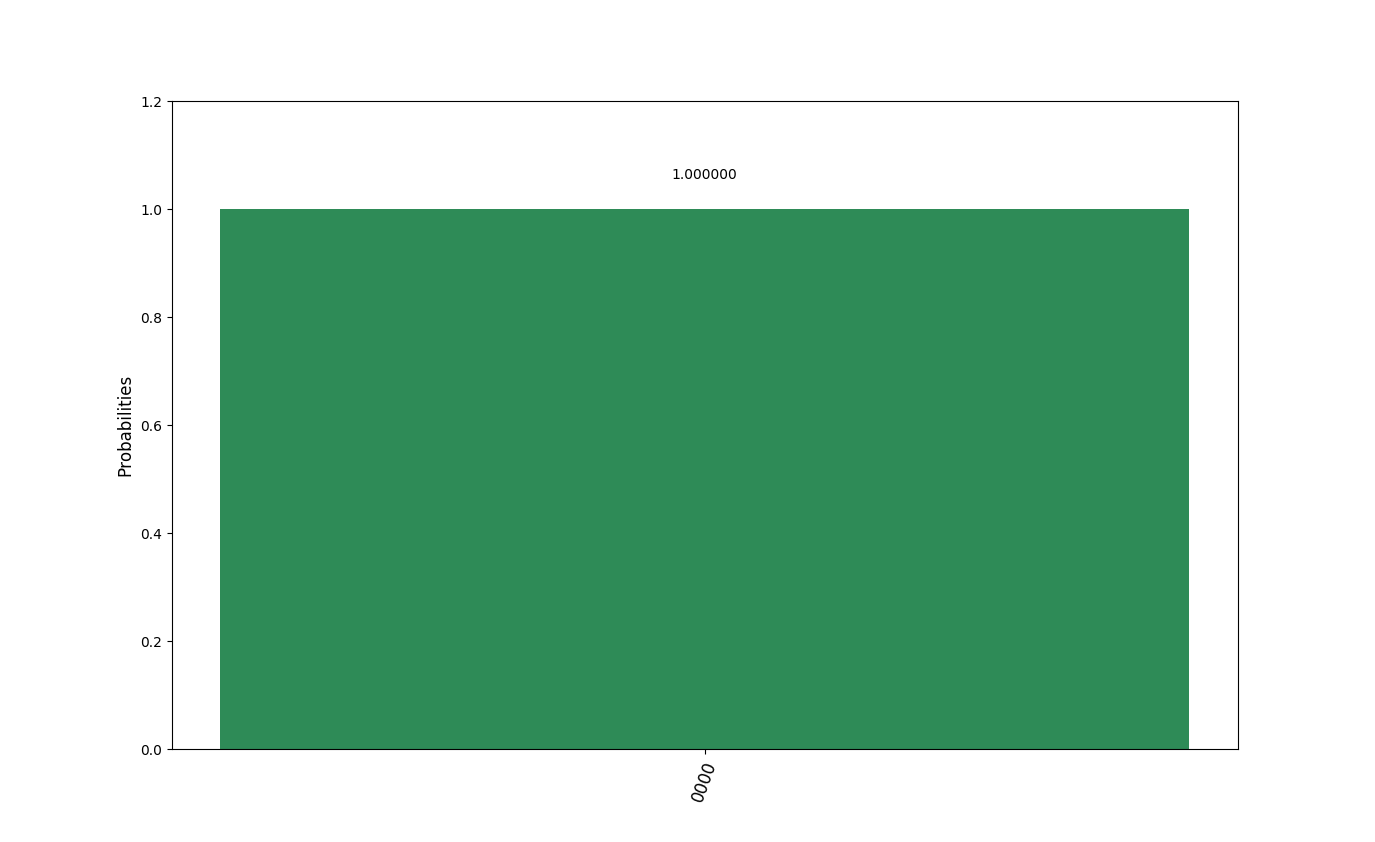
\includegraphics[scale=0.32]{Grover_results/Grover_n=3,m=6.png} \\ \hline
        n = 3, m = 7 & n = 3, m = 8 \\ \hline
        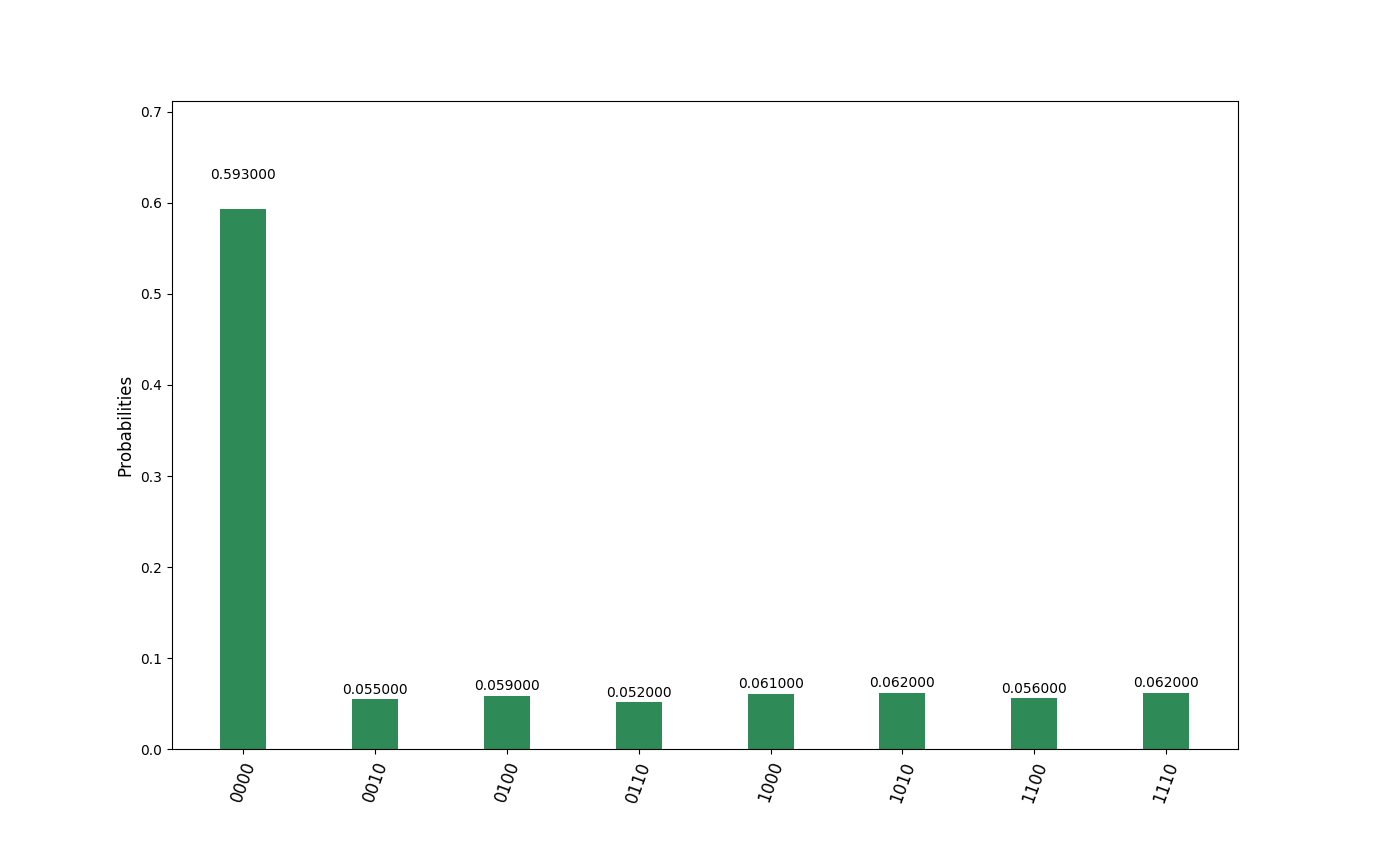
\includegraphics[scale=0.32]{Grover_results/Grover_n=3,m=7.png} & 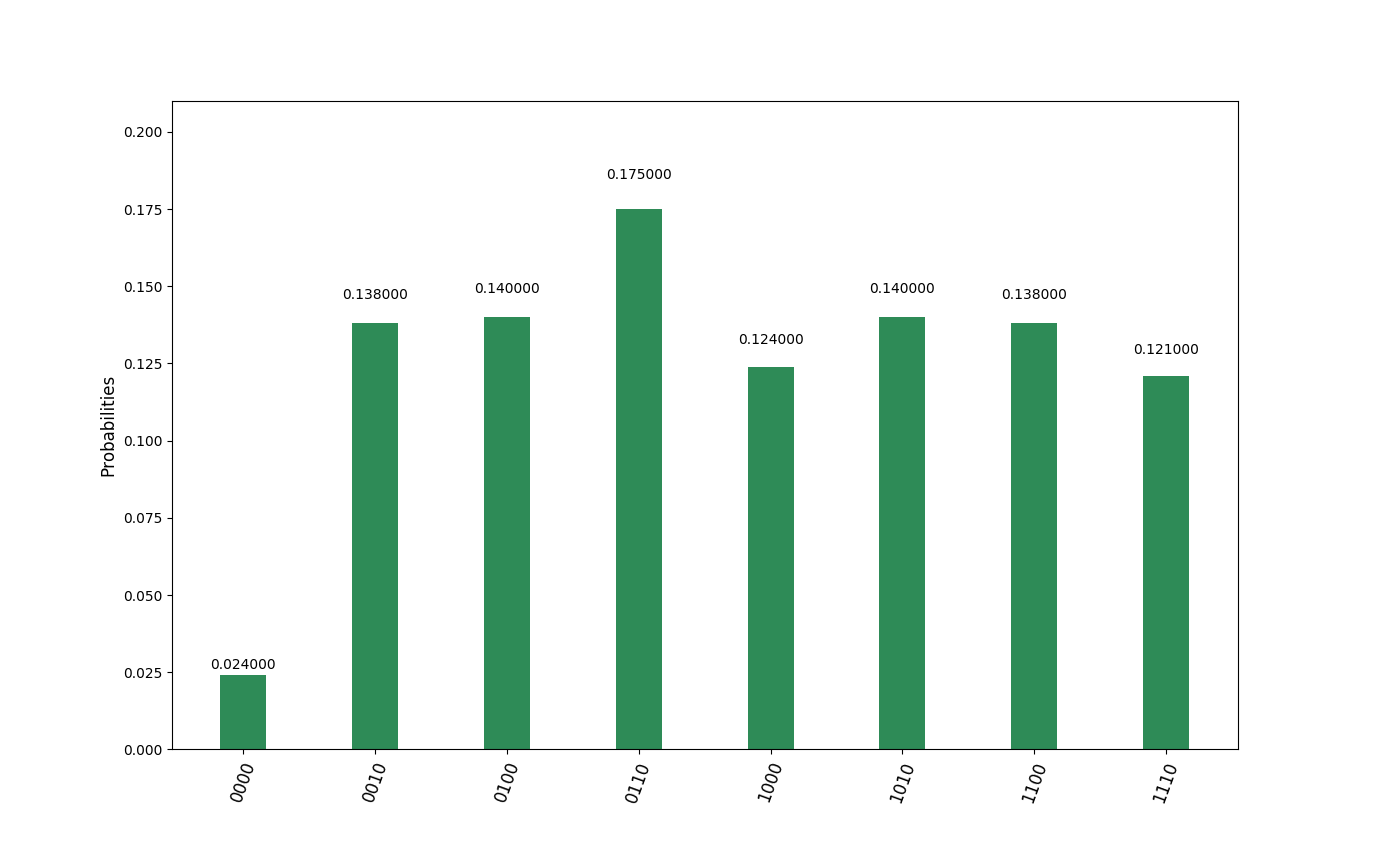
\includegraphics[scale=0.32]{Grover_results/Grover_n=3,m=8.png} \\ \hline
    \end{tabular}
\end{table}
\end{landscape}

\newpage
\begin{landscape}
\begin{table}[ht]
    \begin{tabular}{c c} 
        \hline
        n = 3, m = 9 & n = 3, m = 10 \\ \hline
        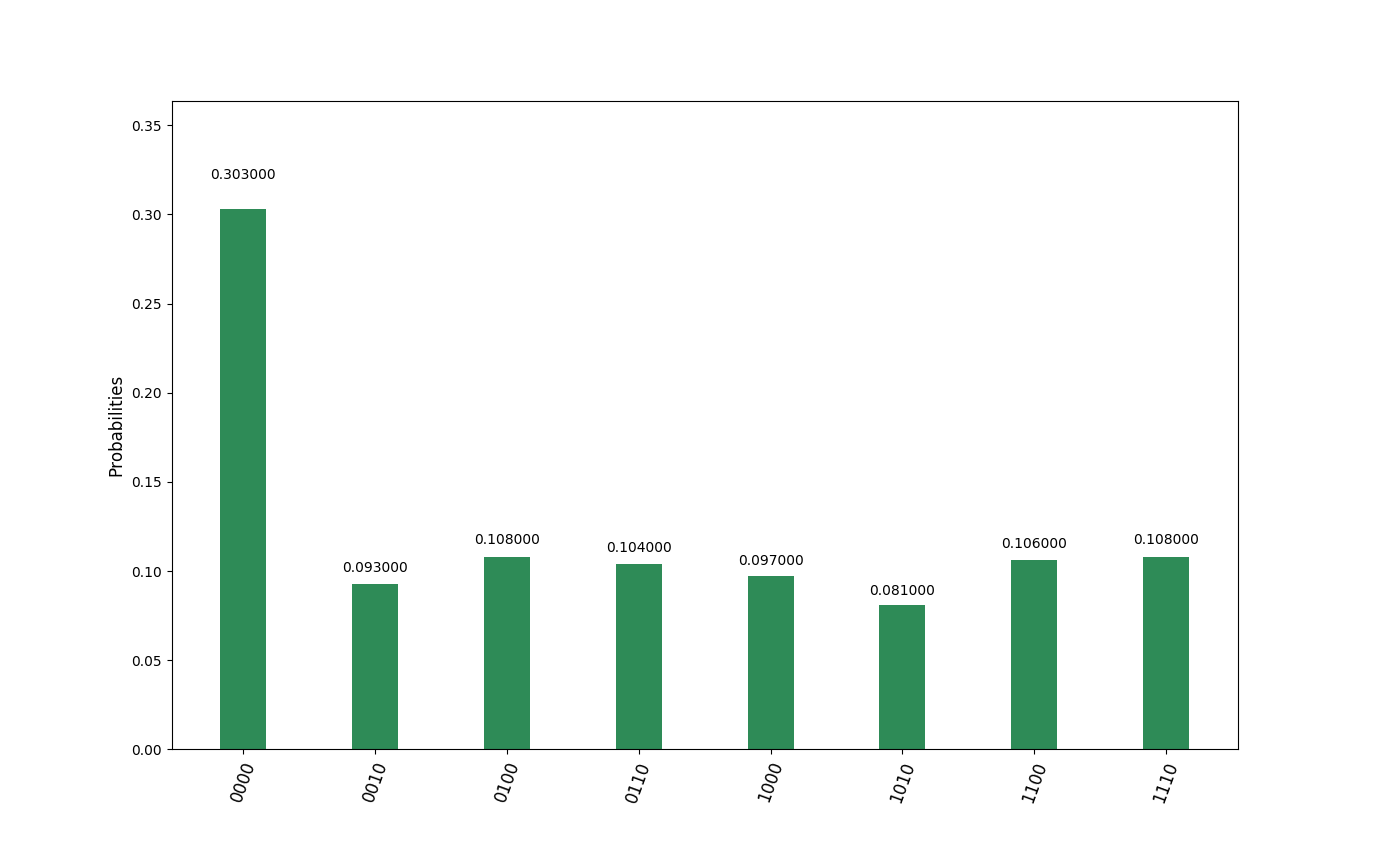
\includegraphics[scale=0.32]{Grover_results/Grover_n=3,m=9.png} & 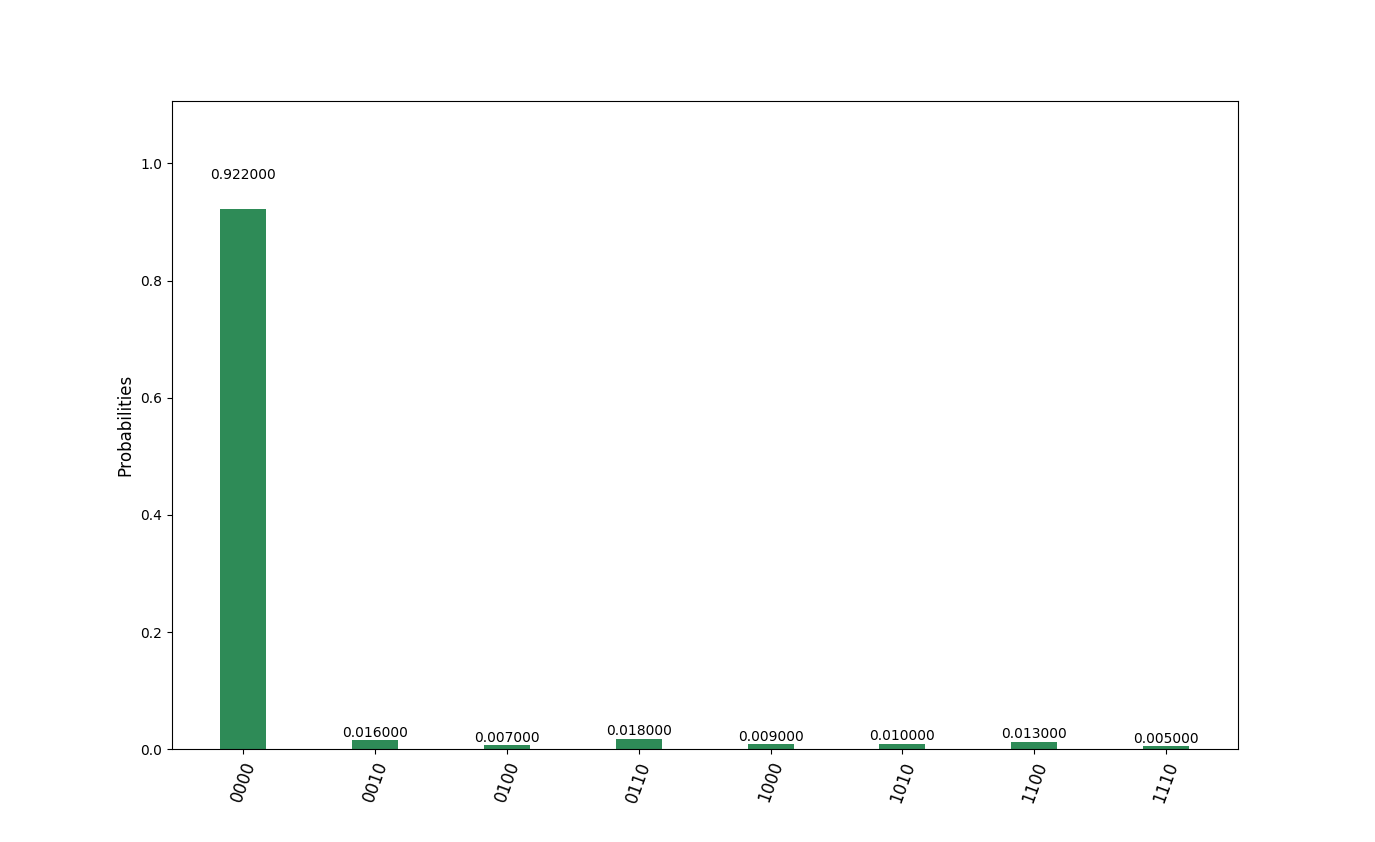
\includegraphics[scale=0.32]{Grover_results/Grover_n=3,m=10.png} \\ \hline
        n = 3, m = 11 & n = 3, m = 12 \\ \hline
        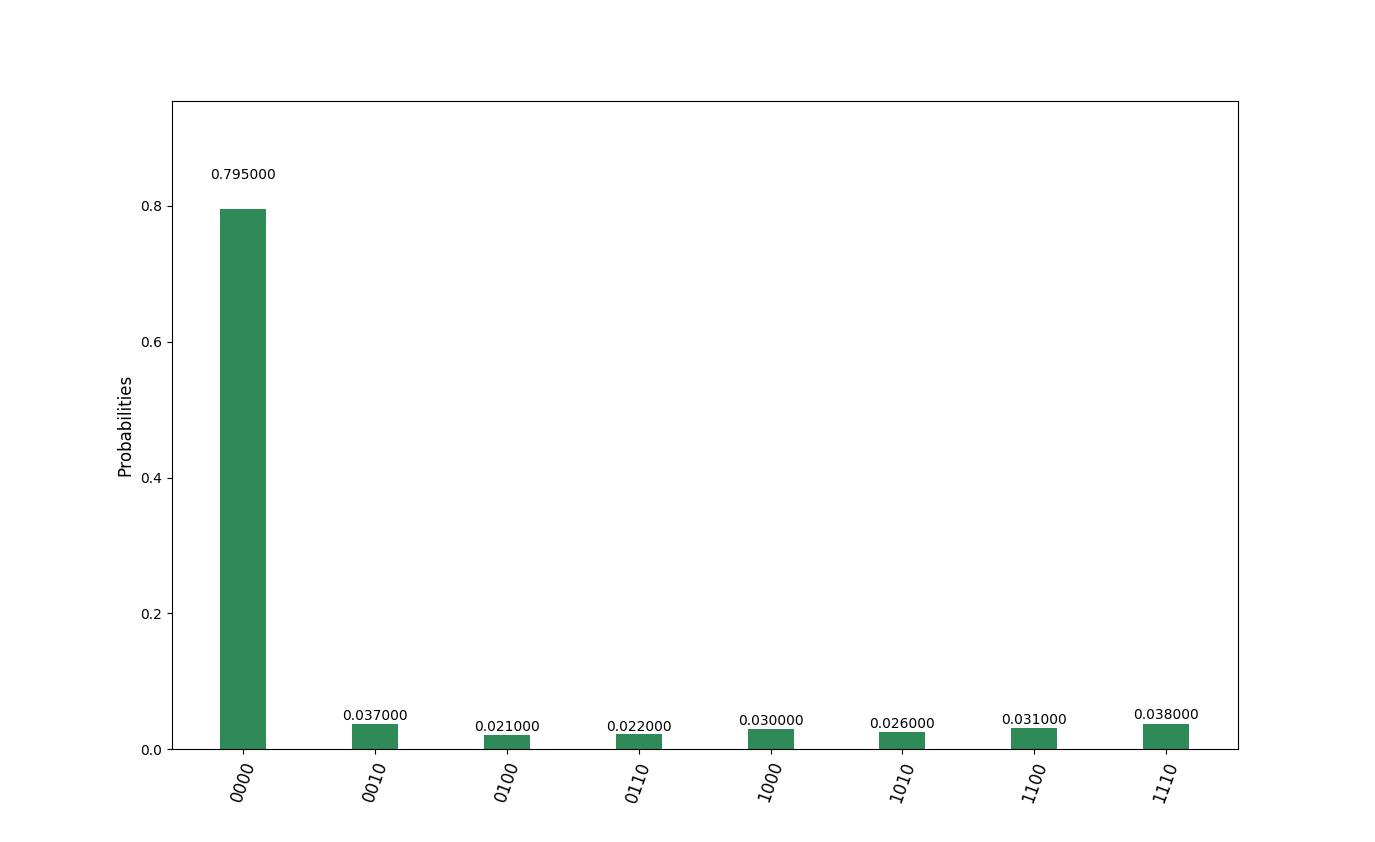
\includegraphics[scale=0.32]{Grover_results/Grover_n=3,m=11.png} & 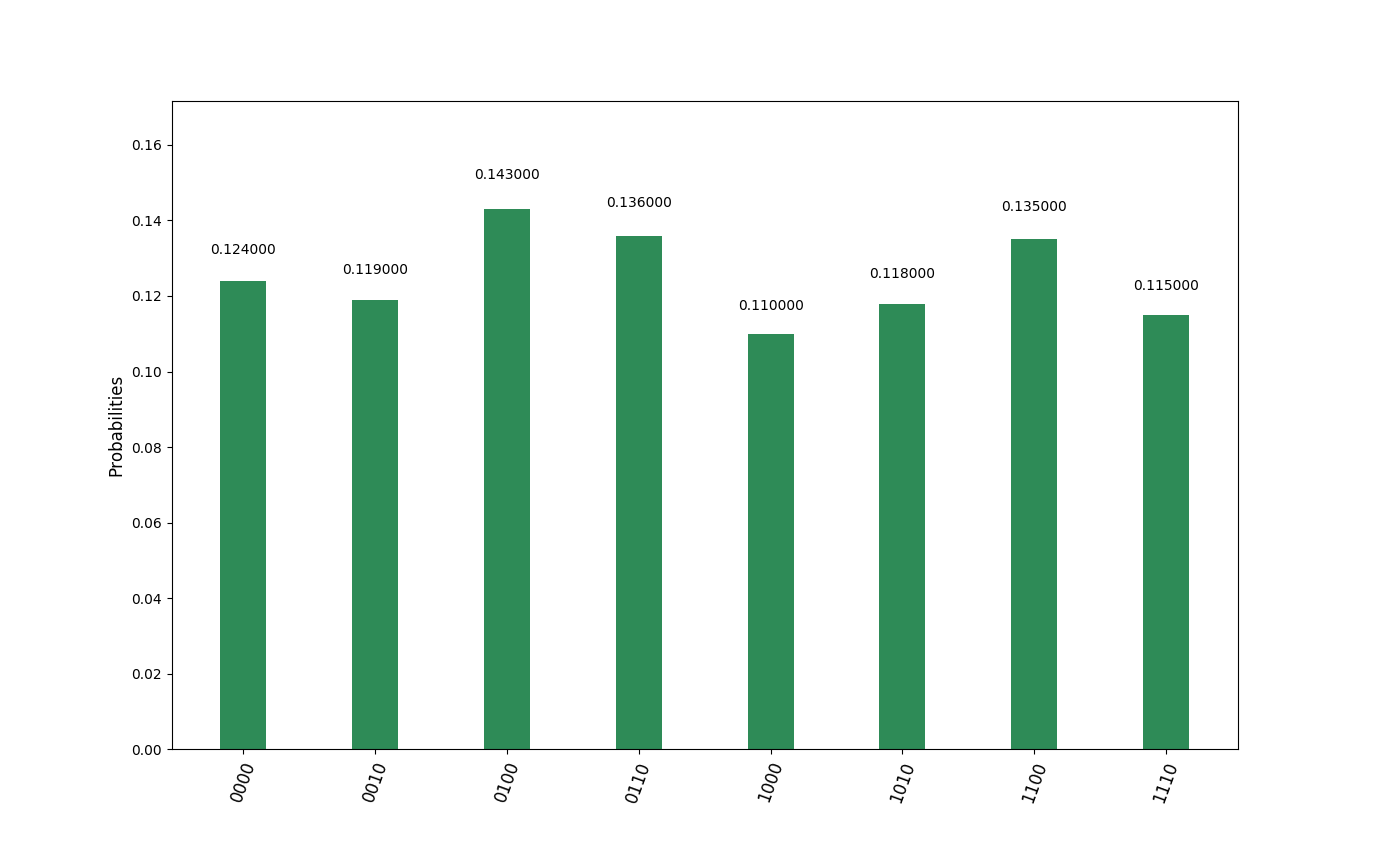
\includegraphics[scale=0.32]{Grover_results/Grover_n=3,m=12.png} \\ \hline
    \end{tabular}
\end{table}
\end{landscape}

\newpage
\begin{landscape}
\begin{table}[ht]
    \begin{tabular}{c c} 
        \hline
        n = 5, m = 1 & n = 5, m = 2 \\ \hline
        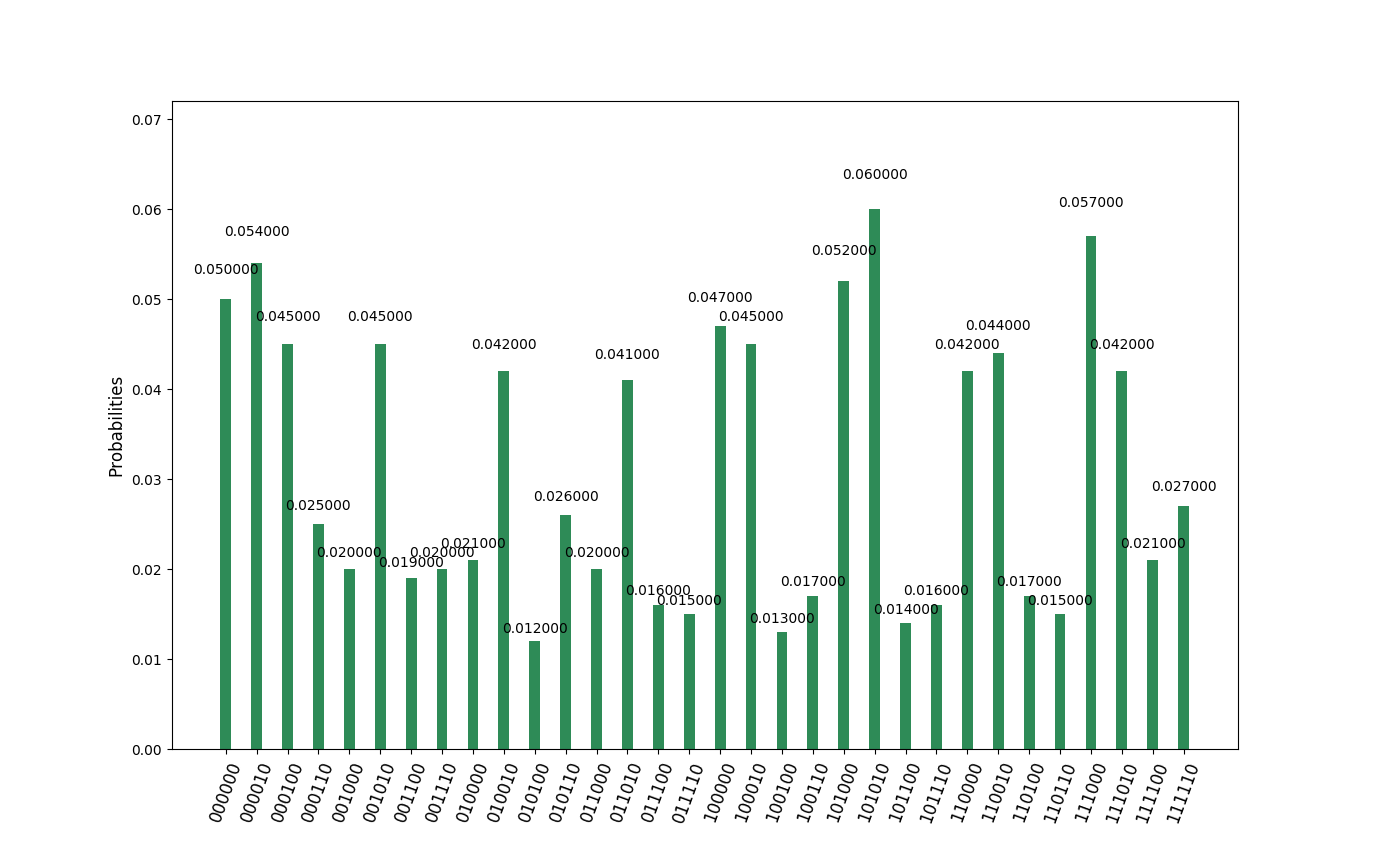
\includegraphics[scale=0.32]{Grover_results/Grover_n=5,m=1.png} & 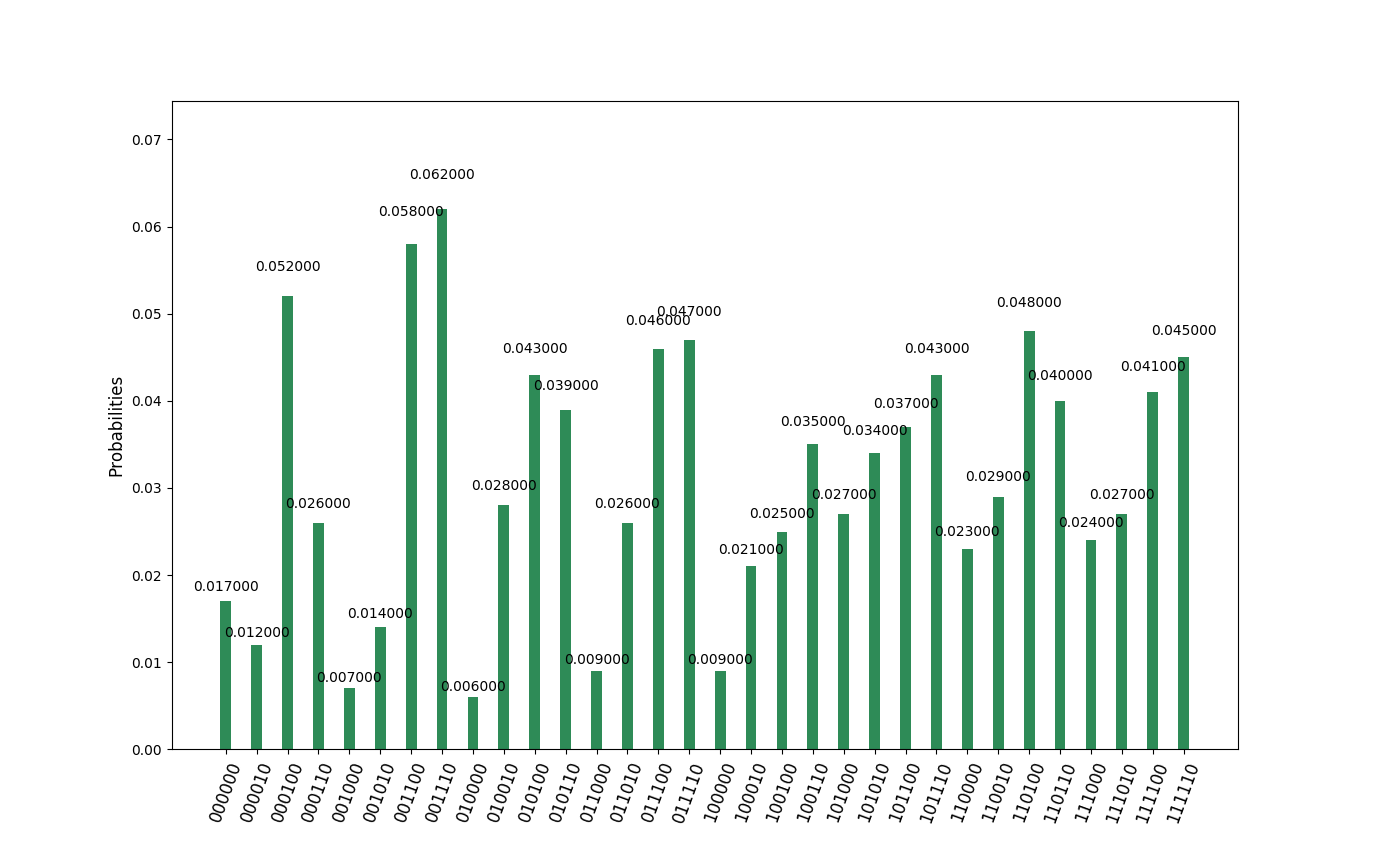
\includegraphics[scale=0.32]{Grover_results/Grover_n=5,m=2.png} \\ \hline
        n = 5, m = 3 & n = 5, m = 4 \\ \hline
        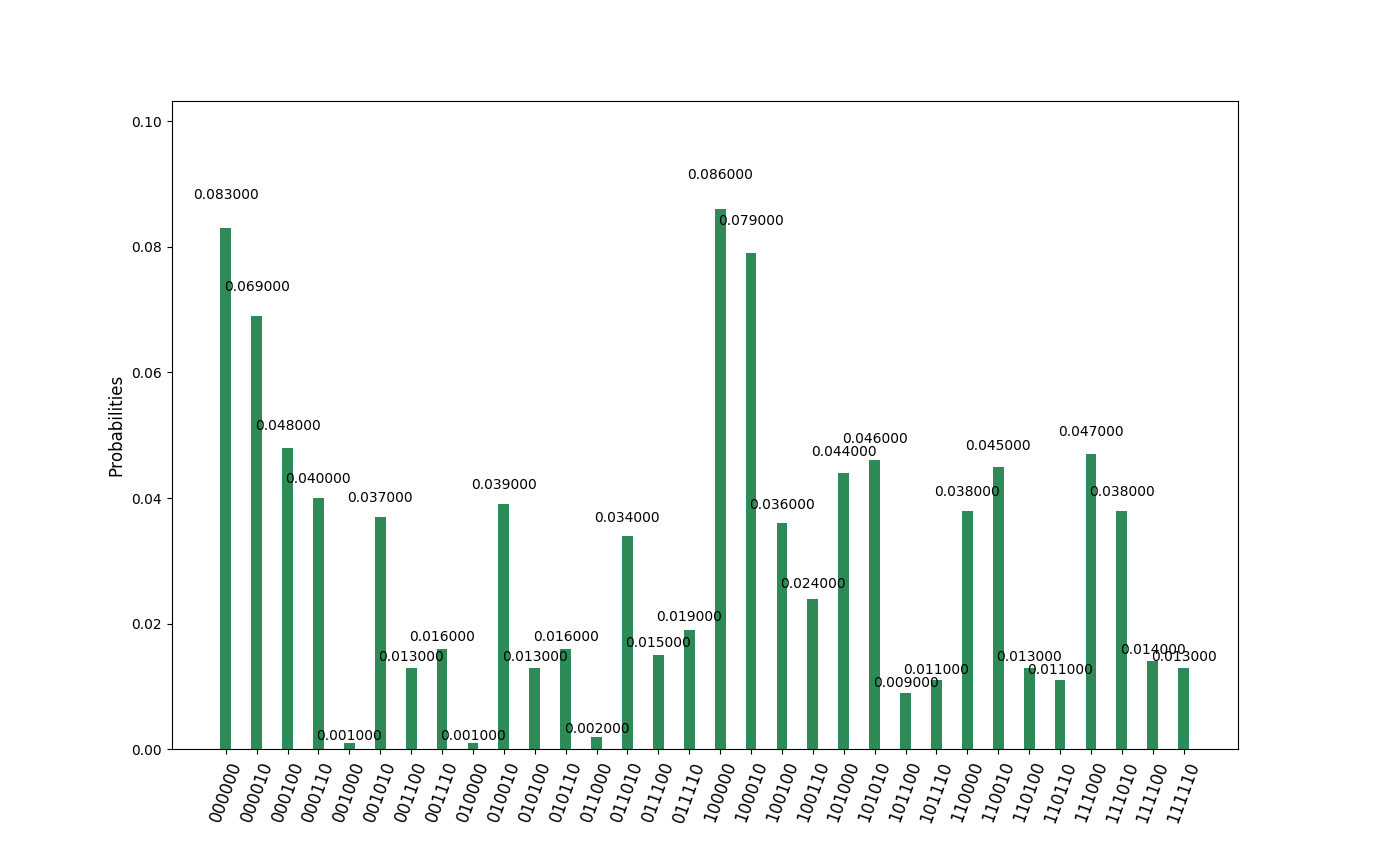
\includegraphics[scale=0.32]{Grover_results/Grover_n=5,m=3.png} & 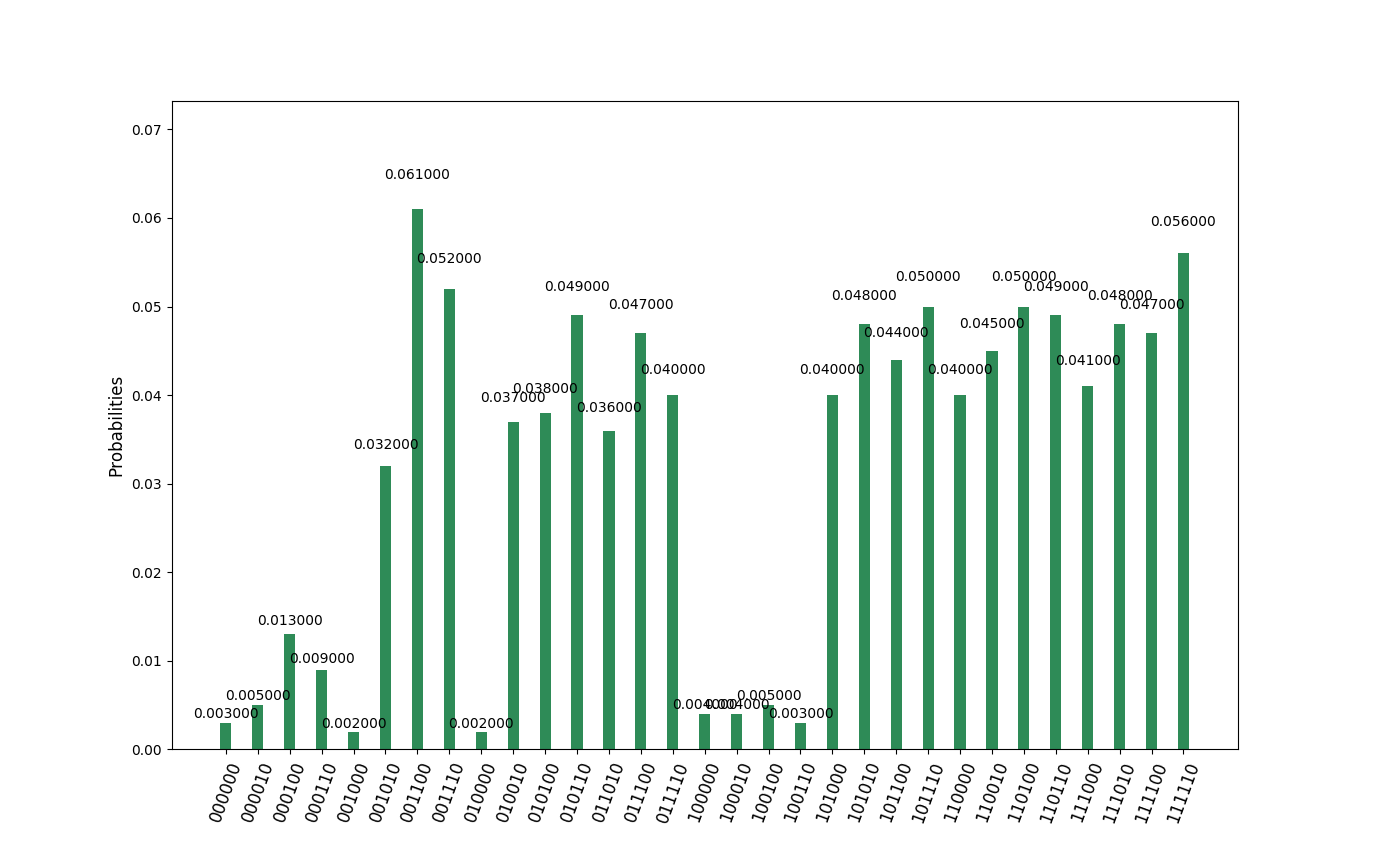
\includegraphics[scale=0.32]{Grover_results/Grover_n=5,m=4.png} \\ \hline
    \end{tabular}
\end{table}
\end{landscape}

\newpage
\begin{landscape}
\begin{table}[ht]
    \begin{tabular}{c c} 
        \hline
        n = 5, m = 5 & n = 5, m = 6 \\ \hline
        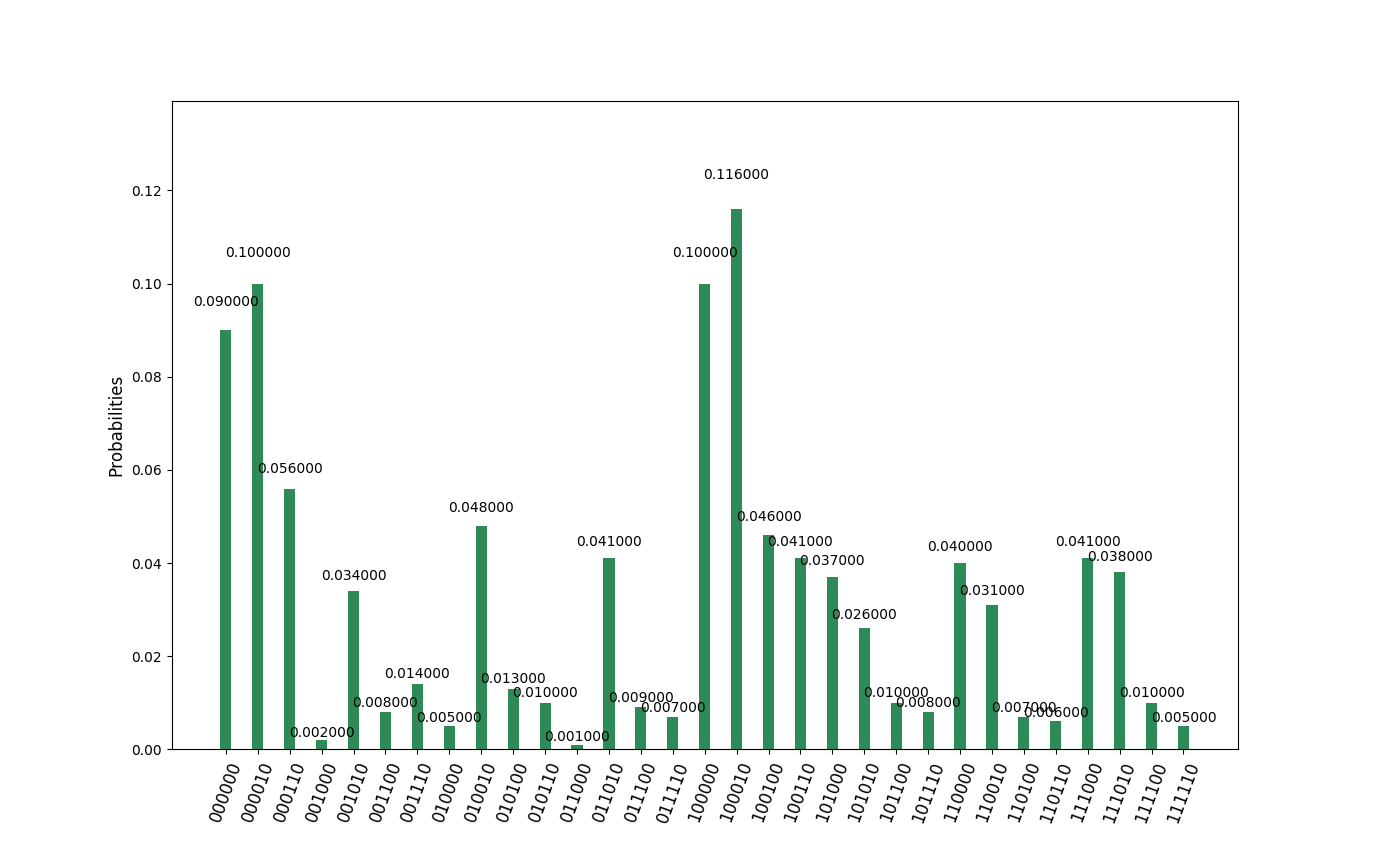
\includegraphics[scale=0.32]{Grover_results/Grover_n=5,m=5.png} & 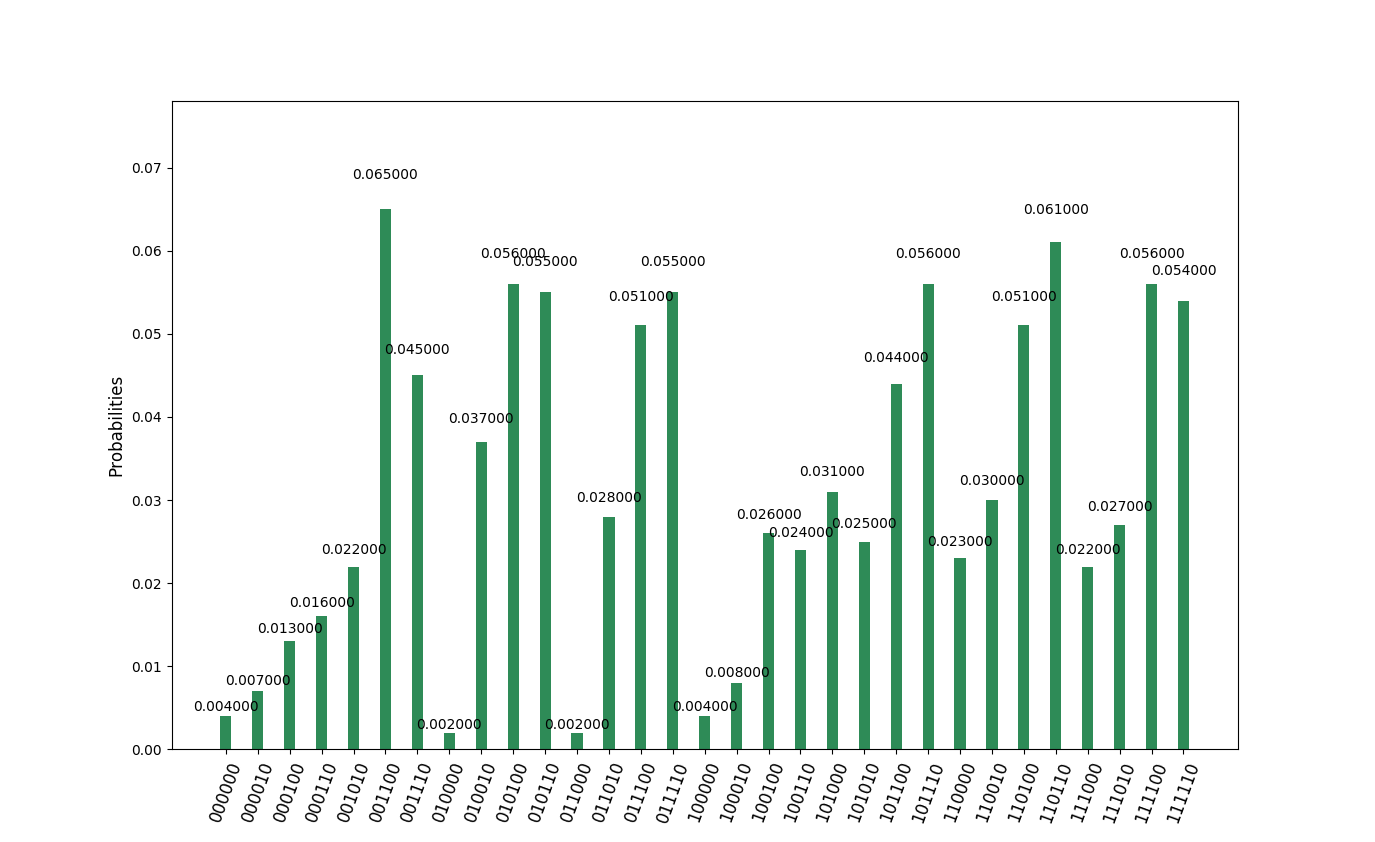
\includegraphics[scale=0.32]{Grover_results/Grover_n=5,m=6.png} \\ \hline
        n = 5, m = 7 & n = 5, m = 8 \\ \hline
        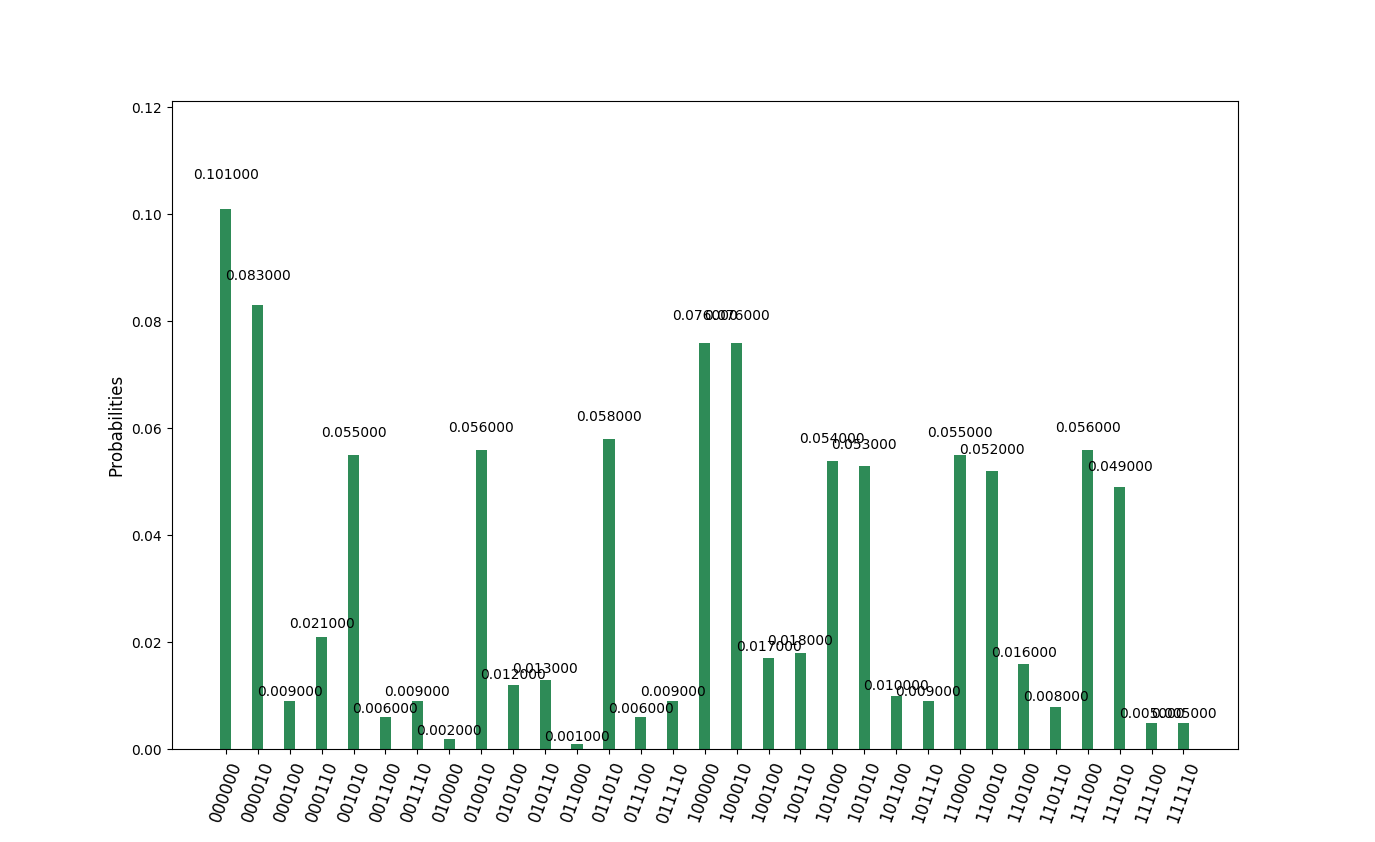
\includegraphics[scale=0.32]{Grover_results/Grover_n=5,m=7.png} & \includegraphics[scale=0.32]{Grover_results/Grover_n=5,m=8.png} \\ \hline
    \end{tabular}
\end{table}
\end{landscape}

\newpage
\begin{landscape}
\begin{table}[ht]
    \begin{tabular}{c c} 
        \hline
        n = 5, m = 9 & n = 5, m = 10 \\ \hline
        \includegraphics[scale=0.32]{Grover_results/Grover_n=5,m=9.png} & \includegraphics[scale=0.32]{Grover_results/Grover_n=5,m=10.png} \\ \hline
        n = 5, m = 11 & n = 5, m = 12 \\ \hline
        \includegraphics[scale=0.32]{Grover_results/Grover_n=5,m=11.png} & \includegraphics[scale=0.32]{Grover_results/Grover_n=5,m=12.png} \\ \hline
    \end{tabular}
\end{table}
\end{landscape}
	\cleardoublepage

\end{document}

